% Vorlage Version 1.0 vom 4.10.2021

% Doppelseitges Layout
\documentclass[a4paper, 12pt, twoside, openright]{report} 

% Einseitiges Layout
% \documentclass[a4paper, 12pt]{report} 

\raggedbottom
\usepackage{longtable}
\usepackage{lipsum}					    % Als Platzhalter für gewisse Stellen
\usepackage{ngerman}					% Deutsche Silbentrennung etc.
\usepackage[utf8]{inputenc}        	    % Umlaute in .tex Files normal schreibbar
                                        % Unter texnic-center alle Quelldateien unter Codierung ANSI abspeichern
                                        % Auf Unixsystemen ISO 8859-15
\usepackage{helvet}						% Helvetic als Schriftart
\usepackage{courier}					% Courier als Schriftart für Listings
\usepackage{fancyhdr}					% Kopf- und Fußzeilen ändern
\usepackage{a4}							% A4 Randeinstellungen
\usepackage{makeidx}					% Indexkommandos
\usepackage{listings}					% Für zeilennummerierte Listings mit Hintergrund
\usepackage{color}					    % Für grauen Hintergrund in Listings
\usepackage{setspace}					% Größerer Zeilenabstand
\usepackage{graphicx}					% Grafiken einbinden
\usepackage{sectsty}					% Format der Überschriften umändern
\usepackage{hyperref}
\usepackage{float}
\usepackage{pdfpages}					% Fremde pdfs einbinden
\usepackage[font={scriptsize}]{caption}
\usepackage{emptypage}
\usepackage{enumitem}
\usepackage[table]{xcolor}              % Tabellen farbig gestalten



% Dokumentationen zu den Paketen finden sich im Installationsordner 
% (normalerweise C:\Programme\texmf) unter docs und dort auch im Unterverzeichnis latex.

% Das Kompilieren des Dokuments benötigt bis zu 3 Durchläufe im alle Referenzen und
% Literatureinträge korrekt einzubinden.

%----------------------------------------------------------------------------------
% Listings 
%----------------------------------------------------------------------------------

%Definition des Aussehens der externen Listings
\def\source#1#2#3{     %  Sprache, Caption, Dateiname 
  %\global\advance\Sourcenummer by 1 
  %\index{Listing #1 #2}
  %\textbf{Listing-\the\Sourcenummer: #2}
  \lstinputlisting[language=#1,caption=#2]{#3} 
}

% Beispiele für eine Verwendung
%--------------------------------------------------------------------------------
% \source{xml}{\texttt{faces-config.xml}}{sources/faces-config.xml}
%
% \source{java}{\texttt{beans.UserBean.java}}{sources/jsf/user/UserBean.java}
%---------------------------------------------------------------------------------


% Definition des Aussehens der internen Listings
\definecolor{listinggray}{gray}{1.0}

%-------------------------------------------------------------------------
% Neues Listingformat
% --- kleine Schrift
% --- Keywords färbig
%-------------------------------------------------------------------------

\definecolor{dkgreen}{rgb}{0,0.6,0}
\definecolor{gray}{rgb}{0.5,0.5,0.5}
\definecolor{mauve}{rgb}{0.58,0,0.82}
\definecolor{orange}{RGB}{240, 105, 12}
\definecolor{green}{RGB}{156, 206, 43}

\lstset{ %
  language=Java,                  % the language of the code
  basicstyle=\footnotesize\ttfamily\bfseries,       % the size of the fonts that are used for the code
  numbers=left,                   % where to put the line-numbers
  numberstyle=\footnozesize,      % the size of the fonts that are used for the line-numbers
  stepnumber=1,                   % the step between two line-numbers. If it's 1, each line 
                                  % will be numbered
  numbersep=5pt,                  % how far the line-numbers are from the code
  backgroundcolor=\color{white},  % choose the background color. You must add \usepackage{color}
  showspaces=false,               % show spaces adding particular underscores
  showstringspaces=false,         % underline spaces within strings
  showtabs=false,                 % show tabs within strings adding particular underscores
  frame=single,                   % adds a frame around the code
  tabsize=2,                      % sets default tabsize to 2 spaces
  captionpos=b,                   % sets the caption-position to bottom
  breaklines=true,                % sets automatic line breaking
  breakatwhitespace=false,        % sets if automatic breaks should only happen at whitespace
  title=\lstname,                 % show the filename of files included with \lstinputlisting;
                                  % also try caption instead of title
  numberstyle=\tiny\color{gray},  % line number style
  keywordstyle=\color{blue},      % keyword style
  commentstyle=\color{dkgreen},   % comment style
  stringstyle=\color{mauve},      % string literal style
  escapeinside={\%*}{*)},         % if you want to add a comment within your code
  morekeywords={*,...}            % if you want to add more keywords to the set
}


% Eigene Kommandos
\newcommand{\zb}{z.B.\ }				              %z.B.
\newcommand{\tm}{\texttrademark \ }			          %TM - Zeichen
\newcommand{\sk}[1]{\emph{siehe Kapitel \ref{#1}}}	  %siehe Kapitel <Referenz>
\newcommand{\lil}[1]{\emph{Listing \ref{#1}}}		  %Listing <Referenz>
\newcommand{\slil}[1]{\emph{siehe Listing \ref{#1}}}  %siehe Listing <Referenz>
\newcommand{\pr}{$\rightarrow\ $}			          %Pfeil nach rechts


%-------------------------------------------------------------------------------
% Uebersichten i Anhang richtig formatieren
%-------------------------------------------------------------------------------

\makeatletter
\renewcommand*\l@section{\@dottedtocline{2}{3.8em}{4em}}
\renewcommand*\l@subsection{\@dottedtocline{2}{3.8em}{4em}}
\renewcommand*\l@subsubsection{\@dottedtocline{2}{3.8em}{4em}}
\renewcommand*\l@figure{\@dottedtocline{1}{2.8em}{3em}}
\renewcommand*\l@lstlisting{\@dottedtocline{1}{2.8em}{3em}}
\makeatother

% Es soll ein Index für diese Diplomarbeit erzeugt werden
%\makeindex

% Längen- und Absatzeinstellungen
\parindent=0pt		    % Kein Einrücken der ersten Zeile eines Absatzes
\parskip=12pt			% 12pt Abstand zwischen 2 Absätzen
\doublespacing 	        % Doppelter Zeilenabstand
\onehalfspacing	        % Eineinhalbfacher Zeilenabstand

\setlength{\headheight}{15pt}		% Kopfzeile vergrößern (wegen 12pt Schriftgröße)	
\addtolength{\textwidth}{1.5cm}	    % Rechten Rand verkleinern
\addtolength{\evensidemargin}{-1.5cm}


%--------------------------------------------------------------------------
% Beginn Dokument
%--------------------------------------------------------------------------


\begin{document}
	\sffamily						% Schriftart setzen
	\allsectionsfont{\sffamily}		% Schrift für Überschrift setzen
	
	\pagestyle{empty}
\singlespacing
\sffamily

\begin{flushleft}
	
\includegraphics[scale=0.40]{images/HTLstp-RGB.png} \\
% 	\vspace{-2cm}
% 	\hspace{7cm}
% 	\Huge
% 	\textbf{- Diplomarbeit -} \\
% 	\hrulefill
\end{flushleft}
\vspace{-2.5cm}
\begin{flushright}
	
\includegraphics[scale=0.10]{images/HTL.jpg} \\
% 	\vspace{-2cm}
% 	\hspace{7cm}
% 	\Huge
% 	\textbf{- Diplomarbeit -} \\
% 	\hrulefill
\end{flushright}

\vspace{-2.7cm}
\begin{center}
\textbf{HTBLuVA St. Pölten}\\
\textbf{Höhere Abteilung für Informatik}
\end{center}
\vspace{-0.7cm}
\hrulefill

\begin{center}
\vspace{2cm}
\huge
\textbf{DIPLOMARBEIT}

\huge
\textbf{Entwicklung eines mobilen, cloudbasierten Webfrontends für eine bestehende Arztsoftware}

\large
\textbf{im Projekt CGM MAXX LITE}
\end{center}

\begin{flushleft}
\large
\vspace{3cm}
\begin{small}
\begin{tabular}{lp{2cm}l}

\textbf{Ausgeführt im Schuljahr 2024/25 von:} &  & \textbf{Betreuer/Betreuerin:} \\
\\																
Emily Atzinger, 5BHIF-01 & & Dipl.-Ing. Werner Gitschthaler, BEd  \\
Matthias Zimmermann, 5BHIF-23 & & Ing. Mag. Andreas Schönbichler \\
Oskar Brödler, 5BHIF-02 \\
Hannes Koppensteiner, 5BHIF-12 \\
\end{tabular}
\end{small}
\end{flushleft}

\vspace{1cm}

St.Pölten, am \today			% Externe .tex Datei für Titel einbinden
	\cleardoublepage				% Neue Seite beginnen

	
%-----------------------------------------------------------------
% Vorwort
%-----------------------------------------------------------------
	
	\pagestyle{plain}							%Nur Fußzeile mit Seitennummer anzeigen lassen
	\pagenumbering{roman}					%Römische Nummerierung vor der eigentlichen Diplomarbeit
	\setcounter{page}{1}					%Bei 1 mit Nummerierung beginnen

    \addcontentsline{toc}{chapter}{Vorwort}
	\addcontentsline{toc}{section}{Erklärung}	%Erklärung händisch ins Inhaltsverzeichnis einfügen
	\begin{flushleft}
\Large
\textbf{Eidesstattliche Erklärung\\}
\vspace{1.5cm}
\end{flushleft}


Ich erkläre an Eides statt, dass ich die vorliegende Diplomarbeit selbständig und ohne fremde Hilfe verfasst, andere als die angegebenen Quellen
und Hilfsmittel nicht benutzt und die den benutzten Quellen wörtlich und inhaltlich entnommenen Stellen als solche erkenntlich gemacht habe.

\begin{center}
    \vspace{1.5cm}
	\rule{200pt}{1pt} \\
	Emily Atzinger

    \vspace{1.5cm}
    \rule{200pt}{1pt} \\
    Matthias Zimmermann
	
	\vspace{1.5cm}
	\rule{200pt}{1pt} \\
	Oskar Brödler

    \vspace{1.5cm}
    \rule{200pt}{1pt} \\
    Hannes Koppensteiner
\end{center}

\vspace{1.5cm}

St.Pölten, am \today
				%Externe .tex Datei für Erklärung einfügen
	\cleardoublepage									%Neue Seite beginnen
	\phantomsection
	
	
	\addcontentsline{toc}{section}{Danksagungen}
	\begin{flushleft}
    \Large
    \textbf{Danksagungen\\}
    \vspace{1.5cm}
	\large
    \cleardoublepage
    
\end{flushleft}
	\cleardoublepage
	\phantomsection
	

	\addcontentsline{toc}{section}{Zusammenfassung}
	\begin{flushleft}
	
	\subsection*{Zusammenfassung}

	\subsubsection*{Entwicklung eines mobilen, cloudbasierten Webfrontends für eine bestehende Arztsoftware im Projekt CGM MAXX LITE:}

    Das Ziel dieser Diplomarbeit ist die Entwicklung eines mobilen Prototyps der bestehenden Arztsoftware CGM MAXX, der auf Smartphones und Tablets genutzt werden kann, um Arbeitsabläufe in Arztpraxen zu optimieren.

    Zu Beginn wird die Softwarearchitektur beleuchtet, indem Herausforderungen und deren Bedeutung hervorgehoben werden. Anschließend folgt eine Anforderungsanalyse als Grundlage für die Wahl eines Architekturstils. Dabei wird eine Auswahl relevanter cloudbasierter Architekturen beschrieben.
    Zudem werden DevOps-Praktiken und Infrastructure as Code (IaC) betrachtet, um eine effiziente Bereitstellung und Wartung von Software in der Cloud zu ermöglichen.

    Das zweite Kapitel befasst sich mit der Gestaltung einer benutzerfreundlichen Weboberfläche. Dabei werden die wesentlichen Prinzipien der User Experience (UX) vorgestellt und Methoden erläutert, wie diese in der Praxis getestet und umgesetzt werden können. Im Anschluss wird der Prozess von der Konzeptentwicklung bis zur fertigen App beschrieben, einschließlich der praktischen Umsetzung und der verwendeten Designansätze.

    Das dritte Kapitel widmet sich der Qualität des Quellcodes und behandelt Methoden zur Sicherstellung der Verständlichkeit des Codes, um eine einfache Weiterentwicklung in der Zukunft zu gewährleisten. Zudem wird auf die Bedeutung von statischer Codeanalyse und Code Reviews eingegangen, um Fehler frühzeitig zu identifizieren und die Wartbarkeit des Codes zu verbessern.
    Ein weiteres Thema ist Refactoring, das dazu dient, den Code zu optimieren, ihn strukturiert und skalierbar zu gestalten, sodass eine
    langfristige Erweiterung des Projekts möglich ist.

   Im letzten Teil der Diplomarbeit wird erklärt, wie die Qualität des Codes anhand von Testing sichergestellt werden kann. Dabei liegt der Fokus auf Behavior-Driven Development (BDD) und End-to-End (E2E)-Testing. Mithilfe von Selenium und Cucumber wird die gesamte Benutzererfahrung getestet, indem Szenarien beschrieben werden, die das Verhalten des Systems aus der Sicht des Benutzers simulieren. Dies ermöglicht eine enge Zusammenarbeit zwischen Entwicklern und Fachabteilungen. Zusätzlich wird das Backend-Testing behandelt, wobei Stubs zum Einsatz kommen, um Komponenten zu simulieren und die Funktionalität des Systems zu überprüfen.

\end{flushleft}
	\cleardoublepage
	\phantomsection
	
	\addcontentsline{toc}{section}{Abstract}
	\begin{flushleft}
	
	\subsection*{Abstract}

	\subsubsection*{Development of a Mobile, Cloud-Based Web Frontend for an Existing Medical Software in the CGM MAXX LITE Project:}

    The goal of this thesis is to develop a mobile prototype of the existing medical software CGM MAXX, which can be used on smartphones and tablets to optimize workflows in medical practices.

    The thesis begins by exploring the software architecture, highlighting the challenges and their significance. This is followed by a requirements analysis that serves as the basis for selecting an architectural style. A selection of relevant cloud-based architectures is described. Additionally, DevOps practices and Infrastructure as Code (IaC) are considered to enable efficient deployment and maintenance of software in the cloud.
    
    The second chapter focuses on the design of a user-friendly web interface. It introduces the fundamental principles of User Experience (UX) and explains methods to test and implement these principles in practice. The process from concept development to the final app is then described, including the practical implementation and design approaches used.
    
    The third chapter is dedicated to the quality of the source code and discusses methods for ensuring the understandability of the code to facilitate future development. The importance of static code analysis and code reviews is also highlighted to identify errors early and improve the maintainability of the code. Another topic is refactoring, which aims to optimize the code, making it structured and scalable, so that the project can be easily expanded in the long term.
    
    The final part of the thesis explains how the quality of the code can be ensured through testing. The focus here is on Behavior-Driven Development (BDD) and End-to-End (E2E) testing. Using Selenium and Cucumber, the entire user experience is tested by describing scenarios that simulate the system's behavior from the user's perspective. This enables close collaboration between developers and business departments. Additionally, backend testing is addressed, using stubs to simulate components and verify the functionality of the system.

\end{flushleft}
	\cleardoublepage
	\phantomsection
	
	\normalsize

	\markright{INHALTSVERZEICHNIS}
	\addcontentsline{toc}{chapter}{Inhaltsverzeichnis}
	\tableofcontents
	\cleardoublepage
	\phantomsection
	
		
%-----------------------------------------------------------------
% Kopfzeilen definieren
%-----------------------------------------------------------------
	\pagestyle{fancyplain}

	\renewcommand{\sectionmark}[1]{\markright{\thesection\ #1}}
	\renewcommand{\chaptermark}[1]{\markright{\thechapter\ #1}}
	\lhead[\fancyplain{}{\sffamily\sl\thepage}]{\fancyplain{}{\sffamily\sl\rightmark}}
	\rhead[\fancyplain{}{\sffamily\sl\rightmark}]{\fancyplain{}{\sffamily\sl\thepage}}
	\cfoot{}

	\pagenumbering{arabic}	%Seiten wieder normal nummerieren
	\setcounter{page}{1}		%Bei 1 beginnen

%--------------------------------------------------------------------------
% Kapitel einfügen
%--------------------------------------------------------------------------

\clearpage
%\input{textparts/MZ/...}
\clearpage
\chapter{Softwarearchitektur mit Schwerpunkt auf cloudbasierten Systemen}

    \section{Allgemeines} \label{Allgemeines}
    % --- E I N L E I T U N G ---

\subsection{Einleitung}

Softwarearchitektur - ein Begriff, den nahezu jede/r Softwareentwickler/in kennt.
Viele sind sich ihrer Bedeutung bewusst, doch nur die wenigsten schenken ihr die nötige Beachtung.
In einer Zeit, in der sich die Technik stetig weiterentwickelt und die Konkurrenz täglich wächst, ist es entscheidend, immer einen Schritt voraus zu sein, um erfolgreich zu bleiben.

Aus diesem Grund versuchen Entwickler/innen, so viele neue Funktionalitäten wie möglich zu implementieren, ohne sich ausgiebig mit der darunterliegenden Architektur zu befassen.
Anfangs scheint diese Vorgehensweise gut zu funktionieren, bis der Punkt erreicht wird, an dem es so gut wie unmöglich ist, die Software weiterzuentwickeln oder zu verändern. Dies führt oft zu schwerwiegenden Problemen wie erhöhtem Wartungsaufwand, schwer nachvollziehbaren Abhängigkeiten und letztlich hohen Kosten.
Um solche Szenarien vorzubeugen, ist es wichtig, sich genauer mit der Architektur der zu entwickelnden Software zu beschäftigen und sich darüber bewusst zu werden, wie umfangreich dieses Themengebiet überhaupt ist.
Hierbei geht es nicht nur um die Strukturierung des Codes, sondern auch darum, wie die einzelnen Komponenten eines Systems miteinander interagieren. Durch eine gut durchdachte Architektur soll der gesamte Lebenszyklus des Softwaresystems unterstützt und so einfach wie möglich gestaltet werden. 
\cite[S. 10, S. 136-137]{EA:Book01}


% --- D E F I N I T I O N   V O N   S O F T W A R E A R C H I T E K T U R --- 

\subsection{Definition von Softwarearchitektur}

Um die Wichtigkeit der Softwarearchitektur zu begreifen, muss zunächst die Frage geklärt werden, was darunter zu verstehen ist. Dies ist jedoch gar nicht so einfach, da keine allgemein gültige, allumfassende Beschreibung existiert.

Grundsätzlich ist die Softwarearchitektur als etwas Dynamisches zu betrachten. Das bedeutet, dass sie sich durch die fortschreitende Entwicklung in der IT ständig verändert. Damit ist auch jede heute gültige Definition in wenigen Jahren wahrscheinlich wieder veraltet. \cite[S. 1-3]{EA:Book02}

Befasst man sich genauer mit dem Begriff \glqq Architektur\grqq, wird schnell deutlich, dass es auch hier zahlreiche unterschiedliche Definitionen gibt. Dazu zählen Folgende:

\begin{itemize}
    \item Organisation von Modulen, Verbindungen, Abhängigkeiten und Schnittstellen
    \item Modell, um das System als Ganzes zu verstehen
    \item Standards, Richtlinien und Einschränkungen
    \item Ergebnis strategischer und technischer Entscheidungen
\end{itemize}

Zusammenfassend kann gesagt werden, dass es sich hierbei um die \textbf{Struktur} eines bestimmten Objekts handelt. In diesem Fall um die Struktur eines Softwaresystems. \cite{EA:Web01}

Bass, Clements und Kazman beschreiben die Softwarearchitektur folgendermaßen:

\begin{quote}
    ``The software architecture of a program or computing system is the structure or structures of the system, which comprise software elements, the externally visible properties of those elements, and the relations among them.`` \cite[S. 3]{EA:Book03}
\end{quote}

Allerdings umfasst die Architektur weit mehr als nur die Struktur eines Systems. 
Im Mittelpunkt steht der Prozess der Architekturerstellung, bei dem architektonische Treiber wie funktionale und nicht-funktionale Anforderungen, Qualitätsmerkmale, Einschränkungen und Prinzipien in eine technische Lösung überführt werden. Dabei entsteht eine \textbf{Vision\footnote{Beschreibt einen wünschenswerten Zustand in der Zukunft}}, die an die Stakeholder kommuniziert werden muss, um eine einheitliche Sichtweise auf das zu entwickelnde Produkt zu gewährleisten. Nur so kann eine erfolgreiche Lösung geschaffen werden.
\cite{EA:Web01}

\clearpage

Um die zuvor definierten Aspekte der Softwarearchitektur weiter zu vertiefen, ist es hilfreich, das Thema in Teilbereiche zu zerlegen, die leichter beschrieben werden können.


% --- A P P L I K A T I O N S A R C H I T E K T U R ---

    \subsubsection{Applikationsarchitektur}

    Wenn man von der Architektur einer einzelnen, bereitstellbaren Applikation spricht, können sich die meisten Softwareentwickler/innen vermutlich etwas darunter vorstellen. Ein gutes Beispiel dafür ist eine Angular-Applikation.

    Im Wesentlichen geht es dabei um die \textbf{Organisation und Strukturierung des Codes}. 
    Dazu ist es notwendig zu verstehen, wie eine solche Applikation entworfen und implementiert wird. 
    Um dies zu erreichen, ist es essenziell, sich mit den spezifischen Elementen der eingesetzten Technologien sowie mit verschiedenen Entwurfsmustern, Frameworks und Bibliotheken auseinanderzusetzen.
    \cite{EA:Web01}


% --- S Y S T E M A R C H I T E K T U R ---

    \subsubsection{Systemarchitektur} \label{Softwarearchitektur}

    Die Systemarchitektur ist eine Stufe über der Applikationsarchitektur. Heutzutage besteht nämlich so gut wie jedes Softwaresystem aus mehreren auslieferbaren Einheiten, die miteinander interagieren. 
    Betrachtet man beispielsweise eine Arztsoftware, so hat diese eine Benutzeroberfläche, die von medizinischem Fachpersonal oder entsprechenden Hilfskräften bedient werden kann. Hinzu kommt ein im Hintergrund laufendes Backend, das auf die Aktionen von Anwender/innen reagiert und Daten aus einer oder mehreren Datenbanken abruft oder dort speichert.

    Diese separaten Applikationen müssen miteinander verbunden werden. Dabei ist zu beachten, dass diese auf unterschiedlichen Technologien basieren können, was unter Umständen zu Problemen führt. Das System wird also auf einer \textbf{höheren Ebene} betrachtet. 
    Der Fokus liegt auf der Integration einzelner Anwendungen in ein übergeordnetes System.

    Während sich die Applikationsarchitektur hauptsächlich mit Details, wie der genauen Implementierung einer bestimmten Funktionalität befasst, beschäftigt sich die Systemarchitektur sowohl mit \textbf{Software als auch Hardware}.
    Auch wenn die Hardware durch Virtualisierung und Cloud heute kein allzu großes Problem mehr darstellt, muss die Software irgendwo bereitgestellt werden.
    \cite{EA:Web01}


% --- S O F T W A R E A R C H I T E K T U R ---

    \subsubsection{Softwarearchitektur}

    Nachdem die Teilbereiche nun genauer beschrieben wurden, kann die Softwarearchitektur als \textbf{Kombination aus Applikations- und Systemarchitektur} charakterisiert werden.

    Die Softwarearchitektur umfasst sowohl die Struktur des Codes als auch das Zusammenspiel der einzelnen Komponenten im System.
    Dabei stehen Aspekte wie saubere Code-Struktur, Erweiterbarkeit und die Sicherstellung der Funktionalität des Systems im Vordergrund, insbesondere in Bezug auf Sicherheitsanforderungen, Leistungsoptimierungen und zukünftige Entwicklungen.
    \cite{EA:Web01}

    Robert C. Martin veranschaulicht das Konzept der Softwarearchitektur mit einem guten Beispiel. Plant ein/e Architekt/in ein Gebäude, so werden grundlegende Dinge, wie der Grundriss, die äußere Erscheinung und die Raumteilung, geplant. Allerdings gibt es auch einige Kleinigkeiten, die berücksichtigt werden müssen. Dazu zählt unter anderem die Planung von Lichtschaltern, Steckdosen, Heizkörpern und Leitungen.
    \cite[S. 4]{EA:Book01}

    Diese Details bezeichnet man als \textbf{\glqq Low-Level Details\grqq}, während die übergeordnete Ebene, die zuvor als Systemarchitektur definiert wurde, den \textbf{\glqq High-Level Details\grqq}\ entspricht. Beide Ebenen müssen beachtet werden, um ein Softwaresystem zuverlässig, sicher und wartbar zu gestalten.


% --- A U F G A B E N   U N D   Z I E L E ---

\subsection{Aufgaben und Ziele} \label{Aufgaben und Ziele}

Da nun klar sein sollte, was Softwarearchitektur ist und womit sie sich befasst, kann näher auf die Aufgaben und Ziele eingegangen werden. 
Prinzipiell ist es möglich, Software zu entwickeln, ohne sich intensiv mit dem Thema Architektur auseinanderzusetzen.
Ein gut durchdachtes Konzept kann jedoch viel Arbeit und die damit verbundenen Kosten sparen.

Ziel ist es, das Entwicklerteam sowie die Projektbeteiligten schlank zu halten, um die Kosten zu minimieren und die Wünsche des Auftraggebenden effizient zu erfüllen. Kurzgefasst lässt sich sagen, dass der \textbf{Aufwand minimiert} und die \textbf{Produktivität maximiert} werden soll. 
\cite[S. 4-5]{EA:Book01}

Weiters dient die Softwarearchitektur dazu, die \textbf{Qualität der Software sicherzustellen}, indem funktionale als auch nicht-funktionale Anforderungen berücksichtigt werden. Diese bilden die Grundlage für die Architektur der zu entwickelnden Software.
Was unter diesen Anforderungen zu verstehen ist, wird im Unterkapitel \ref{Anforderungsanalyse} näher beschrieben.
Die Architektur bietet nicht nur den Kund/innen einen Mehrwert, sondern auch das Entwicklerteam profitiert davon.
Sie kann als \textbf{Kommunikationswerkzeug} eingesetzt werden, um die Planung verschiedener Phasen einfacher zu gestalten und den Entwicklungsprozess zu beschleunigen. Außerdem kann die Architektur dabei helfen, das System besser zu analysieren, wodurch Änderungen schneller vorgenommen und Fehler leichter identifiziert werden können.
\cite{EA:Web02}

Eine gut überlegte Softwarearchitektur soll sowohl den Kund/innen als auch dem Projektteam zugutekommen: 
Aus Sicht der Kundschaft bedeutet das niedrige Kosten, aus Sicht des Projektteams einen reibungslosen Entwicklungsprozess mit klarer Kommunikationsgrundlage und ohne Einschränkungen für die Entwickler/innen.


% --- D I E   R O L L E   V O N   S O F T W A R E A R C H I T E K T / I N N E N ---

\subsection{Die Rolle von Softwarearchitekt/innen} \label{Die Rolle von Softwarearchitekt/innen}

Obwohl Entwickler/innen dafür verantwortlich sind, die Architektur der Software im Auge zu behalten und sich an dieser zu orientieren, ist es sinnvoll, eine Person zu haben, die sich auf dieses Themengebiet spezialisiert hat und stets den Überblick behält. Dies unterstützt nicht nur die Entwickler/innen dabei, den roten Faden nicht zu verlieren, sondern trägt auch dazu bei, die \textbf{Qualität der Software zu wahren}.

    \subsubsection{Definition}

    Genauso wie bei der Definition der Softwarearchitektur, ist es schwierig, die Rolle der Softwarearchitekt/innen eindeutig zu definieren. Grundsätzlich ist davon auszugehen, dass ein/e Softwarearchitekt/in eine erfahrene Fachkraft ist, welche die \textbf{Richtung vorgibt} und \textbf{für maximale Produktivität sorgt}. \\
    \cite[S. 136-137]{EA:Book01} \cite[S. 7-8]{EA:Book02}

    \subsubsection{Verantwortlichkeiten}

    Da die Erwartungen und Aufgaben von Softwarearchitekt/innen stark vom Projekt \\ abhängen, können hier nur ein paar allgemeine Grundsätze angeführt werden. \\ Diese sollten von jeder Person in dieser Rolle erfüllt werden.

    Wie bereits erwähnt, muss der/die Architekt/in in der Lage sein, das Projektteam, eine Abteilung oder sogar das gesamte Unternehmen in eine bestimmte Richtung zu lenken, indem er/sie bestimmte \textbf{Entscheidungen trifft}. Hierbei ist es entscheidend, sich nicht nur auf die persönliche Sichtweise zu beschränken, sondern auch dem Entwicklerteam die Möglichkeit zu geben, selbst Entscheidungen zu treffen. Ein Beispiel dafür wäre die Auswahl eines bestimmten Frameworks. Zudem muss der/die Architekt/in regelmäßig kontrollieren, ob diese Entscheidungen auch eingehalten werden. 

    Dass Softwarearchitekt/innen \textbf{viel Wissen und Erfahrung} benötigen, wurde bereits erwähnt. Allerdings reicht dies alleine nicht aus. 
    Um auf zukünftige Entwicklungen gefasst zu sein oder um mit der Konkurrenz mithalten zu können, ist es wichtig, sich laufend mit den neuesten Trends und Technologien auseinanderzusetzen.

    Es ist nicht nur technisches Können gefragt, sondern auch die \textbf{Fähigkeit, andere zu führen}. Dazu gehört die Koordination des Teams als auch die Kommunikation von Zielen, Prioritäten, Aufgaben und Deadlines.
    \cite[S. 7-8]{EA:Book02} \cite{EA:Web03}


% --- H E R A U S F O R D E R U N G E N   U N D   P R O B L E M E ---

\subsection{Herausforderungen und Probleme} \label{Herausforderungen und Probleme}

Wie im Abschnitt \ref{Aufgaben und Ziele} beschrieben, bietet eine gute Softwarearchitektur viele Vorteile. Es gibt jedoch einige Herausforderungen, die bewältigt werden müssen, um ihren vollen Nutzen ausschöpfen können. 
Werden diese Schwierigkeiten nicht überwunden, kann dies sowohl für die Kund/innen als auch für das durchführende Unternehmen zu ernsthaften Problemen führen. Im Folgenden werden die wesentlichen Herausforderungen beschrieben, deren Bewältigung entscheidend ist, um die später dargestellten Probleme zu vermeiden.

Eine der größten Schwierigkeiten besteht darin, \textbf{so viele Optionen wie möglich offen} zu \textbf{halten}.
Der Hintergedanke dabei ist, dass Software entwickelt wurde, um das Verhalten von Maschinen schnell verändern zu können, weswegen Flexibilität eine große Rolle spielt. Ein System muss nicht nur zuverlässig funktionieren, sondern auch leicht veränderbar sein.
Die Herausforderung besteht darin, die Business-Logik unabhängig von bestimmten technischen Details oder eingesetzten Technologien zu gestalten.

Ebenso ist es entscheidend, bereits \textbf{zu Beginn des Projekts auf die Architektur zu achten}, auch wenn das Team klein ist. Eine simple, monolithische Struktur kann bei einem wachsenden Team zunehmend unübersichtlich werden, besonders dann, wenn das Team groß genug ist, um in mehrere Untergruppen aufgeteilt zu werden. Die Software sollte daher so konzipiert sein, dass unabhängige Komponenten strikt voneinander getrennt sind, um die Übersichtlichkeit des Systems sicherzustellen.

Auch wenn die \textbf{Bereitstellung} der Software im ersten Moment keine große Rolle zu spielen scheint, ist es wichtig, sich bereits im Vorhinein Gedanken darüber zu machen, da dieser Prozess ebenfalls sehr aufwändig und kostspielig werden kann. \\
Zudem muss die \textbf{Wartung} der Software berücksichtigt werden, da eine unzureichende Architektur dazu führen kann, dass es lange dauert, eine geeignete Stelle für die Integration neuer Features zu finden. 
\cite[S. 136-141]{EA:Book01}

Doch nun stellt sich die Frage, welche Probleme auftreten können, wenn die zuvor genannten Herausforderungen nicht überwunden werden. Im Folgenden werden Diagramme eines Unternehmens herangezogen, die zeigen, welche Auswirkungen eine schlechte Softwarearchitektur auf die Produktivität und die Kosten haben kann. \\

\begin{figure}[H]
    \centering
    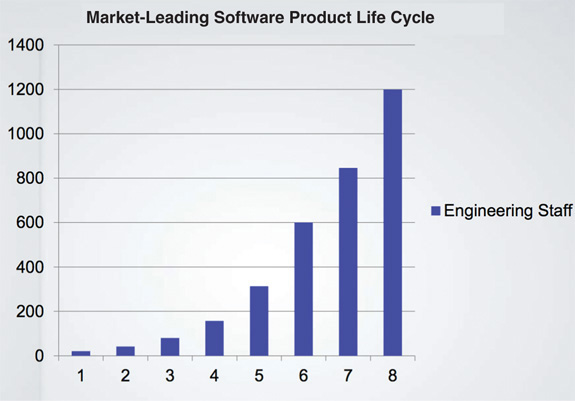
\includegraphics[width=0.8\linewidth]{images/EA/diagram_growth_of_staff.jpg}
    \caption{Personalzuwachs \\ \cite[S. 5]{EA:Book01}}
    \label{fig:personnel-growth}
\end{figure}

In der Abbildung \ref{fig:personnel-growth} wird dargestellt, wie der Personalaufwand im Laufe der Zeit ansteigt.
Das Balkendiagramm zeigt dabei, wie viele Ingenieur/innen an einem bestimmten Release beteiligt sind.

Ein Personalzuwachs muss grundsätzlich nicht negativ sein. Allerdings kann eine zunehmend komplexe und schwer veränderbare Architektur dazu führen, dass immer mehr Personal benötigt wird, um die Software zu warten und weiterzuentwickeln. 
Eine solche Entwicklung geht häufig mit einer sinkenden Produktivität des Teams einher, da die steigende Komplexität die Effizienz beeinträchtigt und die Implementierung neuer Funktionen erschwert.

\clearpage

\begin{figure}[H]
    \centering
    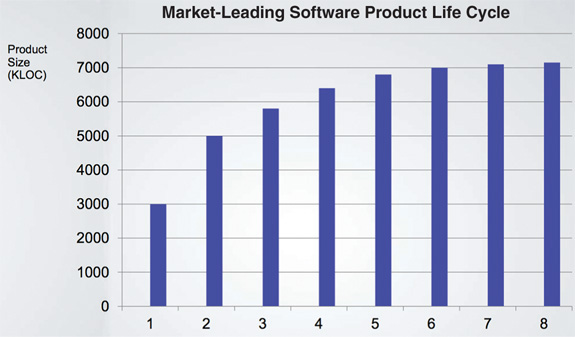
\includegraphics[width=0.8\linewidth]{images/EA/diagram_productivity.jpg}
    \caption{Produktivität \\ \cite[S. 6]{EA:Book01}}
    \label{fig:productivity}
\end{figure}

Betrachtet man anschließend die Abbildung \ref{fig:productivity}, wird die oben genannte Problematik deutlich.
Die Produktivität wird hier anhand der geschriebenen Codezeilen gemessen, was zwar wenig darüber aussagt, ob tatsächlich neue Funktionen oder Änderungen erfolgreich umgesetzt wurden. Mehr Code bedeutet schließlich nicht zwangsläufig, dass dadurch bessere Ergebnisse erzielt werden.

Zu Beginn scheint die Produktivität zwar zu steigen, nähert sich jedoch ab einem gewissen Punkt einer Asymptote\footnote{Linie, der sich eine Kurve immer weiter annähert, ohne sie jemals zu berühren}. Das bedeutet, dass das Hinzufügen weiterer Ressourcen nicht automatisch zu einer Steigerung der Produktivität führt. 

Das Problem dabei ist nicht nur, dass das Unternehmen weitere Personen einstellen und bezahlen muss, sondern auch, dass die derzeitigen Mitarbeiter/innen darunter leiden könnten. Eine abnehmende Produktivität kann zu \textbf{Motivationsverlust} führen, sodass Mitarbeitende im schlimmsten Fall sogar das Unternehmen verlassen. 
\cite[S. 5-10]{EA:Book01} 

\begin{figure}[H]
    \centering
    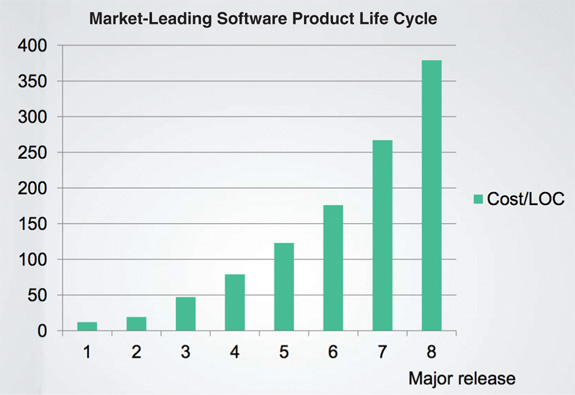
\includegraphics[width=0.7\linewidth]{images/EA/diagram_costs.jpg}
    \caption{Kostenentwicklung \\ \cite[S. 7]{EA:Book01}}
    \label{fig:cost-development}
\end{figure}

Ein Blick auf die Entwicklung der Kosten in Abbildung \ref{fig:cost-development} zeigt, dass die Kosten trotz kaum ansteigender Produktivität (siehe Abbildung \ref{fig:productivity}) und steigendem Personalbedarf (siehe Abbildung \ref{fig:personnel-growth}) immer weiter steigen. Dies bedeutet, dass der \textbf{Kunde oder die Kundin enorme Summen für kaum sichtbare Fortschritte investiert}. 

Ist der Kunde oder die Kundin nicht gewillt, dafür zu bezahlen, kann dies zum Abbruch des Projekts führen, wodurch das Unternehmen in ein schlechtes Licht gerückt wird und im schlimmsten Fall mit der Auflösung des Unternehmens enden kann. \\
\cite[S. 5-10]{EA:Book01} 

% --- Ü B E R L E I T U N G   Z U R   A N F O R D E R U N G S A N A L Y S E ---

All diese Probleme können durch eine \glqq gute\grqq\ Softwarearchitektur vermieden werden. Doch was versteht man darunter? Was ist gut und was ist schlecht? Fakt ist, dass es keine universelle Lösung für die Softwarearchitektur gibt. Abhängig vom Anwendungsfall, Anforderungen, Teamgröße und vielen weiteren Faktoren kann eine andere Architektur vorteilhaft sein.
Im weiteren Verlauf wird näher auf die Anforderungen einer Software eingegangen, die notwendig sind, um einen passenden Architekturstil auszuwählen.


    \clearpage

    \section{Anforderungsanalyse} \label{Anforderungsanalyse}
    % --- E I N L E I T U N G ---

Nachdem in der Einleitung \ref{Allgemeines} ausführlich erläutert wird, warum eine durchdachte Softwarearchitektur von so großer Bedeutung ist, wird anschließend detaillierter auf die Anforderungen einer Software eingegangen. Diese sind entscheidend für den Erfolg eines Softwaresystems.

Grundsätzlich wird angenommen, dass Anforderungen dazu dienen, ein spezifisches Problem zu lösen.
Diese Definition lässt sich auch auf die Anforderungen eines Softwaresystems übertragen. \\ 
Der IEEE-Standard 729 definiert Softwareanforderungen folgendermaßen: 

\begin{quote}
    ``A condition or capability needed by a user to solve a problem or achieve an objective.``
    \cite{EA:Web05}
\end{quote}

Anforderungen werden von verschiedenen Beteiligten wie Benutzern, Kunden, Entwicklern und Business Analysts definiert.

Zusammengefasst dienen Anforderungen dazu, festzulegen, \textbf{welche Probleme die zu entwickelnde Software lösen soll}. Die daraus gewonnen Informationen geben allen Beteiligten einen einheitlichen Überblick und dienen als Entscheidungsgrundlage für einen Architekturstil. 
Allerdings kann es vorkommen, dass die gewählte Architektur zu einem späteren Zeitpunkt nicht mehr optimal ist, da im Laufe des Projekts unerwartete Probleme auftreten können. \\
\cite{EA:Web04, EA:Web05} \cite[S. 13-16]{EA:Book02}

Dies ist besonders relevant bei \textbf{agilen Vorgehensweisen}, bei denen die Zufriedenheit des Kunden im Vordergrund steht. 
\textbf{Laufende Anpassungen} werden vorgenommen, um den Erwartungen des Kunden gerecht zu werden, was bedeutet, dass sich die Anforderungen im Laufe der Zeit ändern können.
\cite{EA:Web06}

Grundsätzlich lassen sich Anforderungen in zwei Haupttypen unterteilen:

\begin{itemize}
    \item Funktionale Anforderungen
    \item Nicht-funktionale Anforderungen
\end{itemize}

Diese werden im Folgenden genauer erklärt. Anschließend erfolgt eine Anforderungsanalyse für das Projekt CGM MAXX LITE,
die dabei helfen soll, einen passenden Architekturstil für das Projekt zu finden, um die Entwicklung, Bereitstellung und Wartung so einfach und kostengünstig wie möglich zu gestalten.


% --- F U N K T I O N A L E   A N F O R D E R U N G E N ---

\subsection{Funktionale Anforderungen} \label{Funktionale Anforderungen}

Der Begriff \glqq funktionale Anforderungen\grqq\ deutet bereits darauf hin, dass es um die konkrete Funktionalität der Software geht. Diese Anforderungen definieren, \textbf{welche Aufgaben ein System erfüllen muss}. Genauer gesagt handelt es sich um sichtbare Funktionen und Prozesse, die der Benutzer sehen und verwenden kann. Der Benutzer führt bestimmte Aktionen durch, die eine festgelegte Operation auslösen und als Antwort eine entsprechende Reaktion des Systems liefern.

Da funktionale Anforderungen immer spezifisch auf die zu entwickelnde Software zugeschnitten sind, \textbf{können} sie \textbf{je nach Projekt stark variieren}. Der genaue Inhalt dieser Anforderungen hängt davon ab, welche Ziele die Software verfolgt und welche Probleme sie lösen soll. Im Abschnitt \ref{Projektbezug - Anforderungsanalyse} wird näher auf die funktionalen Anforderungen des Softwareprojekts CGM MAXX LITE eingegangen.

Funktionale Anforderungen werden im \textbf{agilen Entwicklungsprozess} häufig in Form von \textbf{User Stories} formuliert. Diese beschreiben aus der Perspektive einer bestimmten Rolle, welche Funktionen umgesetzt werden sollen.
\cite{EA:Web04, EA:Web07}


% --- N I C H T - F U N K T I O N A L E   A N F O R D E R U N G E N ---

\subsection{Nicht-funktionale Anforderungen} \label{Nicht-funktionale Anforderungen}

Neben den funktionalen Anforderungen gibt es auch die nicht-funktionalen Anforderungen, die auch als architektonische Eigenschaften bezeichnet werden. Dabei handelt es sich um bestimmte Kriterien, die erfüllt sein müssen, \textbf{damit ein Softwaresystem erfolgreich betrieben werden kann}.

Grundsätzlich werden diese Anforderungen in bestimmten Dokumenten angeführt. Allerdings gibt es einige Eigenschaften, welche zwar essentiell für den Projekterfolg sind, aber nicht explizit genannt werden, da davon ausgegangen wird, dass die Software verfügbar, verlässlich und sicher ist.

Diese Anforderungen können für die unterschiedlichsten Bereiche der Software definiert werden.
Um ein besseres Verständnis für die verschiedenen Eigenschaften zu bekommen, können diese in Kategorien unterteilt werden.
Anzumerken ist, dass es hierbei ebenfalls keine allgemein gültige Aufteilung gibt. 

Allerdings ist es nahezu unmöglich, all diese Anforderungen wirklich zu erfüllen, da sich die einzelnen Eigenschaften gegenseitig beeinflussen können. \\
\cite{EA:Web04, EA:Web05} \cite[S. 55-60]{EA:Book02}


    % --- B E T R I E B S R E L E V A N T E   A N F O R D E R U N G E N ---
    
    \subsubsection{Betriebsrelevante Anforderungen}
    
    Für den Betrieb einer Software sind bestimmte Eigenschaften von großer Bedeutung. Dazu zählt insbesondere die \textbf{Verfügbarkeit}, die angibt, wann und wie lange das System zur Verfügung stehen muss und welche Maßnahmen im Falle eines Ausfalls ergriffen werden. Ein weiterer wichtiger Aspekt ist die \textbf{Performance}, die durch die maximale Antwortzeit\footnote{Zeitspanne zwischen Aktion eines Nutzers und der Antwort des Systems} definiert wird.
    Hierbei muss berücksichtigt werden, dass die Reaktionszeit der Applikation je nach Nutzung und Anzahl der Benutzer stark variieren kann. Besonders in Systemen mit einer hohen Benutzerzahl kann es zu Verzögerungen kommen.
    
    Weitere wesentliche Aspekte sind die \textbf{Wiederherstellbarkeit, Verlässlichkeit und die Sicherheit} des Systems.
    Vor allem bei Applikationen, bei denen Menschenleben gefährdet werden könnten, ist besondere Vorsicht geboten.
    Es muss nicht zwangsläufig ein vollständiger Systemausfall vorliegen. Alleine das bloße Fehlen oder der Verlust von wichtigen Informationen kann zu ernsthaften Komplikationen führen. \\
    Grundsätzlich sollte bei jeder Software auf Sicherheit geachtet werden, um unbefugten Zugriff zu verhindern. 
    Der potenzielle Schaden steigt mit der Anzahl der Nutzer, die auf das System zugreifen, sowie mit der Menge an verwalteten Daten. Dies gilt insbesondere für sensible und personenbezogene Daten. \\
    \cite[S. 58-59]{EA:Book02} \cite{EA:Web08}
    
    Aus diesem Grund ist es sinnvoll, bereits in der Anforderungsanalyse die Wiederherstellbarkeit des Systems zu berücksichtigen. Klare Anforderungen, die definieren, wie das System im Falle eines Ausfalls oder Fehlers reagieren soll, helfen, die Software schnell und effektiv wiederherzustellen. Diese Maßnahmen tragen dazu bei, die Zuverlässigkeit des Systems zu gewährleisten und es auch nach Störungen weiterhin funktionsfähig zu halten.
    \cite{EA:Web09}
    
    
    % --- S T R U K T U R E L L E   A N F O R D E R U N G E N ---
    
    \subsubsection{Strukturelle Anforderungen}
    
    Auch der Code darf nicht außer Acht gelassen werden, weshalb Kriterien festgelegt werden, um die Qualität der Software sicherzustellen. Dazu gehören Eigenschaften wie die \textbf{Erweiterbarkeit}, die eine wichtige Rolle spielt, wenn das System in Zukunft um weitere Funktionen ergänzt werden soll.
    
    Die \textbf{Wiederverwendbarkeit} bestimmter Komponenten kann in einigen Anwendungsfällen von Bedeutung sein, ebenso wie die \textbf{Lokalisierung\footnote{Unterstützung verschiedener Sprachen, Maßeinheiten und Währungen}} für größere Unternehmen, die in mehreren Ländern tätig sind.
    
    Wie bereits im Abschnitt \ref{Herausforderungen und Probleme} erwähnt, muss auch die \textbf{Wartung} berücksichtigt werden, um die Kosten niedrig zu halten. Dabei muss überlegt werden, wie Änderungen effizient umgesetzt werden können, um das System zu verbessern.
    
    Bei der Entwicklung eines Prototyps kann es ebenfalls wichtig sein, die \textbf{Portabilität} zu beachten, speziell dann, wenn Teile der Software in ein bereits bestehendes System integriert werden sollen, das auf einer anderen Technologie basiert. \\
    \cite[S. 59-60]{EA:Book02}
    
    
    % --- B E R E I C H S Ü B E R G R E I F E N D E   A N F O R D E R U N G E N ---
    
    \subsubsection{Bereichsübergreifende Anforderungen}
    
    Es gibt viele weitere Kriterien, die das Design der Software maßgeblich beeinflussen können.
    Dazu gehören die \textbf{Zugänglichkeit} in Bezug auf Barrierefreiheit, sowie bestimmte Sicherheitsaspekte wie die \textbf{Authentifizierung und Autorisierung}.
    Auch \textbf{rechtliche Aspekte} müssen berücksichtigt werden, etwa die Datenschutz-\\Grundverordnung (DSGVO).
    Zudem spielt \textbf{Usability} eine große Rolle, damit die Anwender/innen bedenkenlos mit der Software arbeiten können, ohne viel Zeit damit zu verbringen, nach den verfügbaren Funktionalitäten zu suchen. \\
    \cite[S. 60]{EA:Book02}
    
    
    % --- Ü B E R L E I T U N G ---
    
    \subsubsection{Überleitung}
    
    Im folgenden Abschnitt werden die Anforderungen des Projekts CGM MAXX LITE genauer analysiert.
    Hierbei werden sowohl die Erwartungen des Auftraggebers, wie sie im Pflichtenheft festgelegt sind, als auch die aus der Anwendersicht formulierten Anforderungen, die als User Stories in Jira dokumentiert sind, berücksichtigt.
    Ziel ist es, die Eigenschaften zu definieren, die das System schlussendlich erfüllen soll, um sowohl den Auftraggeber zufriedenzustellen als auch den Anforderungen der Anwender/innen gerecht zu werden.
    Außerdem sollen die daraus gewonnenen Erkenntnisse als Entscheidungsgrundlage für die Auswahl eines Architekturstils dienen, worauf im Unterkapitel \ref{Architekturstile} näher eingegangen wird.
    
    \clearpage


% --- P R O J E K T B E Z U G ---

\subsection{Projektbezug - Anforderungsanalyse} \label{Projektbezug - Anforderungsanalyse}

Bevor die Anforderungen des Projekts CGM MAXX LITE genauer unter die Lupe genommen werden, muss zunächst die Frage geklärt werden, worum es sich hierbei überhaupt handelt. Alle Informationen, die in diesem Abschnitt genannt werden, stammen von der Website des Auftraggebers, aus dem Pflichtenheft und den User Stories und Tasks in Jira.
Im Folgenden wird beschrieben, wie der Projektauftrag zustande kam und was genau durch dieses Projekt erreicht werden soll. 


% --- A U S G A N G S S I T U A T I O N ---

\subsubsection{Ausgangssituation}

Der Name verrät bereits, von welchem Unternehmen der Projektauftrag stammt. Dieses heißt \textbf{CGM Arztsysteme Österreich GmbH} und ist spezialisiert auf Software im Gesundheitssektor. Dabei ist \textbf{CGM MAXX} eines ihrer Hauptprodukte, ein Arztinformationssystem, das sowohl von Wahl- als auch von Kassenärzten genutzt wird.

Um etwas genauer zu sein, handelt es sich um eine webbasierte Arztsoftware, die diversen Ärzten digitale Dienste zur Verfügung stellt, wie die Patientenverwaltung, Befund-Dokumentierung, Terminplanung und vieles mehr.
Allerdings ist diese Applikation \textbf{nur für den Desktop-Betrieb optimiert} und basiert auf veralteten Technologien.
\cite{EA:Web10}


% --- S O L L - S I T U A T I O N ---

\subsubsection{Soll-Situation}

Hier setzt das Projekt \textbf{CGM MAXX LITE} an. Ziel ist es, die Anwendung auch \textbf{auf mobilen Geräten} wie Smartphones und Tablets bereitzustellen, um \textbf{alltägliche Arbeitsabläufe zu erleichtern}.

Dabei soll ein Prototyp für ein mobiles Frontend entwickelt werden, das die wichtigsten Funktionalitäten von CGM MAXX enthält und zusätzlich Funktionen zur Foto- und Audioaufnahme bietet, um die Vorzüge mobiler Geräte zu nutzen.
Durch die Bereitstellung einer Swagger-Dokumentation, die die einzelnen Schnittstellen der vorhandenen Software genau beschreibt, soll ein Demo-Backend implementiert werden, damit dieses gegebenenfalls mit dem bereits bestehenden Backend von CGM MAXX ausgetauscht und getestet werden kann. \\
Der Fokus liegt dabei auf einer \textbf{benutzerfreundlichen Oberfläche für mobile Endgeräte}. Zudem soll die Software so gestaltet werden, dass sie für zukünftige Erweiterungen offen bleibt, um die Weiterentwicklung und Wartung möglichst effizient und kostengünstig zu gestalten.


    % --- F U N K T I O N A L E   A N F O R D E R U N G E N ---

    \subsubsection{Funktionale Anforderungen}
    
    Was genau unter funktionalen Anforderungen zu verstehen ist, kann im Abschnitt \ref{Funktionale Anforderungen} nachgelesen werden.
    Kurz gesagt geht es darum, welche Funktionalitäten die Software bieten soll. Zur Definition der funktionalen Anforderungen werden die User Stories und Tasks aus Jira herangezogen.
    
    Da es zu unübersichtlich wäre, jede einzelne User Story und jeden Task aufzulisten, folgt eine kurze Übersicht der Funktionalitäten, die die Software grundsätzlich erfüllen soll:
    \begin{itemize}
        \item Dark-/Light Mode
        \item Patientenliste
        \item Patientensuche
        \item Aufnahme und Darstellung von Bildern
        \item Aufnehmen und Abspielen von Audiodateien
    \end{itemize}
    
    Da diese Auflistung noch zu ungenau ist, um ein klares Bild zu vermitteln, werden die grundlegenden Funktionalitäten der zu entwickelnden Software nun näher beschrieben.
    
    Sobald die Applikation gestartet wird, soll eine \textbf{Liste der Patient/innen angezeigt} werden, die am heutigen Tag einen Termin haben. Dies ermöglicht es dem/der Anwender/in, schnell an Informationen zu gelangen, ohne lange suchen zu müssen. \\
    Des Weiteren soll es möglich sein, \textbf{Personen anhand ihres Namens oder ihrer Sozialversicherungsnummer zu suchen}. Diese können auf der Startseite angepinnt werden, falls öfter auf die Daten einer bestimmten Person zugegriffen werden muss. \\ 
    Ein weiterer wichtiger Aspekt ist eine \textbf{Navigationsleiste}, die es dem/der Anwender/in ermöglicht, schnell durch die Applikation zu navigieren. Sie soll so platziert sein, dass sie einfach mit einer Hand erreicht werden kann, um die Benutzerfreundlichkeit zu erhöhen. \\
    Wie bereits erwähnt, sollen die Vorteile mobiler Geräte genutzt werden, weshalb es möglich sein soll, \textbf{Bilder von medizinischen Befunden} direkt \textbf{in der Patientenakte} zu \textbf{hinterlegen}. Dadurch kann sich der/die Arzt/Ärztin auf den/die Patient/in konzentrieren, ohne zu viel Zeit mit administrativen Aufgaben zu verbringen. \\
    Neben Fotos sollen auch \textbf{Audioaufnahmen gespeichert} werden können. Hierbei können Sitzungen aufgezeichnet werden, die in Zukunft genutzt werden können, um die wichtigsten Informationen mithilfe einer KI zu extrahieren und in kurzen Worten zusammenzufassen. 


    % --- N I C H T - F U N K T I O N A L E   A N F O R D E R U N G E N ---

    \subsubsection{Nicht-funktionale Anforderungen}

    Nicht-funktionale Anforderungen definieren Kriterien, die ein System erfüllen muss, um den Anforderungen der Nutzerinnen und Nutzer sowie den Qualitätsansprüchen des Projekts gerecht zu werden. 
    Detaillierte Informationen hierzu sind im Abschnitt \ref{Nicht-funktionale Anforderungen} zu finden.

    Mit Ausnahme der \textbf{Benutzerfreundlichkeit} wurden vom Auftraggeber keine weiteren nicht-funktionalen Anforderungen festgelegt. Dennoch gibt es bestimmte Eigenschaften, die vor allem bei medizinischen Anwendungen, von besonderer Bedeutung sind.
    Ein zentraler Aspekt ist die \textbf{Performance}, die sicherstellen soll, dass alle Arbeitsabläufe reibungslos und ohne signifikante Verzögerungen ablaufen. Darüber hinaus ist die \textbf{Vertraulichkeit} von personenbezogenen Daten essenziell, um den Schutz sensibler Informationen zu gewährleisten wird. 
    Ein weiterer wichtiger Faktor ist die \textbf{Ausfallsicherheit}. Insbesondere bei Applikationen, deren Funktionalität potenziell Auswirkungen auf die Sicherheit oder das Wohlbefinden von Menschen hat, muss sichergestellt werden, dass bei einem Fehler nicht das gesamte System abstürzt, sondern nur betroffene Teile.

    In Bezug auf die Benutzerfreundlichkeit sollten folgende Punkte berücksichtigt werden:
    \begin{itemize}
        \item Eine leicht verständliche und selbsterklärende Benutzeroberfläche
        \item Der/die Anwender/in soll auf bestehende Probleme hingewiesen werden
        \item Arbeitsabläufe sollen mit minimalem Aufwand erledigt werden können
        \item Verwendung eines einheitlichen und schlichten Farbschemas
    \end{itemize}
    

    \clearpage

    \section{Architekturstile} \label{Architekturstile}
    % --- A R C H I T E K T U R S T I L E ---

Wie in Abschnitt \ref{Softwarearchitektur} beschrieben, umfasst die Softwarearchitektur sowohl die Struktur eines Systems als auch die einzelnen Details seiner Umsetzung. Die Anforderungen eines Softwaresystems variieren je nach Art der Anwendung, weshalb unterschiedliche Ansätze erforderlich sind.

Im Laufe der Zeit haben sich bestimmte \glqq{Muster}\grqq\ etabliert, die als Architekturstile bezeichnet werden. 
Benannt werden diese nach bestimmten architektonischen Eigenschaften, die Aufschluss über die Topologie oder potenzielle Herausforderungen geben.

Die Wahl eines geeigneten Architekturstils ist von entscheidender Bedeutung, da sie die grundlegende Struktur des Systems festlegt und den Entwickler/innen als Leitfaden dient. Zudem wird vermieden, dass ein \textbf{\glqq{Big Ball of Mud\footnote{Anti-Pattern, bei dem keine erkennbare Softwarearchitektur existiert}}\grqq}\ entsteht. 

Für eine fundierte Entscheidung wird die Anforderungsanalyse \ref{Projektbezug - Anforderungsanalyse} herangezogen, die festlegt, welche Aspekte besonders relevant sind. 

Ein paar gängige Beispiele:
\begin{itemize}
    \item Monolithische Architektur
    \item Serviceorientierte Architektur (SOA)
    \item Eventbasierte Architektur
    \item Serverlose Architektur
    \item Microservices-Architektur
\end{itemize}

Um den Fokus auf cloudbasierte Systeme zu richten, wird im Anschluss eine Auswahl relevanter Architekturstile beschrieben, die in modernen Cloud-Umgebungen besonders häufig Anwendung finden. 
\cite[S. 125-126]{EA:Book02} \cite{EA:Web60}


\clearpage


    % --- M I C R O S E R V I C E   A R C H I T E K T U R ---

    \subsection{Microservices-Architektur} \label{Microservices-Architektur}

    Die nach Fowler und Lewis benannte \glqq{Microservices-Architektur}\grqq\ ist einer der am häufigsten eingesetzten Architekturstile der heutigen Zeit. Besonders in den letzten Jahren hat dieser Architekturstil stark an Bedeutung gewonnen.

    Dabei wird nicht eine große Applikation entwickelt, die als eine Einheit bereitgestellt werden kann, sondern mehrere voneinander unabhängige Services, die miteinander interagieren und so ein System bilden. Es handelt sich um eine \textbf{verteilte Architektur}.
    Die Unterteilung in die einzelnen Komponenten erfolgt anhand des \textbf{Domain-Driven-Designs (DDD)}.
    \cite[S. 251-253]{EA:Book02}

    Ziel ist es, die grundlegenden Komponenten des Systems eigenständig zu betreiben, sodass im Falle eines Fehlers nur ein Dienst ausfällt und nicht das gesamte System. 
    \cite{EA:Web61}

        % --- A U F B A U ---
    
        \subsubsection{Aufbau}
    
        In Abbildung \ref{fig:microservices-topology} wird dargestellt, wie der allgemeine Aufbau einer Microservices-Architektur aussieht:
    
        \begin{figure}[H]
            \centering
            
\includegraphics[width=0.45\linewidth]{images/EA/microservices-topology.png}
            \caption{Microservices Topologie \\ \cite[S. 252]{EA:Book02}}
            \label{fig:microservices-topology}
        \end{figure}

        Grundsätzlich gibt es eine zentrale API-Schnittstelle, die die Anfragen der Clients an die entsprechenden Microservices weiterleitet.
        Bestehen Abhängigkeiten zwischen den Diensten, erfolgt die Kommunikation ebenfalls über die gemeinsame Schnittstelle.
        \cite{EA:Web61}

        Eine dedizierte Datenbank pro Service soll dabei für \textbf{Fehlertoleranz} sorgen, sodass, wie vorhin bereits erwähnt, nur die vom Fehler betroffenen Teile des Systems ausfallen, während andere Dienste und Daten weiterhin verfügbar bleiben.
        \cite[S. 268]{EA:Book02}

        Da es sich hierbei um einen cloudnativen Ansatz handelt, ist es üblich, moderne Methoden wie \textbf{DevOps} (siehe Abschnitt \ref{DevOps}) zu verwenden, um Software einfach und schnell zu entwickeln und in der Cloud bereitzustellen (siehe Unterkapitel \ref{Cloud Computing}). 
        Um dies zu ermöglichen, ist es oft notwendig, die Organisation so umzustrukturieren, dass sie in mehrere kleine Teams unterteilt wird, die für unterschiedliche Dienste verantwortlich sind. In der Theorie bietet dies den Vorteil, dass durch die unabhängigen Dienste weniger oder gar keine Konflikte mehr auftreten und die Auslieferung somit schneller erfolgen kann.
        \cite{EA:Web62}

        % --- V O R -   U N D   N A C H T E I L E ---

        \subsubsection{Vor- und Nachteile}

        Die Microservices-Architektur bietet dabei einige Vor- und Nachteile, die tabellarisch in \ref{tab:microservices-pros-and-cons} dargestellt werden. Bei einer gut durchdachten Umsetzung können einige der aufgelisteten Nachteile vermieden werden. \\
        \cite[S. 253, 268-269]{EA:Book02} \cite{EA:Web62} \\

        \begin{table}[H]
            \centering
            \begin{tabular}{|p{7.5cm}|p{7.5cm}|}
                \hline
                \cellcolor{green!40} \textbf{Vorteile} & \cellcolor{red!40} \textbf{Nachteile} \\ \hline
                 + Unterstützung agiler Vorgehensweisen & - Netzwerkbedingte Performanceverluste \\
                 + Hohe Fehlertoleranz & - Komplexer Aufbau \\ 
                 + Flexible Skalierung & - Erschwertes Testen \& Debuggen \\
                 + Einfache Wartung \& Erweiterbarkeit & - Erhöhter Ressourcenbedarf \\
                 \hline
            \end{tabular}
            \caption{Vor- und Nachteile der Microservices-Architektur}
            \label{tab:microservices-pros-and-cons}
        \end{table}


        % --- E I N S A T Z G E B I E T E ---

        \subsubsection{Einsatzgebiete}

        Unternehmen, die eine Vielzahl unterschiedlicher Dienste über das Internet bereitstellen, profitieren von den Vorteilen der Microservices-Architektur. Diese hat nicht nur einen positiven Einfluss auf die Softwareentwicklung, sondern optimiert auch die Nutzererfahrung. \\
        Denn durch die flexible Skalierung einzelner Applikationen lassen sich Engpässe durch gezieltes Hinzufügen oder Entfernen von Ressourcen effektiv vermeiden.
        \cite{EA:Web62}

        Folgende Beispiele verdeutlichen die Relevanz der Microservices-Architektur:
        \begin{itemize}
            \item \textbf{Social-Media-Plattformen}
            \begin{itemize}[label=$\circ$]
                \item z.B. Instagram, Facebook, X, usw.
            \end{itemize}

            \item \textbf{Video-Streaming-Dienste} 
            \begin{itemize}[label=$\circ$]
                \item z.B. Netflix, Amazon Prime, usw.
            \end{itemize}
            
            \item \textbf{E-Commerce-Webseiten}
            \begin{itemize}[label=$\circ$]
                \item z.B. eBay, Amazon, usw.
            \end{itemize}
        \end{itemize}


    % --- E V E N T G E S T E U E R T E   A R C H I T E K T U R ---
    
    \subsection{Eventbasierte Architektur} \label{Eventbasierte Architektur}

    Ein weiterer Architekturstil, der oft im Zusammenhang mit der Microservices-Architektur eingesetzt wird, ist der \textbf{eventbasierte Architekturstil}. Ähnlich wie bei der Microservices-Architektur ist auch dies eine verteilte Architektur, bei der die \textbf{Kommunikation} zwischen den einzelnen Bestandteilen des Systems \textbf{asynchron\footnote{Senden/Empfangen von Daten ist zeitlich versetzt}} abläuft. \\
    \cite[S. 183]{EA:Book02}

    Wie bei anderen Architekturstilen gibt es verschiedene Möglichkeiten zur Umsetzung. In diesem Fall unterscheidet man zwischen \textbf{zwei Mustern}, die zur Realisierung einer eventbasierten Architektur genutzt werden:
    \begin{itemize}
        \item \textbf{Publisher \& Subscriber}
        \begin{itemize}[label=$\circ$]
            \item Subscriber erhalten Benachrichtigungen von den abonnierten Kanälen und reagieren darauf.  
        \end{itemize}
        
        \item \textbf{Event Streaming}
        \begin{itemize}[label=$\circ$]
            \item Subscriber können den gesamten Stream lesen
            \item Nur die für den Subscriber relevanten Informationen werden verarbeitet
        \end{itemize}
    \end{itemize}

    \cite{EA:Web63}


         % --- A U F B A U ---
    
        \subsubsection{Aufbau}

        Abbildung \ref{fig:event-driven-architecture-topology} stellt dabei eine Form der eventgesteuerten Architektur dar.

        \begin{figure}[H]
            \centering
            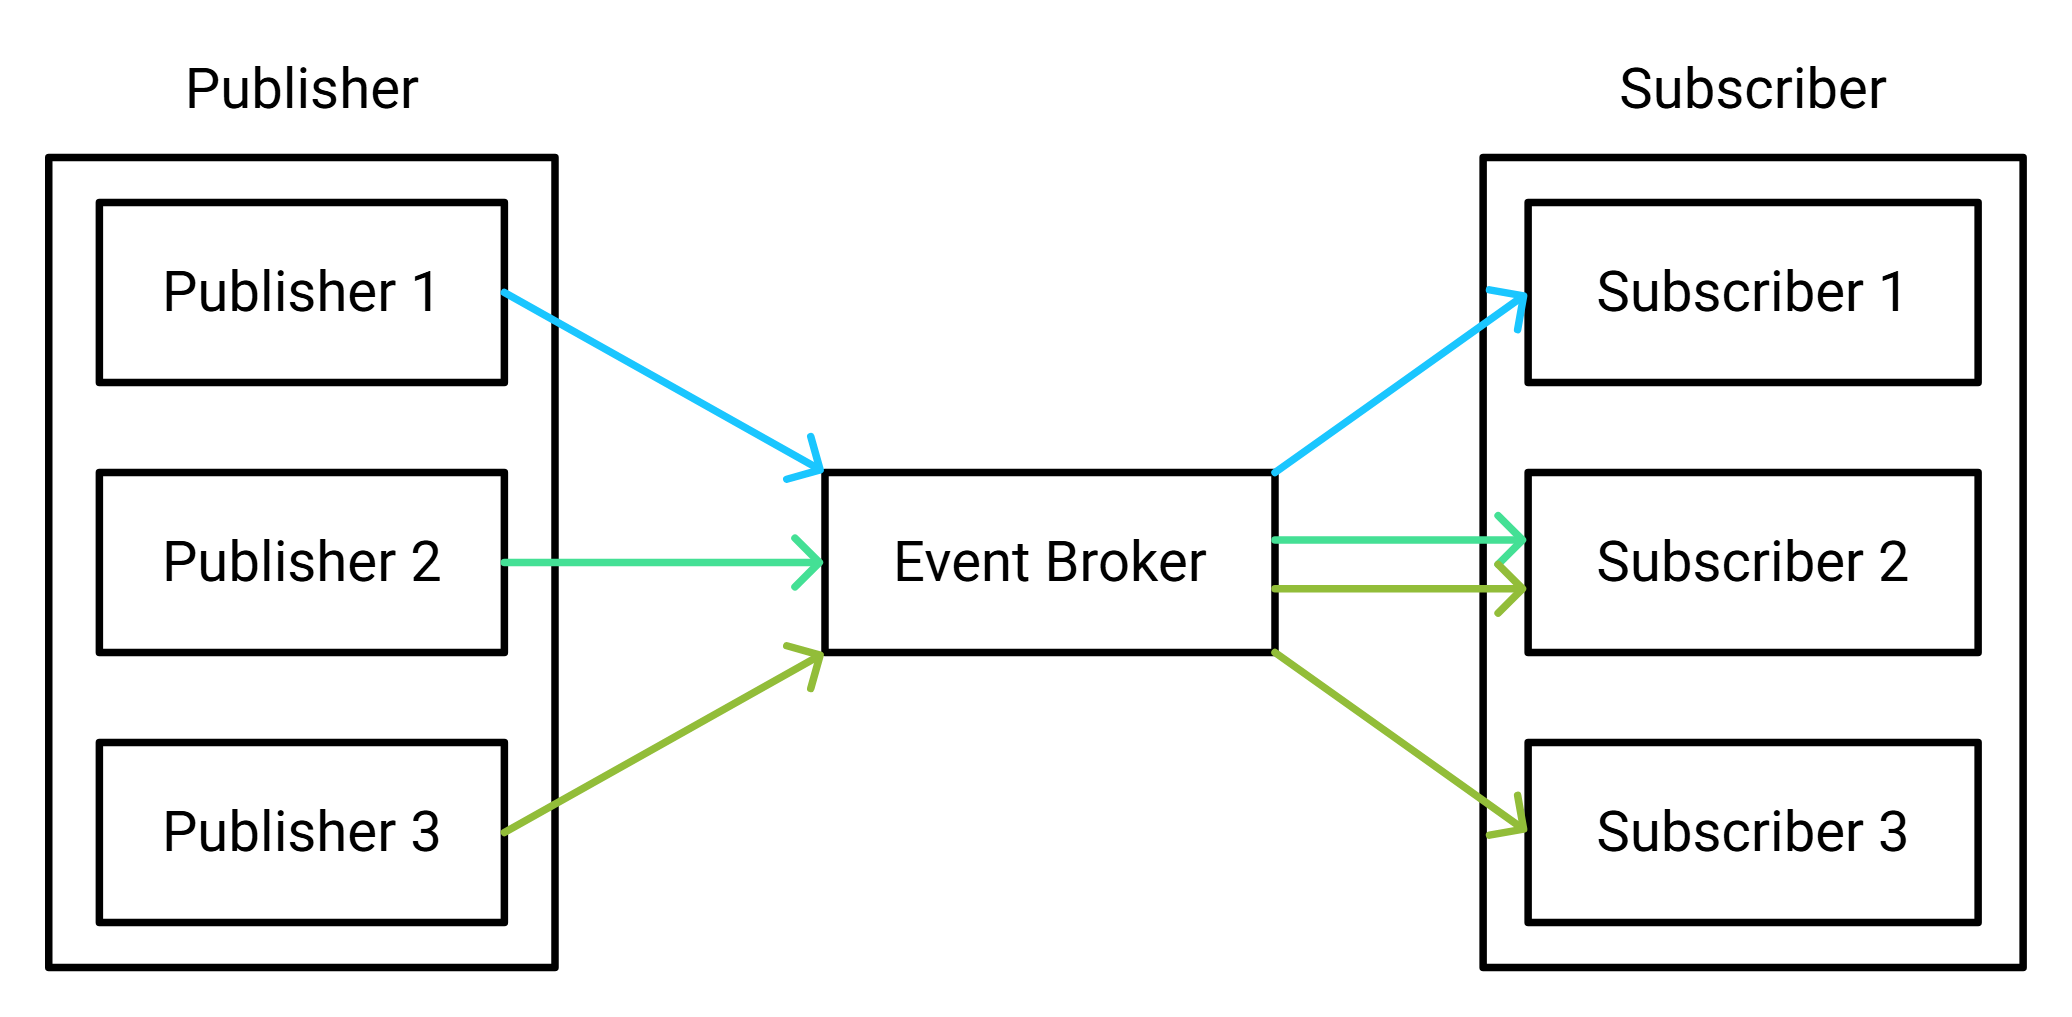
\includegraphics[width=0.9\linewidth]{images/EA/even-driven-architecture.png}
            \caption{Eventbasierte Architektur - Publisher/Subscriber \\ \cite{EA:Img02}}
            \label{fig:event-driven-architecture-topology}
        \end{figure}

        Das Publisher/Subscriber-Muster besteht aus folgenden Bestandteilen:
        \begin{itemize}
            \item \textbf{Publisher}
            \begin{itemize}[label=$\circ$]
                \item Lösen Ereignisse aus und senden diese an den Event Broker
                \item z.B. Bedienung einer Benutzeroberfläche 
            \end{itemize}
            
            \item \textbf{Subscriber}
            \begin{itemize}[label=$\circ$]
                \item Konsumieren und verarbeiten Ereignisse
                \item Empfangen Ereignisse abonnierter Event Channels des Brokers
            \end{itemize}
            
            \item \textbf{Broker}
            \begin{itemize}[label=$\circ$]
                \item Kümmert sich um die richtige Weiterleitung der Ereignisse
            \end{itemize}
        \end{itemize}

        \cite{EA:Web63}
        
        \clearpage
        
        % --- V O R -   U N D   N A C H T E I L E ---
    
        \subsubsection{Vor- und Nachteile}

        Die eventbasierte Architektur bietet einige Vor- und Nachteile:
    
        \begin{table}[H]
            \centering
            \begin{tabular}{|p{7.5cm}|p{7.5cm}|}
                \hline
                \cellcolor{green!40} \textbf{Vorteile} & \cellcolor{red!40} \textbf{Nachteile} \\ \hline
                 + Hohe Fehlertoleranz & - Erschwertes Testen \& Debuggen \\
                 + Hohe Performance & - Risiko von Datenverlusten \\ 
                 + Hohe Skalierbarkeit & - Komplexer Ablauf \& Implementierung \\
                 + Einfache Erweiterbarkeit & - Schwierige Fehlerbehandlung \\
                 + Echtzeitunterstützung & ~ \\
                \hline
            \end{tabular}
            \caption{Vor- und Nachteile der eventbasierten Architektur}
            \label{tab:event-driven-architecture-pros-and-cons}
        \end{table}

        Da dieser Architekturstil ebenfalls auf den Konzepten verteilter Systeme basiert, bietet er ähnliche Vorteile wie die Microservices-Architektur. Zudem eignet sich die ereignisgesteuerte Architektur für Echtzeit-Anwendungen, da sofort auf eintretende Ereignisse reagiert werden kann.
        
        Allerdings bringt die asynchrone Kommunikation einige Herausforderungen mit sich. Dazu zählt insbesondere die \textbf{Koordination der einzelnen Events}, sodass deren Reihenfolge erhalten bleibt und ein kontrollierter Ablauf gewährleistet wird. Da Ereignisse dynamisch eintreten, ist es oft schwierig, den genauen Ablauf nachzuvollziehen und mögliche Fehlerquellen zu identifizieren. \\
        \cite[S. 183, S. 205, S. 211-213]{EA:Book02}
    
        % --- E I N S A T Z G E B I E T E ---
    
        \subsubsection{Einsatzgebiete}

        Der eventgesteuerte-Architekturstil hat zahlreiche Anwendungsfälle in den unterschiedlichsten Bereichen.
        Dazu gehören:
        \begin{itemize}
            \item \textbf{Finanzapplikationen}
            \begin{itemize}[label=$\circ$]
                \item z.B. Subscriber informieren, sobald sich der Kurs einer Aktie ändert
            \end{itemize}

            \item \textbf{Internet of Things (IoT)}
            \begin{itemize}[label=$\circ$]
                \item z.B. Überwachung von Sensordaten
            \end{itemize}

            \item \textbf{Software im Gesundheitswesen}
            \begin{itemize}[label=$\circ$]
                \item z.B. Automatische Aktualisierung von Patientendaten
            \end{itemize}
        \end{itemize}

        \cite{EA:Web64} \cite[S. 184]{EA:Book02}

    \clearpage


    % --- S E R V E R L E S S   A R C H I T E K T U R ---
    
    \subsection{Serverlose Architektur}

    Der letzte cloudnative Architekturstil, der im Zuge dieser Arbeit beschrieben wird, ist die \textbf{serverlose Architektur}. 
    Bei dieser Art von Architektur steht weniger der eigentliche Aufbau eines Systems im Vordergrund, sondern die Verwaltung der benötigten Ressourcen. Die serverlose Architektur wird häufig in Kombination mit der Microservices-Architektur (siehe \ref{Microservices-Architektur}) oder der ereignisgesteuerten Architektur (siehe \ref{Eventbasierte Architektur}) eingesetzt. 

    Ziel dieser Architektur ist es, den Fokus der Entwickler/innen auf das Schreiben des eigentlichen Codes zu lenken, ohne sich mit den Anforderungen der für den Betrieb notwendigen IT-Infrastruktur auseinandersetzen zu müssen. Stattdessen übernimmt ein entsprechender Cloud-Dienstanbieter diese Aufgabe, einschließlich der Bereitstellung und Skalierung der Applikationen. Dadurch muss ein Unternehmen \textbf{nur für die tatsächlich verwendeten Rechenressourcen bezahlen}.

    Wird eine bereitgestellte Applikation nicht verwendet, so werden auch keine Ressourcen benötigt. Das heißt, \textbf{Ressourcen werden dynamisch bereitgestellt}.

    Die serverlose Architektur lässt sich dabei in zwei Bereiche eingliedern:
    \begin{enumerate}
        \item \textbf{Backend-as-a-Service (BaaS)}
        \begin{itemize}[label=$\circ$]
            \item Integration von Drittanbieterdiensten und Applikationen möglich
            \item Kommunikation erfolgt über APIs
            \item Auslagerung bestimmter Funktionalitäten - z.B. Authentifizierung
        \end{itemize}
        
        \item \textbf{Function-as-a-Service (FaaS)}
        \begin{itemize}[label=$\circ$]
            \item Ereignisgesteuert
            \item Bereitgestellter Code wird nur bei Aufruf ausgeführt
        \end{itemize}
    \end{enumerate}

    Da es für diesen Architekturstil keine allgemein gültige Topologie gibt, sondern abhängig ist von der eingesetzten Technologie, wird auf die Darstellung des Aufbaus verzichtet. Stattdessen werden Technologien genannt, die für die Umsetzung einer serverlosen Architektur verwendet werden können:
    \begin{itemize}
        \item AWS Lambda
        \item Azure Functions
        \item Google Cloud Functions
    \end{itemize}
    \cite{EA:Web65}
    
    \clearpage

        % --- V O R -   U N D   N A C H T E I L E ---

        \subsubsection{Vor- und Nachteile}

        In Tabelle \ref{tab:serverless-architecture-pros-and-cons} werden die wichtigsten Vor- und Nachteile des serverlosen Architekturstils aufgelistet:
    
        \begin{table}[H]
            \centering
            \begin{tabular}{|p{7.5cm}|p{7.5cm}|}
                \hline
                \cellcolor{green!40} \textbf{Vorteile} & \cellcolor{red!40} \textbf{Nachteile} \\ \hline
                 + Kosteneinsparungen & - Neue Sicherheitsrisiken \\
                 + Erhöhte Produktivität & - Mögliche Einschränkungen \\ 
                 + Hohe Skalierbarkeit & - Erhöhte Latenz \\
                 + Integration von Drittanbietersoftware & - Weniger Kontrollmöglichkeiten \\
                \hline
            \end{tabular}
            \caption{Vor- und Nachteile der serverlosen Architektur}
            \label{tab:serverless-architecture-pros-and-cons}
        \end{table}
        \cite{EA:Web66}
    
         % --- E I N S A T Z G E B I E T E ---
    
        \subsubsection{Einsatzgebiete}

        Wie für die zuvor genannten Architekturstile, kann auch die serverlose Architektur in unzähligen Bereichen eingesetzt werden:
        \begin{itemize}
            \item Backend-Applikationen
            \item Spezielle Aufgaben, die in einem festgelegten Intervall ausgeführt werden
            \begin{itemize}[label=$\circ$]
                \item Berichte generieren
                \item Backup einer Datenbank erstellen
            \end{itemize}
            \item Webapplikationen mit schwer vorhersehbarer Nachfrage
        \end{itemize}
        \cite{EA:Web65}

    \clearpage


    % --- P R O J E K T B E Z U G ---
    
    \subsection{Projektbezug - Architekturstil} \label{Projektbezug - Architekturstil}

    Basierend auf der Anforderungsanalyse (siehe Abschnitt \ref{Projektbezug - Anforderungsanalyse}) wird eine geeignete Architektur für das Projekt ausgewählt. Die folgenden Punkte fassen die für das Projekt CGM MAXX LITE relevanten Anforderungen zusammen:
    \begin{itemize}
        \item \textbf{Funktionale Anforderungen:}
        \begin{itemize}[label=$\circ$]
            \item Patientensuche und Darstellung der zugehörigen Daten
            \item Hinterlegung von Bildern und Audiodateien in der Patientenakte
        \end{itemize}
        
        \item \textbf{Nicht-funktionale Anforderungen:}
        \begin{itemize}[label=$\circ$]
            \item Hohe Ausfallsicherheit
            \item Skalierbarkeit einzelner Komponenten
            \item Erweiterbarkeit für zukünftige Funktionalitäten
        \end{itemize}
    \end{itemize}

    Die funktionalen Anforderungen lassen sich dabei in zwei Bereiche unterteilen:
    \begin{enumerate}
        \item Verwaltung von Patientendaten
        \item Verwaltung von Dateien
    \end{enumerate}

    Unter Berücksichtigung der zuvor beschriebenen Architekturstile (siehe Unterkapitel \ref{Architekturstile}) eignet sich die \textbf{Microservices-Architektur} besonders gut. Zudem ermöglicht sie es, die Software in zwei Subdomänen zu unterteilen. Dadurch lassen sich die Kernfunktionalitäten der Software in zwei unabhängige Services auslagern, was die \textbf{Fehlertoleranz} und \textbf{Wartbarkeit} erhöht.

    Sowohl die ereignisgesteuerte Architektur als auch die Ansätze des serverlosen Computings hätten sich ebenfalls für die Umsetzung von CGM MAXX LITE geeignet. Da der Fokus jedoch auf der Entwicklung der Benutzeroberfläche liegt und der Wunsch des Auftraggebers ist, die Software so zu gestalten, dass anstelle des von uns entwickelten Backends das Backend der Desktop-Applikation CGM MAXX angebunden werden kann, fiel die Entscheidung auf eine einfache Microservices-Architektur.

    Zur Implementierung wird das Java-Framework \textbf{Spring Boot} in Kombination mit der \textbf{Spring Cloud} Library eingesetzt.
    Diese Entscheidung basiert sowohl auf den umfangreichen Funktionalitäten der Technologie als auch auf den Erfahrungen der Projektteammitglieder.

    Im Folgenden wird die genaue Umsetzung von CGM MAXX LITE näher erläutert.

    \begin{figure}[H]
        \centering
        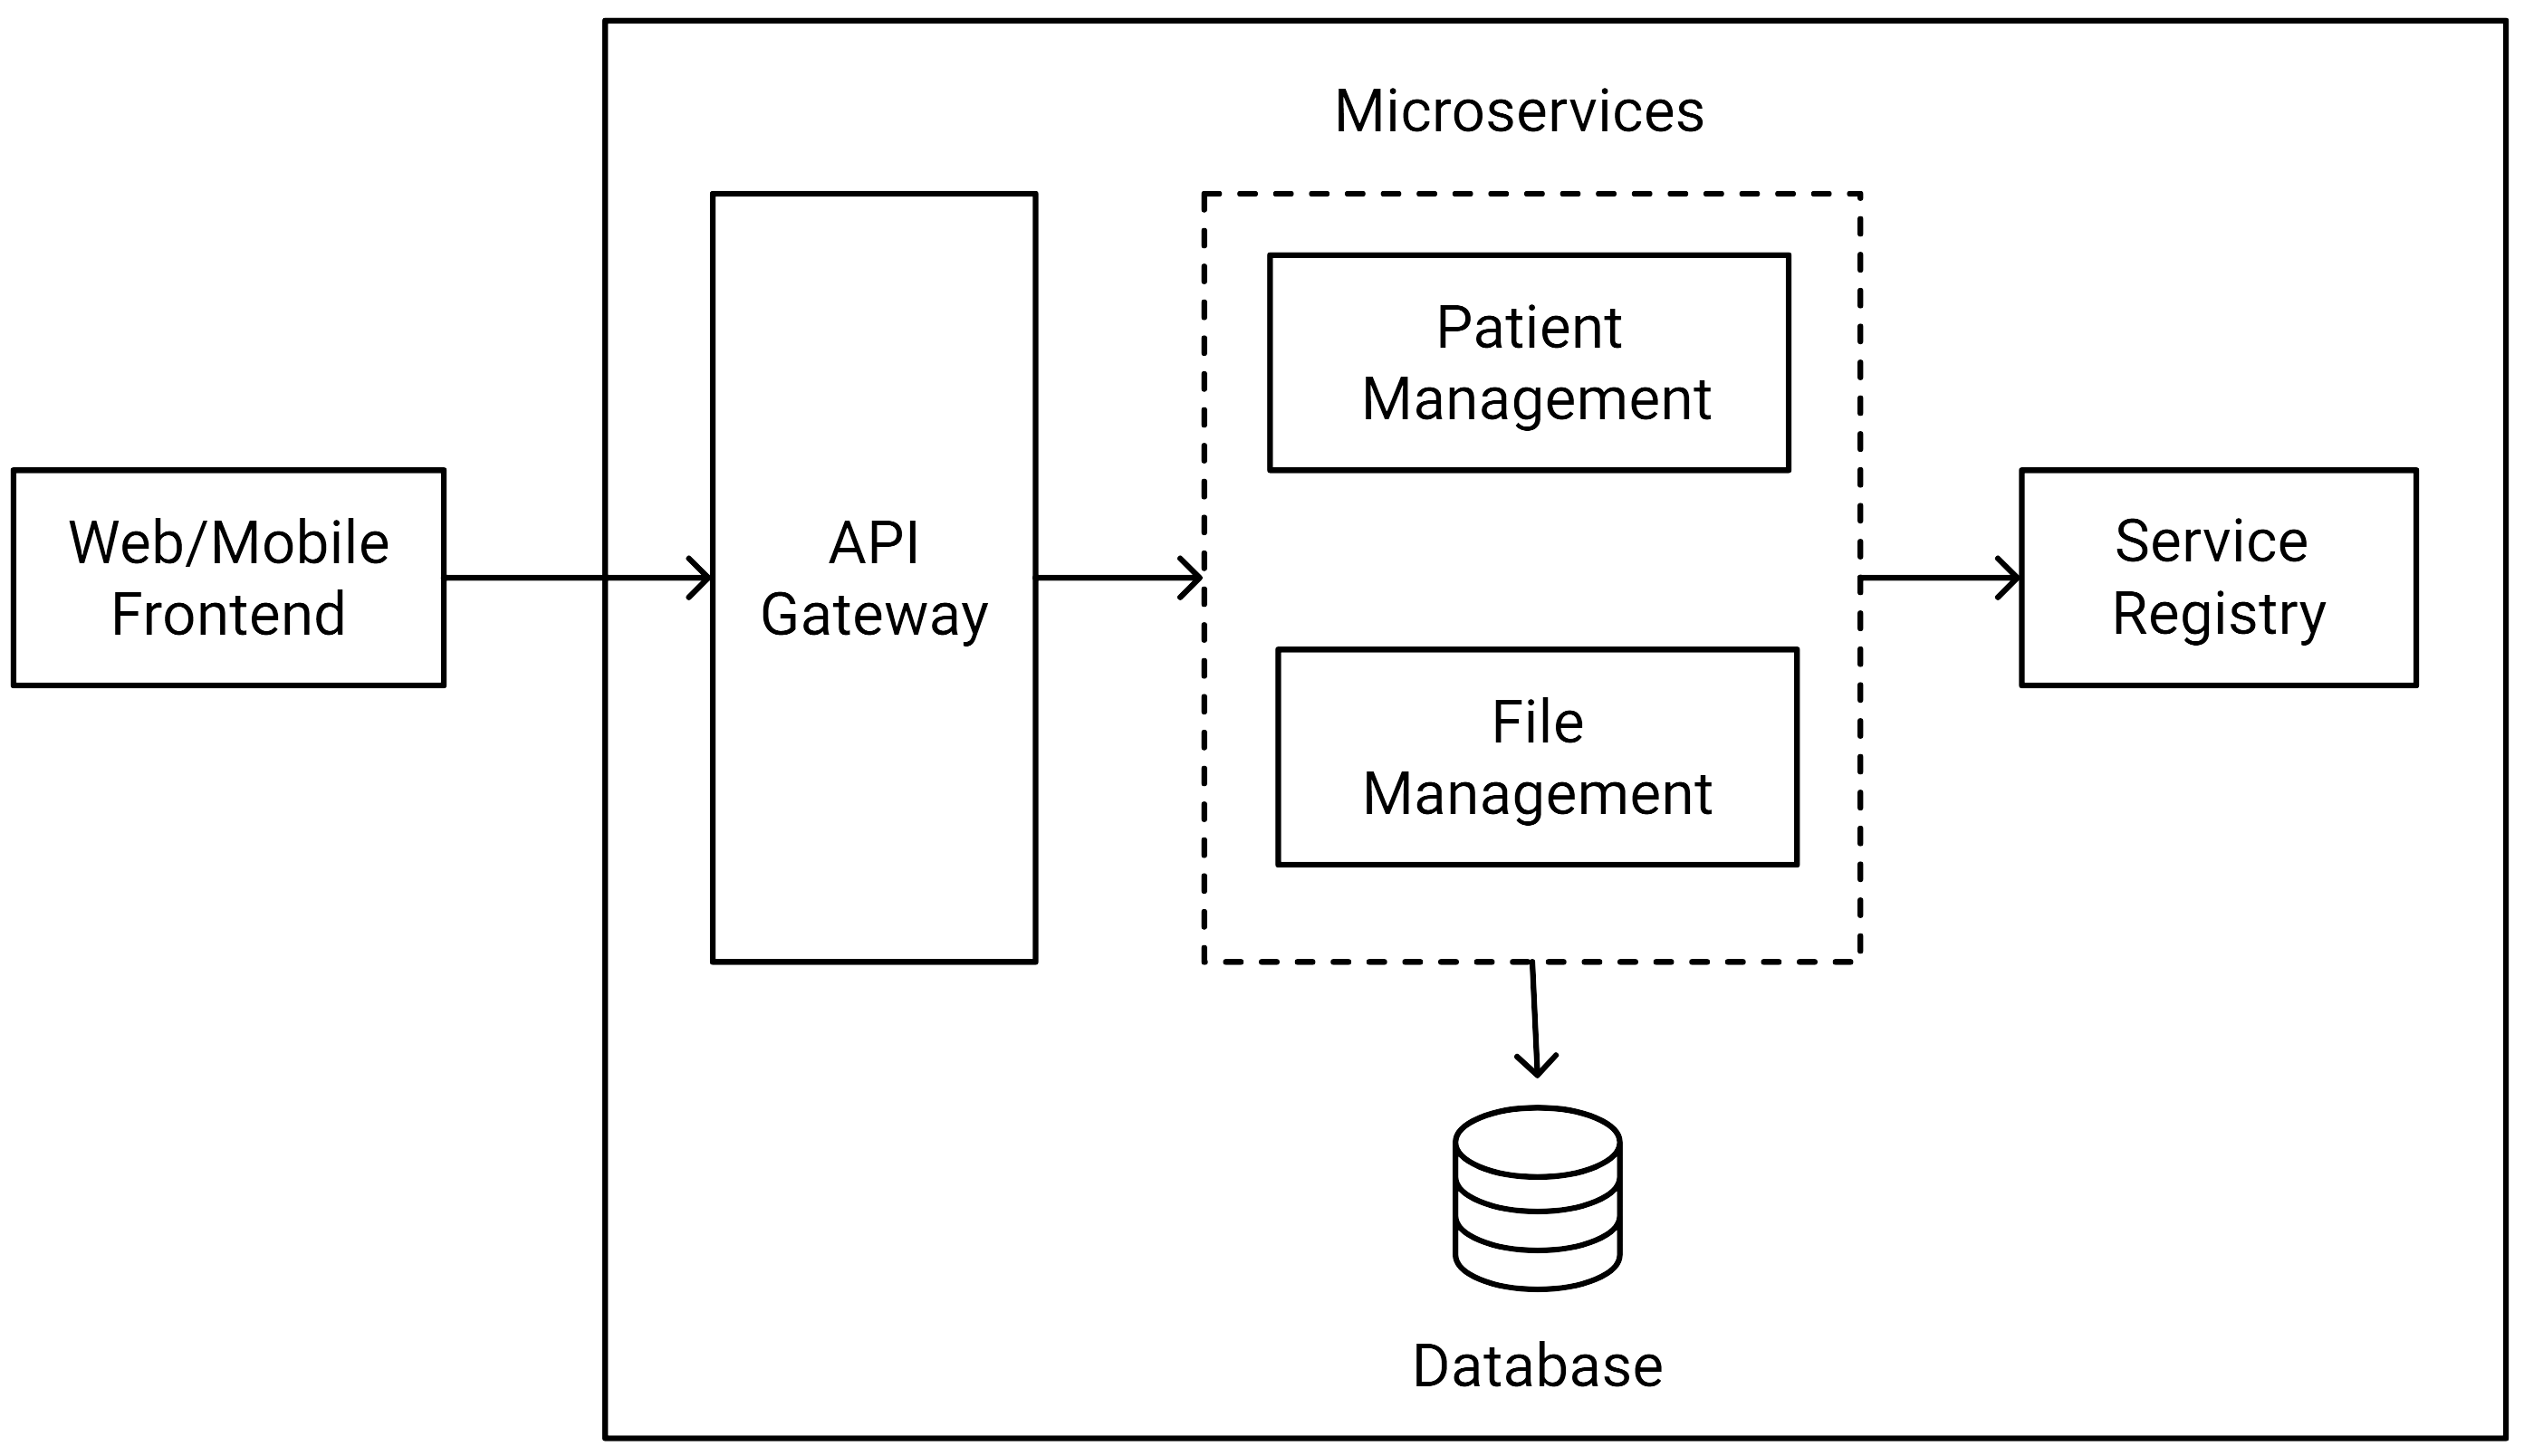
\includegraphics[width=0.95\linewidth]{images/EA/microservice-architecture.png}
        \caption{Microservice Architektur - CGM MAXX LITE}
        \label{fig:cgm-maxx-lite-microservices-architecture}
    \end{figure}

    Abbildung \ref{fig:cgm-maxx-lite-microservices-architecture} zeigt den Aufbau von CGM MAXX LITE mithilfe von Spring Boot. \\
    Die Software besteht aus folgenden Komponenten:
    \begin{itemize}
        \item \textbf{Web/Mobile Frontend}
        \begin{itemize}[label=$\circ$]
            \item Schnittstelle für Benutzerinteraktionen
            \item Kommuniziert mit der API, um Daten zu empfangen und zu senden
        \end{itemize}
        
        \item \textbf{API-Gateway}
        \begin{itemize}[label=$\circ$]
            \item Leitet eingehende Requests an die zuständigen Microservices weiter
        \end{itemize}
        
        \item \textbf{Microservices}
        \begin{itemize}[label=$\circ$]
            \item Patient Management \& File Management
        \end{itemize}

        \item \textbf{PostgreSQL-Datenbank}
        \begin{itemize}[label=$\circ$]
            \item Speichert alle Patientendaten sowie zugehörige Dateien
        \end{itemize}
        
        \item \textbf{Netflix Eureka Service Registry}
        \begin{itemize}[label=$\circ$]
            \item Registriert alle zum System gehörigen Microservices
            \item Ermöglicht die Kommunikation zwischen diesen
        \end{itemize}
    \end{itemize}

    In der Theorie wird für jedes Microservice eine eigene Datenbank erstellt, um eine höhere Ausfallsicherheit zu gewährleisten. 
    Aufgrund begrenzter Ressourcen, insbesondere in Bezug auf die Hardwareleistung und den zeitlich begrenzten Projektrahmen, wird eine zentrale Datenbank verwendet.

    Nun folgt eine genauere Beschreibung des Backends. Nicht nur die Microservices, sondern auch das API-Gateway
    müssen vom Service Registry registriert werden. Dies ist notwendig, um die vom Frontend kommenden Anfragen korrekt weiterzuleiten und die Kommunikation zwischen den Microservices zu ermöglichen. \lil{lst:service-registry-config} zeigt die Konfigurationsdatei der Service Registry Anwendung. \\
    
    \lstinputlisting[
        caption=\texttt{application.properties} - Service Registry,
        label=lst:service-registry-config,
    ]{sources/EA/application.properties}

    Grundsätzlich läuft die Service Registry auf dem Port 8761. Wird dieser Port freigegeben, kann über den Browser ein Dashboard aufgerufen werden, das alle registrierten Services auflistet. Zudem ist sie so konfiguriert, dass sie sich nicht selbst registriert. Bei den Microservices müssen die Werte \textbf{register-with-eureka} und \textbf{fetch-registry} auf \textbf{true} gesetzt werden. \lil{lst:file-service-config} zeigt einen Ausschnitt der Konfiguration des File Service: \\

    \lstinputlisting[
        caption=\texttt{application-docker.properties},
        label=lst:file-service-config,
    ]{sources/EA/application-docker.properties}

    Zusätzlich wird definiert, über welche URL die Service Registry erreicht werden kann. Da der File Service vor dem Hochladen einer Datei überprüfen muss, ob ein Patient mit der angegebenen ID existiert, benötigt dieser Zugriff auf den Patient Service.
    In Zeile 10 wird die URL des Patient Services definiert. Diese muss mit der im API-Gateway festgelegten URL (siehe \lil{lst:api-gateway}) übereinstimmen.

    Grundsätzlich ist kein API-Gateway notwendig. Allerdings erleichtert eine zentrale Schnittstelle die Verwaltung, da nur ein einziger Port nach außen hin freigegeben werden muss. 

    Im Folgenden werden jeweils ein REST-Controller des Patient Services und des File Services gezeigt, um einen Überblick über die verschiedenen Endpunkte zu geben. \\

    \lstinputlisting[
        caption=\texttt{PatientController.java},
        label=lst:patient-controller,
        firstline=16
    ]{sources/EA/PatientController.java}

    \lstinputlisting[
        caption=\texttt{FileInfoController.java},
        label=lst:file-info-controller,
        firstline=13
    ]{sources/EA/FileInfoController.java}

    Damit soll gezeigt werden, dass die Endpunkte verschiedener Anwendungen, die auf unterschiedlichen Ports betrieben werden, mithilfe eines API-Gateways über eine einzige Schnittstelle erreicht werden können.

    \clearpage

    Eine kurze Zusammenfassung der wichtigsten Endpoints:
    \begin{itemize}
        \item \textbf{PatientController} (siehe \lil{lst:patient-controller}) - Patient Management (Port 8081)
        \begin{itemize}[label=$\circ$]
            \item findPatients
            \item findById
        \end{itemize}
        
        \item \textbf{FileInfoController} (siehe \lil{lst:file-info-controller}) - File Management (Port 8082)
        \begin{itemize}[label=$\circ$]
            \item findFileById
            \item findFilesByPatientIdAndType
        \end{itemize}
    \end{itemize}

    Wird nun das Frontend gestartet, so werden verschiedene HTTP-Requests an das API-Gateway gesendet. 
    Werden die Dev-Tools in einem beliebigen Browser geöffnet und der Netzwerk-Tab ausgewählt, so kann überprüft werden, ob die Requests an den richtigen Microservice weitergeleitet werden.

    Klickt ein Arzt oder eine Ärztin auf eine bestimmte Person in der Patientenliste, so wird eine Detailansicht mit genaueren Informationen geöffnet. Dabei wird ein HTTP-Request an das Backend gesendet, um weitere Daten zu laden. 

    \begin{figure}[H]
        \centering
        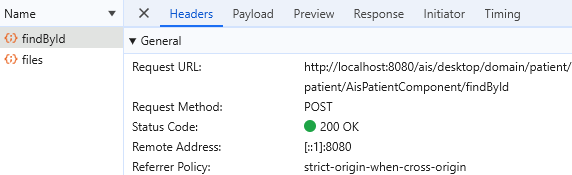
\includegraphics[width=1\linewidth]{images/EA/patient-management-http-request.png}
        \caption{HTTP-Request an den Patient Service}
        \label{fig:patient-management-http-request}
    \end{figure}

    Abbildung \ref{fig:patient-management-http-request} zeigt den HTTP-Request an den Patient Service, der korrekt über das API-Gateway und den Port 8080 weitergeleitet wird.

    Neben den Stammdaten werden auch Fotos und Audiodateien abgerufen, wobei der Request an den File Service weitergeleitet wird, wie in Abbildung \ref{fig:file-management-http-request} dargestellt.

    \begin{figure}[H]
        \centering
        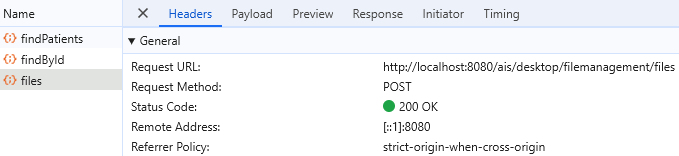
\includegraphics[width=1\linewidth]{images/EA/file-management-http-request.png}
        \caption{HTTP-Request an den File Service}
        \label{fig:file-management-http-request}
    \end{figure}

    Durch diese Architektur kann CGM MAXX LITE flexibel skaliert und durch die Entkopplung in mehrere Komponenten problemlos erweitert werden, was die Weiterentwicklung für die CGM Arztsysteme GmbH vereinfacht. 
    Im nächsten Kapitel wird das Thema Cloud Computing näher untersucht, um eine geeignete Lösung für den Betrieb der Software zu finden und die Unterschiede verschiedener Cloud-Modelle zu verdeutlichen. 
    

    \clearpage

    \section{Cloud Computing} \label{Cloud Computing}
    % --- C L O U D   C O M P U T I N G ---

Cloud Computing ist aus der heutigen Zeit nicht mehr wegzudenken. Täglich entstehen enorme Datenmengen, die gespeichert, verarbeitet und abgerufen werden müssen. Immer mehr Menschen und Unternehmen nutzen die Vorteile des Internets, um unabhängig von Standort und Uhrzeit auf bestimmte Dienste zuzugreifen. Von einfachen Ablagen in der Cloud bis hin zu Social-Media-Plattformen wie Instagram und Facebook wird alles mithilfe von Cloud Computing umgesetzt.

Besonders für Unternehmen ergeben sich dadurch völlig neue Möglichkeiten. Insbesondere die Software-Auslieferung hat sich grundlegend verändert. 
Software-Releases müssen nicht mehr Monate im Voraus geplant werden, sondern können dank neuer Technologien innerhalb weniger Minuten oder sogar Sekunden erfolgen.\\
\cite{EA:Web59}

All dies wäre ohne die Cloud undenkbar. Im Folgenden soll der Begriff Cloud Computing näher beschrieben werden.


    % --- D E F I N I T I O N ---

    \subsection{Definition}

    Die Cloud besteht aus einem großen Netzwerk von Servern, die auf der ganzen Welt verteilt sind und miteinander kommunizieren.
    Dabei ist es möglich, IT-Ressourcen, die in einem Rechenzentrum betrieben werden, zu mieten (siehe Abbildung \ref{fig:cloud-computing}). 
    
    Beispiele für solche Ressourcen sind:
    \begin{itemize}
        \item Server
        \item Speicher
        \item Datenbanken
    \end{itemize}

    Dies bietet den Vorteil, dass kein Geld für die Anschaffung von Hardware investiert werden muss. Bei Cloud Computing gibt es keine allgemein festgelegte Architektur. Es gibt mehrere Cloud-Modelle, die genutzt werden können, um die Wünsche der Kund/innen zu erfüllen.
    Diese werden in Abschnitt \ref{Cloud-Modelle} näher erläutert.
    \cite{EA:Web55}
    
    \begin{figure}[H]
        \centering
        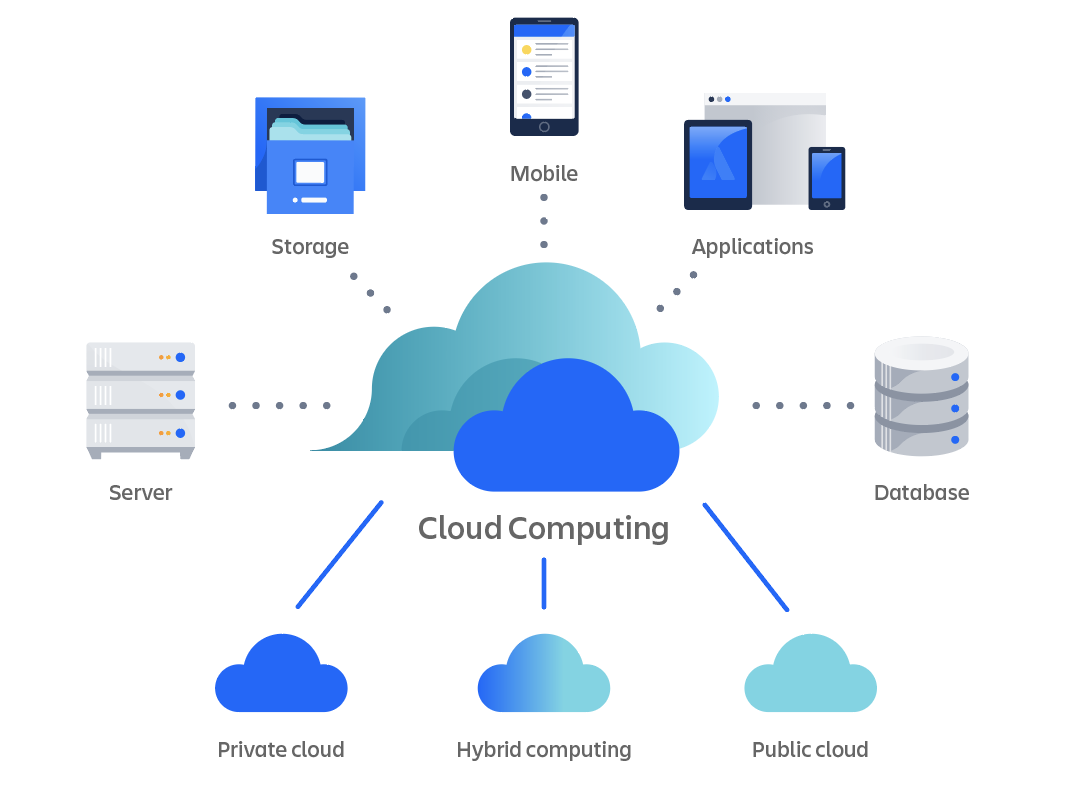
\includegraphics[width=0.75\linewidth]{images/EA/cloud-computing.png}
        \caption{Cloud Computing \\ \cite{EA:Web55}}
        \label{fig:cloud-computing}
    \end{figure}


    % --- C L O U D   -   M O D E L L E ---
    
    \subsection{Cloud-Modelle} \label{Cloud-Modelle}

        Grundsätzlich kann zwischen drei verschiedenen Arten von Cloud-Computing unterschieden werden:
        \begin{itemize}
            \item Public Cloud
            \item Private Cloud
            \item Hybrid Cloud
        \end{itemize}

    
        % --- P U B L I C   C L O U D ---
    
        \subsubsection{Public Cloud}
    
        Bei diesem Cloud-Computing-Modell sind die gesamten Ressourcen im Besitz des Cloud-Serviceanbieters. 
        Diese Cloud-Dienste können je nach Anbieter kostenlos oder kostenpflichtig sein und sind über das Internet erreichbar.
        Außerdem können die Ressourcen so ausgewählt werden, dass sie auf unterschiedliche Anwendungsfälle zugeschnitten werden können. Der/die Nutzer/in 
        wählt dabei einfach die benötigten Ressourcen über eine Benutzeroberfläche aus und kann somit innerhalb kürzester Zeit Software ausliefern. Alle zusätzlichen Aufgaben, wie die Bereitstellung und Verwaltung, werden vom Cloud-Anbieter übernommen. Der Einsatz spezieller Werkzeuge kann den Prozess der Systembereitstellung in der Cloud beschleunigen. Einige dieser Werkzeuge werden in Abschnitt \ref{IaC} näher beschrieben.
        \cite{EA:Web53, EA:Web54}
    
        Zu den bekanntesten Anbietern gehören:
        \begin{itemize}
            \item Amazon Web Services (AWS)
            \item Google Cloud
            \item Microsoft Azure
        \end{itemize}
    
        % --- P U B L I C   C L O U D   -   P R O S   &   C O N S ---
    
        \textbf{Vor- und Nachteile der Public Cloud}
    
        Zudem gibt es weitere Vorteile, die durch die Verwendung einer Public Cloud geschaffen werden können.
        Beispielsweise können die \textbf{Infrastrukturkosten gesenkt} werden, da keine Betriebskosten für einen lokal installierten Server mehr anfallen. Stattdessen wird nur noch für die tatsächlich genutzten Ressourcen in der Cloud bezahlt. Durch die flexible Verwaltung von Ressourcen ist auch die \textbf{Skalierung} unproblematisch. 
    
        Allerdings hat auch die Public Cloud ihre Schattenseiten, die berücksichtigt werden müssen. Speziell dann, wenn es um den Umgang mit sensiblen Daten geht, ist besondere Vorsicht geboten, da eine \textbf{unzureichende Konfiguration} zu \textbf{Sicherheitslücken} führen kann.
        Darüber hinaus muss sichergestellt werden, dass \textbf{stets eine stabile Internetverbindung besteht}, damit die in der Cloud bereitgestellten Dienste auch jederzeit erreicht werden können. \cite{EA:Web53} \\

        % --- E I N S A T Z G E B I E T E   -   P U B L I C   C L O U D ---
    
        \textbf{Einsatzgebiete der Public Cloud}
    
        Durch die zahlreichen Möglichkeiten, die Public Clouds bieten, können diese für extrem unterschiedliche Anwendungsfälle eingesetzt werden.
        Allgemein gesagt, eignet sich die Public Cloud besonders für Softwarelösungen, bei denen die genaue Auslastung vorab schwer abgeschätzt werden kann und/oder sich die Anforderungen im Laufe des Projekts häufig verändern.
        \cite{EA:Web53}

        \clearpage
        
    
        % --- P R I V A T E   C L O U D ---
    
        \subsubsection{Private Cloud}
    
        Da die Public Cloud trotz ihrer zahlreichen Vorteile nicht für jeden Anwendungsfall geeignet ist, gibt es weitere Arten von Cloud Computing, die in Betracht gezogen werden können. Eine davon ist die \textbf{Private Cloud}. 
    
        Der wesentliche Unterschied zur Public Cloud ist, dass die \textbf{Cloud-Computing-Ressourcen nicht mit anderen Personen geteilt} werden, sondern ausschließlich für Personen mit entsprechenden Zugriffsrechten zugänglich sind.
        
        Dies wird in Abbildung \ref{fig:private-cloud-vs-public-cloud} veranschaulicht:
        \begin{figure}[H]
            \centering
            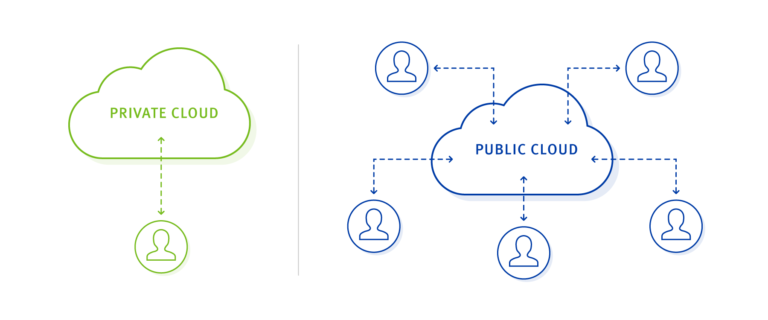
\includegraphics[width=0.85\linewidth]{images/EA/private-cloud-vs-public-cloud.png}
            \caption{Private Cloud vs. Public Cloud \\ \cite{EA:Img01}}
            \label{fig:private-cloud-vs-public-cloud}
        \end{figure}
    
        Zudem kann die Private Cloud weiter spezifiziert werden:
        \begin{itemize}
            \item \textbf{Lokale Private Cloud}
            \begin{itemize}[label=$\circ$]
                \item IT-Infrastruktur befindet sich am Standort des Kunden
                \item Bereitstellung \& Verwaltung erfolgt intern
            \end{itemize}
            \item \textbf{Cloud-Dienstanbieter}
            \begin{itemize}[label=$\circ$]
                \item Rechenressourcen werden in einem externen Rechenzentrum betrieben
                \item Ein Drittanbieter übernimmt die Bereitstellung und Verwaltung
            \end{itemize}
        \end{itemize}
    
        Verfügt ein Unternehmen über qualifiziertes Personal, das sich um die lokal installierte IT-Infrastruktur kümmert, kann auf externe Anbieter
        verzichtet werden. Ist dieses Kriterium nicht gegeben, so ist es wirtschaftlich sinnvoller, diese Aufgaben an einen Cloud-Dienstanbieter auszulagern, um die Anforderungen der Kundschaft effizient zu erfüllen.
        \cite{EA:Web54} \\
    
        % --- P R I V A T E   C L O U D   -   P R O S   &   C O N S ---
    
        \textbf{Vor- und Nachteile der Private Cloud}
    
        Dadurch, dass die Private Cloud eine isolierte Umgebung ist, auf die fremde Personen und Unternehmen keinen Zugriff haben, bietet diese Art von Cloud Computing einige Vorteile in Bezug auf \textbf{Sicherheit und Kontrolle}.
        Die Ressourcen können so angepasst werden, dass sie den Anforderungen der Auftraggebenden entsprechen.
    
        Wie die Public Cloud hat auch die Private Cloud ihre Nachteile. Um die möglichen Probleme der Private Cloud aufzuzeigen, wirft man einen Blick auf das Projekt CGM MAXX LITE. Wie in Abschnitt \ref{Projektbezug - Anforderungsanalyse} beschrieben, handelt es sich bei diesem Projekt um die Entwicklung einer Arztsoftware. Da diese Anwendung mit sehr sensiblen Daten arbeitet, die aus datenschutzrechtlichen Gründen nicht von unbefugten Personen eingesehen werden dürfen, ist die Private Cloud eine gute Lösung. 
    
        Sollte ein Arzt die Software erwerben und On-Premise\footnote{Software vor Ort betreiben} betreiben wollen, dann muss dafür eine \textbf{entsprechende Infrastruktur angeschafft und konfiguriert} werden, was erstens sehr \textbf{kostspielig} sein kann und \textbf{zusätzlichen Wartungsaufwand} erfordert. Zudem ist die Infrastruktur weniger flexibel als bei einem Drittanbieter, was im schlimmsten Fall zu Engpässen führen kann.
        \cite{EA:Web56} \\
    
    
        \textbf{Einsatzgebiete der Private Cloud}
    
        Wie aus dem obigen Absatz hervorgeht, eignet sich der Einsatz einer privat betriebenen Cloud besonders dann, wenn in etwa abgeschätzt werden kann, wie viele Ressourcen benötigt werden, um die Hardware gezielt auszuwählen und einen reibungslosen Betrieb des Softwaresystems zu gewährleisten. Auch für Anwendungen, bei denen ein hohes Maß an Sicherheit erforderlich ist, eignet sich dieses Cloud-Computing-Modell hervorragend.
    
        Weitere Beispiele wären Anwendungen in folgenden Bereichen:
        \begin{itemize}
            \item Finanzen
            \item Recht
            \item Politik
        \end{itemize}
    
        \cite{EA:Web56}
        
        \clearpage
    
    
        % --- H Y B R I D   C L O U D ---
    
        \subsubsection{Hybrid Cloud}
    
        Die letzte Art des Cloud Computings, die in dieser Arbeit beschrieben wird, ist die \textbf{Hybrid Cloud}. 
        Im Vergleich zu den zuvor erläuterten Cloud-Modellen kommen hier mehrere unterschiedliche Clouds zum Einsatz. 
        Es handelt sich also um eine \glqq{Mischform}\grqq\ bestehend aus Public und Private Cloud (siehe Abbildung \ref{fig:hybrid-cloud}).
    
        Die Clouds werden dabei so miteinander verbunden, dass Daten ausgetauscht werden können. Werden mehrere Clouds derselben Art (z.B. zwei öffentliche Clouds) eingesetzt, so spricht man von einer \textbf{Multi Cloud}.
    
        \begin{figure}[H]
            \centering
            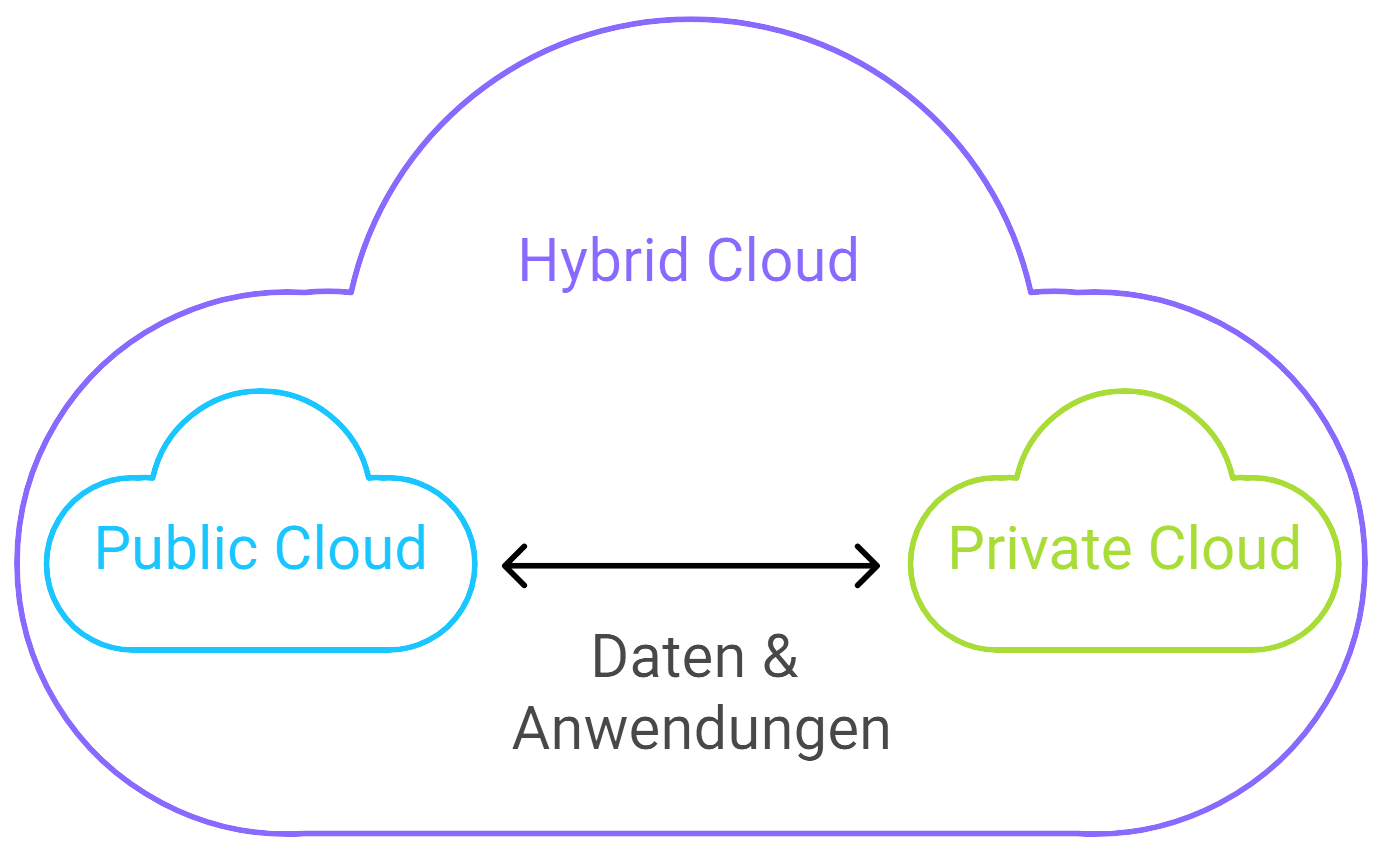
\includegraphics[width=0.6\linewidth]{images/EA/hybrid-cloud.png}
            \caption{Hybrid Cloud}
            \label{fig:hybrid-cloud}
        \end{figure}
    
        Speziell bei Anwendungen, bei denen ein großer Wert auf Datenschutz gelegt wird und worauf viele verschiedene Personen zugreifen können, ist es wichtig, die Daten sicher zu verwalten. In solchen Fällen ist es meist nicht mehr ausreichend, auf ein einziges Cloud-Modell zu vertrauen, weswegen immer häufiger auf hybride Cloud-Lösungen gesetzt wird.
         \cite{EA:Web57} 
    
         Um auf das zuvor genannte Beispiel zurückzukommen, das erklärt, wofür sich eine private Cloud besonders eignet, folgt nun eine kurze Ergänzung in Bezug auf die hybride Cloud:
    
        Arbeitet eine Applikation mit sensiblen Daten, so ist es sinnvoll, diese lokal oder in einer privat verwalteten Cloud abzulegen, während öffentlich zugängliche Dienste in der Public Cloud bereitgestellt werden sollten, um einen schnellen und einfachen Zugriff zu gewährleisten. 
    
        \clearpage
    
        \textbf{Vor- und Nachteile der Hybrid Cloud}
    
        Eine gezielte Kombination verschiedener Cloud-Umgebungen ermöglicht eine effizientere Ressourcennutzung, steigert die Flexibilität und kann Sicherheitsanforderungen besser erfüllen. Je nachdem, was betrieben werden soll, eignet sich eine Lösung besser als die andere. 
    
        Trotz der Vorteile beider Cloud-Modelle bringt die Hybrid Cloud auch neue Herausforderungen mit sich.
        Ein Nachteil ist beispielsweise ein erhöhter Aufwand in Bezug auf Verwaltung und Konfiguration. Grund dafür sind die vielen beteiligten Komponenten, die miteinander interagieren und im Auge behalten werden müssen. \cite{EA:Web58}
    

    \clearpage
    
    \section{Architekturentwurf} \label{Architekturentwurf}
    % --- A R C H I T E K T U R M O D E L L I E R U N G ---

Wie in Unterkapitel \ref{Allgemeines} bereits ausführlich beschrieben wurde, zählt die effiziente Umsetzung funktionaler und nicht-funktionaler Anforderungen des Auftraggebers zu den wichtigsten Zielen der Softwarearchitektur. Diese Anforderungen werden in Unterkapitel \ref{Anforderungsanalyse} näher erläutert. Basierend auf den Ergebnissen der Anforderungsanalyse wird ein Architekturstil ausgewählt, wobei eine Auswahl moderner Architekturstile in Unterkapitel \ref{Architekturstile} näher beschrieben wird. Darüber hinaus sind weitere Entscheidungen zu treffen, wie die Wahl der Technologien, die Unterteilung des Systems in kleinere, verwaltbare Teile und andere relevante Aspekte.

Dieser Prozess wird in regelmäßigen Abständen wiederholt, um anhand von Feedback und neuen Erkenntnissen, die während der Entwicklung gewonnen werden, Anpassungen vorzunehmen und die Architektur der Software kontinuierlich zu verbessern.

Bevor mit der Implementierung der Software begonnen wird, ist es essenziell, dass ein erster Entwurf der Architektur vorliegt.
Eine gute Planung bietet den Projektteammitglieder nicht nur eine klare Orientierungshilfe, sondern hilft auch, potenzielle Herausforderungen frühzeitig zu erkennen.
\cite{EA:Web15, EA:Web16}


% --- A R C H I T E K T U R M O D E L L I E R U N G ---

\subsection{Architekturmodellierung} \label{Architekturmodellierung}

    Wie in Abschnitt \ref{Die Rolle von Softwarearchitekt/innen} beschrieben, muss der/die Softwarearchitekt/in in der Lage sein, das Projektteam in eine bestimmte Richtung zu lenken. Dabei ist es wichtig, dass alle Teammitglieder sowohl die funktionalen als auch die nicht-funktionalen Anforderungen des Projekts kennen und zumindest einen groben Überblick über die zugrundeliegende Softwarearchitektur haben.

    Da die Architektur eines Softwaresystems sehr komplex und umfangreich sein kann, können \textbf{Visualisierungstechniken} eingesetzt werden, um die \textbf{Komplexität zu reduzieren}. Dies bezeichnet man als Architekturmodellierung, bei der die wesentlichen Eigenschaften des Systems identifiziert und dargestellt werden, um das System besser zu verstehen. 
    
    Das Ziel ist es, einen klaren Überblick zu schaffen und fundierte Entscheidungen anhand dieser Darstellungen zu treffen.
    Nicht nur das Projektteam profitiert davon, sondern auch neue Teammitglieder, die so schneller ins Projekt integriert werden können.

    Es gibt zahlreiche Tools und Standards, die für die Visualisierung der Softwarearchitektur verwendet werden können.
    Im Folgenden werden zwei der bekanntesten Modellierungstechniken näher beschrieben.
    \cite{EA:Web12, EA:Web13, EA:Web14}


     % --- U N I F I E D   M O D E L I N G   L A N G U A G E   ( U M L ) ---

    \subsubsection{Unified Modeling Language (UML)} \label{UML}

    Die Unified Modeling Language (UML) ist eine standardisierte Modellierungssprache, die verwendet wird, um bestimmte Teile eines Softwaresystems grafisch darzustellen.

    Durch den Einsatz von UML können Diagramme erstellt werden, die als Kommunikationsmittel zwischen unterschiedlichen Stakeholdern genutzt werden können. \\
    Diese Diagramme bieten den Vorteil, dass sie auch von Personen verstanden werden können, die keine Programmierkenntnisse besitzen und komplexe Systeme einfach darstellen.
    \cite{EA:Web18, EA:Web19}

    Es gibt 14 offiziell anerkannte Arten von UML-Diagrammen, die in \textbf{zwei Kategorien} unterteilt werden:
    \begin{itemize}
        \item Strukturelle Diagramme
        \item Verhaltensdiagramme
    \end{itemize}

    In Abbildung \ref{fig:uml-diagrams} sind die verschiedenen UML-Diagrammtypen dargestellt:

    \begin{figure}[H]
        \centering
        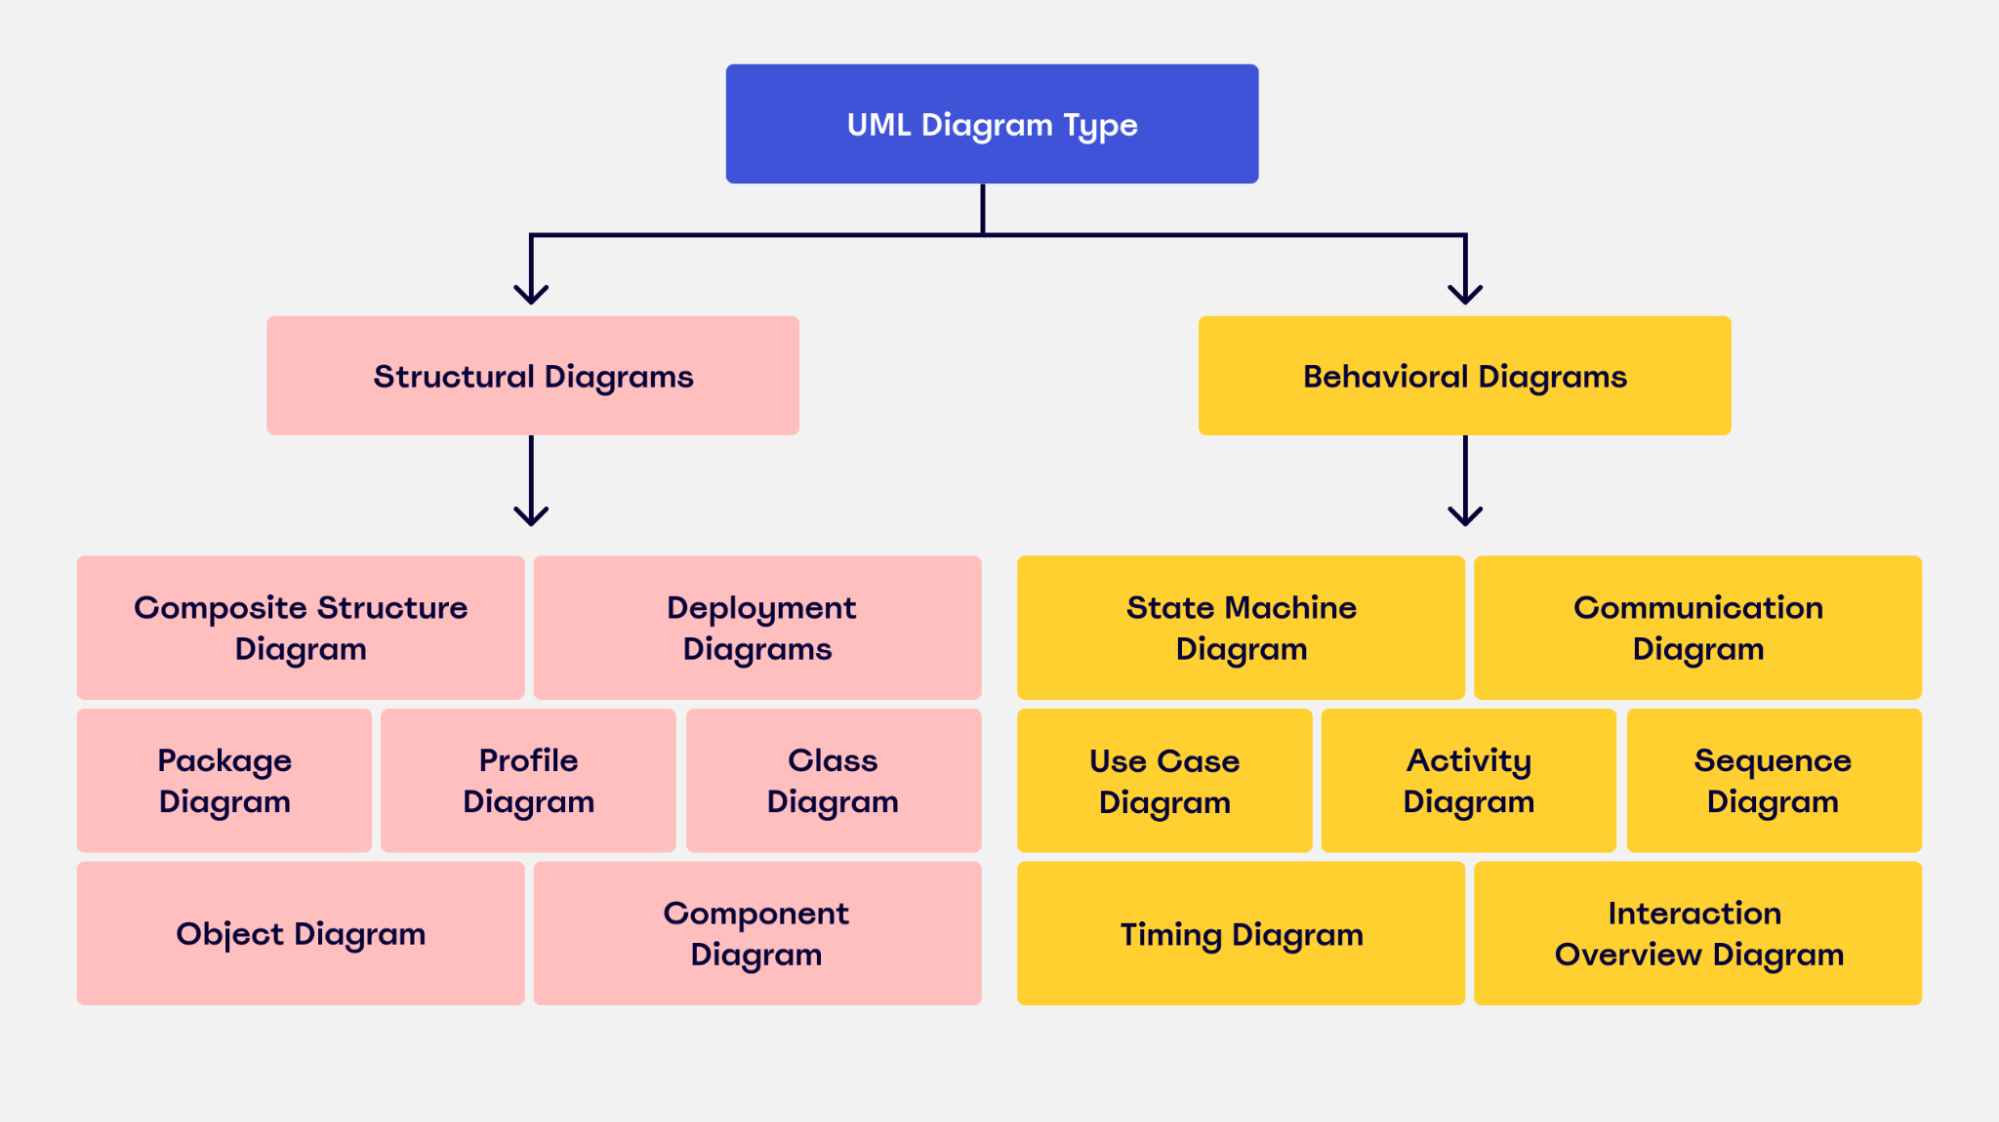
\includegraphics[width=1\linewidth]{images//EA/uml-diagrams.png}
        \caption{Arten von UML-Diagrammen \\ \cite{EA:Web17}}
        \label{fig:uml-diagrams}
    \end{figure}

    \clearpage

    Da es den Rahmen dieser Arbeit sprengen würde, jeden einzelnen UML-Diagrammtyp im Detail zu erklären, wird die allgemeine Unterscheidung zwischen Struktur- und Verhaltensdiagrammen betrachtet. Anschließend wird jeweils ein Struktur- und ein Verhaltensdiagramm näher beschrieben, die in der Praxis besonders häufig Anwendung finden und in Bezug auf das Projekt \textbf{CGM MAXX LITE} von Bedeutung sind.


    % --- S T R U K T U R E L L E   D I A G R A M M E ---

    \textbf{Strukturelle Diagramme} veranschaulichen den \textbf{Aufbau eines Softwaresystems} oder einzelner Teile davon. 
    Dabei werden Komponenten wie Klassen, Objekte und Module sowie deren Beziehungen dargestellt, die für die Struktur der Software entscheidend sind.


        % --- K L A S S E N D I A G R A M M ---

        Das bekannteste Strukturdiagramm ist das \textbf{Klassendiagramm}, wobei das System, oder nur ein Teil davon, durch Klassen abgebildet wird.
        Jede Klasse hat dabei bestimmte Attribute (Daten) und Methoden (Funktionen), die für unterschiedliche Aufgaben genutzt werden können.
        \cite{EA:Web17, EA:Web18}
    
        Ein Beispiel für ein Klassendiagramm ist in Abbildung \ref{fig:class-diagram-file-upload} zu finden.
        Es zeigt die Klassen, die im Rahmen des Projekts CGM MAXX LITE für den File-Upload erforderlich sind.
    
        Hierbei handelt es sich um die \textbf{Klassen einer Spring-Boot-Applikation}. Da diese Anwendung neben dem Hochladen von Dateien auch noch weitere Funktionalitäten bietet, konzentriert sich dieses Diagramm \textbf{nur} auf die \textbf{Klassen, die für das Hochladen von Dateien relevant sind}. 
        Dadurch wird ein besserer Überblick gewährleistet und es ist einfacher das Diagramm zu verstehen, ohne sich von irrelevanten Klassen oder Methoden ablenken zu lassen.
    
        Hier eine kurze Erklärung der wichtigsten Klassen:
        \begin{itemize}
            \item \lstinline{FileUploadController} ... RESTful-Controller, der die Schnittstellen für die Kommunikation zwischen Frontend und Backend bereitstellt.
            
            \item \lstinline{FileUploadServiceImpl} ... Service, der die gesamte Business-Logik umfasst. Dazu gehört nicht nur das Speichern von Fotos und Audioaufnahmen, sondern auch die richtige Benennung dieser Dateien.
            
            \item \lstinline{FileInfoService} ... wird verwendet, um die Anzahl der Dateien zu ermitteln, die an einem bestimmten Tag für einen bestimmten Patienten hochgeladen wurden. Dies ist notwendig für eine einheitliche Benennung der Dateien.
            
            \item \lstinline{PatientService} ... überprüft, ob der/die Patient/in, für den eine Datei hochgeladen werden soll, existiert.
            
            \item \lstinline{FileRepository} ... verwaltet \lstinline{File}-Entitäten (CRUD\footnote{Abkürzung für Create, Read, Update und Delete}-Operationen)
        \end{itemize}
    
        \begin{figure}[H]
            \centering
            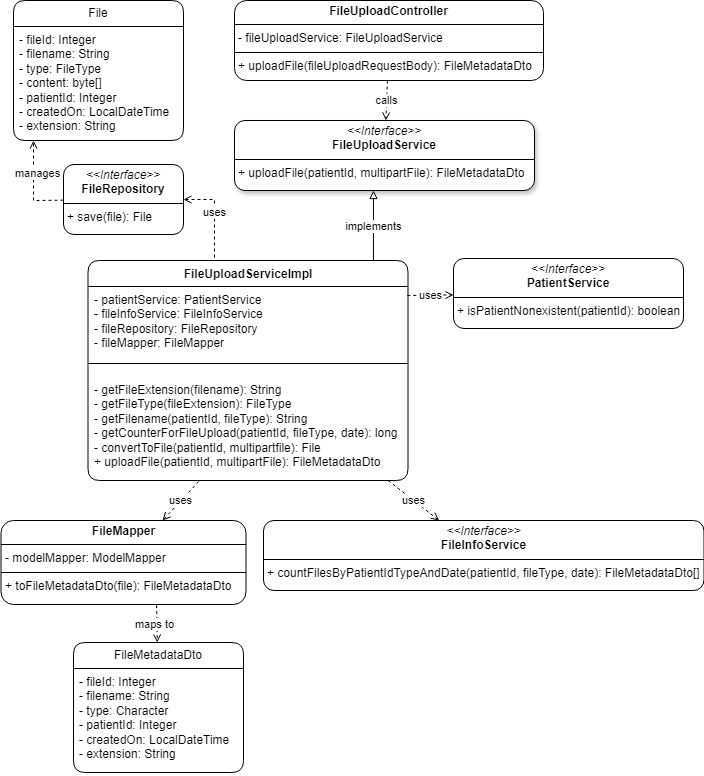
\includegraphics[width=1\linewidth]{images/EA/uml-class-diagram.png}
            \caption{Klassendiagramm - File Upload im Projekt CGM MAXX LITE}
            \label{fig:class-diagram-file-upload}
        \end{figure}

        Neben den Klassen in Abbildung \ref{fig:class-diagram-file-upload} sind auch die Beziehungen zwischen diesen durch unterschiedliche Pfeile gekennzeichnet, die durch das Hinzufügen von Beschriftungen noch leichter nachvollzogen werden können.

        \clearpage

        Im oben abgebildeten Klassendiagramm kommen nur zwei Arten von Beziehungen zum Einsatz:
        \begin{itemize}
            \item Vererbung (Inheritance)
            \item Abhängigkeit (Dependency)
        \end{itemize}

        Dabei implementiert \lstinline{FileUploadServiceImpl} das Interface \lstinline{FileUploadSerive}. Die restlichen Beziehungen zeigen Abhängigkeiten, bei denen bestimmte Klassen mithilfe von \textbf{Dependency Injection\footnote{Technik, bei der Objekte ihre Abhängigkeiten von anderen Objekten erhalten \cite{EA:Web22}}} eingebunden werden, um bestimmte Methoden aufzurufen. 
        \cite{EA:Web21}

        Auf den ersten Blick wirkt das Diagramm möglicherweise etwas komplex, betrachtet man es jedoch genauer, erkannt man, dass es \textbf{nach außen hin nur eine Schnittstelle} gibt, auf die zugegriffen werden kann. Im Folgenden wird gezeigt, wie auf die Schnittstelle zugegriffen werden kann. \\
    
       \lstinputlisting[
            caption=\texttt{FileUploadController.java},
            label=lst:file-upload,
            firstline=10
        ]{sources/EA/FileUploadController.java}
    
        Der in \lil{lst:file-upload} definierte REST-Controller ermöglicht das Hochladen einer Datei für eine/n Patient/in über einen \textbf{POST-Request}. Dabei wird der \\ \lstinline{FileUploadService} aufgerufen, um die Datei korrekt zu benennen und anschließend in der Datenbank zu speichern.

        \clearpage
    
        % --- V E R H A L T E N S D I A G R A M M E ---

        Neben strukturellen Diagrammen gibt es auch \textbf{Verhaltensdiagramme}.
        Diese stellen das dynamische Verhalten eines Systems dar.
        Dabei spielt nicht nur das Geschehen innerhalb des Systems eine Rolle, sondern auch wie das System mit anderen Systemen und Benutzern interagiert. Verhaltensdiagramme eignen sich deshalb besonders gut, um \textbf{Abläufe und Geschäftsprozesse} zu \textbf{visualisieren}.
        \cite{EA:Web18, EA:Web20}

        Um ein Diagramm zu erstellen, das nicht nur die Struktur der Klassen darstellt, sondern auch erklärt, in welcher Reihenfolge bestimmte Interaktionen erfolgen, kann ein sogenanntes \textbf{Sequenzdiagramm} verwendet werden. Dies ermöglicht es, den genauen Ablauf eines bestimmten Prozesses nachzuvollziehen.
        \cite{EA:Web23, EA:Web24} \\

        \begin{figure}[H]
            \centering
            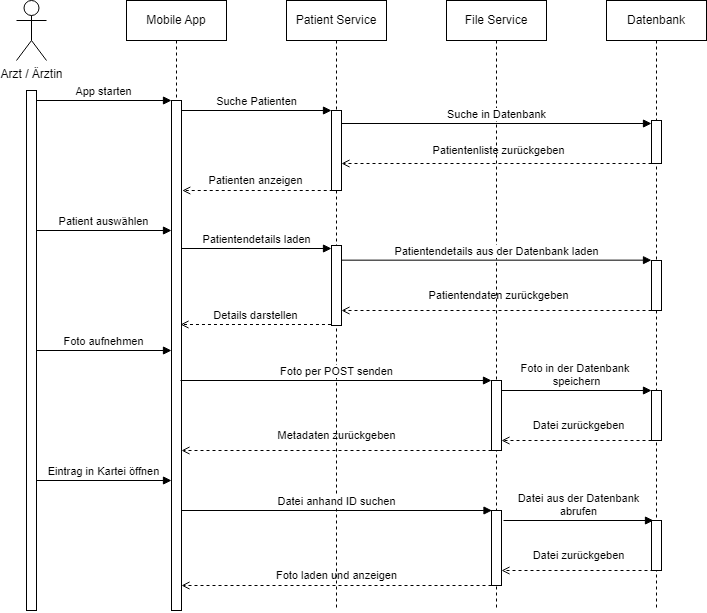
\includegraphics[width=1\linewidth]{images/EA/uml-sequence-diagram.png}
            \caption{Sequenzdiagramm - File Upload im Projekt CGM MAXX LITE}
            \label{fig:sequence-diagram-file-upload}
        \end{figure}

        \clearpage

        Um den Unterschied zwischen strukturellen Diagrammen und Verhaltensdiagrammen zu verdeutlichen, stellt das Sequenzdiagramm in Abbildung \ref{fig:sequence-diagram-file-upload} ebenfalls den File-Upload dar. Während das Klassendiagramm in Abbildung \ref{fig:class-diagram-file-upload} die Struktur der Klassen beschreibt und einen Bezug zum Code herstellt, zeigt das Sequenzdiagramm die notwendigen Schritte, um eine Datei in der Datenbank abzulegen und später in der App abzurufen.

        Folgende Elemente werden im Sequenzdiagramm \ref{fig:sequence-diagram-file-upload} verwendet:
        \begin{itemize}
            \item Akteur/innen
            \item Objekte
            \item Lebenslinien
            \item Aktivitätsbalken
            \item Synchrone Nachrichten (durchgezogene Linie mit ausgefüllter Spitze)
            \item Asynchrone Antworten (strichlierte Linie mit offener Spitze)
        \end{itemize}

        Im Folgenden wird der Ablauf des Sequenzdiagramms näher beschrieben, um den Einsatz und die Bedeutung der einzelnen Elemente zu erklären. \cite{EA:Web24}

        Da die Software CGM MAXX LITE hauptsächlich von \textbf{Ärzten/innen} verwendet wird, gibt es hier \textbf{nur einen Akteur/eine Akteurin}. Akteur/innen sind also Entitäten, die mit dem System interagieren. Die \textbf{Objekte} stellen \textbf{einzelne Teile des Systems} dar.
        Dieses besteht aus einer mobilen Benutzeroberfläche, einer zentralen Datenbank und zwei Microservices. Der eine Microservice ist verantwortlich für die Patientenverwaltung, das andere kümmert sich um die Verwaltung von Fotos und Audioaufnahmen. Die \textbf{strichlierten Linien unterhalb der Objekte} stellen deren \textbf{Lebenslinien} dar. Die \textbf{darüberliegenden Balken} bezeichnet man als \textbf{Aktivitätsbalken}. Diese stellen dar, wann auf bestimmte Objekte zugegriffen wird.
        Was genau passiert, wird durch \textbf{verschiedene Pfeile und kurze Beschreibungen} dargestellt.
        Die Akteur/innen können dabei nur auf die mobile Applikation zugreifen, die im Hintergrund auf die einzelnen Services zugreift. 

        Möchte ein Arzt oder eine Ärztin ein Foto hochladen, werden zunächst die Patient/innen aus der Datenbank geladen. Anschließend kann der/die gewünschte Patient/in ausgewählt werden. Dabei wird die Detailansicht geöffnet und es kann ein Foto aufgenommen werden. Ein POST-Request wird an den File Service gesendet, der das Foto verarbeitet, benennt es korrekt, in der Datenbank speichert und  anschließend die Metadaten der hochgeladenen Datei zurückgibt, um zu bestätigen, dass der Upload erfolgreich war.
        
        \clearpage
    

    % --- C 4 - M O D E L L ---

    \subsubsection{C4-Modell}

    Neben UML gibt es zahlreiche weitere Methoden, um die Architektur einer Software zu modellieren.
    Eine davon ist das \textbf{C4-Modell}, dessen Name für \textbf{Context, Containers, Components und Code} steht.
    Ähnlich wie UML zielt auch das C4-Modell darauf ab, das Verständnis unterschiedlicher Interessensgruppen zu verbessern, um eine Grundlage für erfolgreiche Projektergebnisse zu schaffen. Dabei wird das \textbf{System in vier Ebenen dargestellt}. 
    \cite{EA:Web25, EA:Web26, EA:Web28}

    Als nächstes werden die einzelnen Ebenen näher beschrieben:

    Die \textbf{erste Ebene} bezieht sich auf den \textbf{Systemkontext}. Bei einem Systemkontext-Diagramm liegt der Fokus darauf, 
    einen \textbf{groben Überblick über das System} zu schaffen, ohne näher auf spezifische Technologien und technische Details einzugehen.
    Genauer gesagt beschreibt es, wofür das System zuständig ist, von wem es verwendet wird und wie es mit anderen Systemen interagiert.
    Solche Diagramme eignen sich besonders gut, um mit nicht-technischen Stakeholdern zu kommunizieren.
    \cite{EA:Web27}

    In Abbildung \ref{fig:c4-system-context-diagram} wird das Systemkontext-Diagramm für das Projekt CGM MAXX LITE dargestellt:

    \begin{figure}[H]
        \centering
        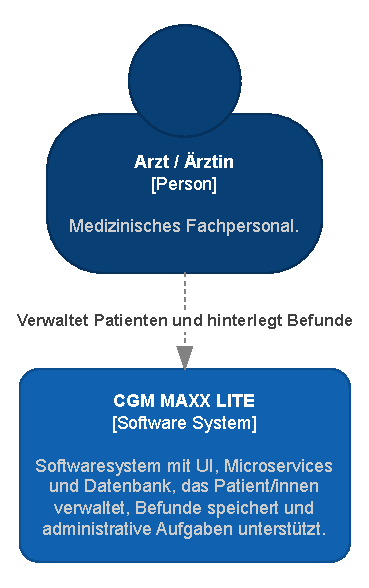
\includegraphics[scale=1.05]{pdf/EA/c4-system-context-diagram.pdf}
        \caption{Systemkontext-Diagramm - CGM MAXX LITE}
        \label{fig:c4-system-context-diagram}
    \end{figure}

    \clearpage

    Die \textbf{zweite Ebene} stellt die \textbf{einzelnen Container eines Systems} dar. Container stellen die grundlegenden Bestandteile eines Systems dar, die unabhängig voneinander gestartet, bereitgestellt und betrieben werden können.
    \textbf{Container-Diagramme} zeigen zusätzlich auch die verwendeten Technologien und wie die Container miteinander kommunizieren. 
    Sie können eingesetzt werden, um \textbf{Softwareentwickler/innen bei der Entwicklung zu unterstützen}. Das bietet den Vorteil, dass Abhängigkeiten zwischen Container einfacher nachvollzogen werden können. 
    \cite{EA:Web28}
    
    \begin{figure}[H]
        \centering
        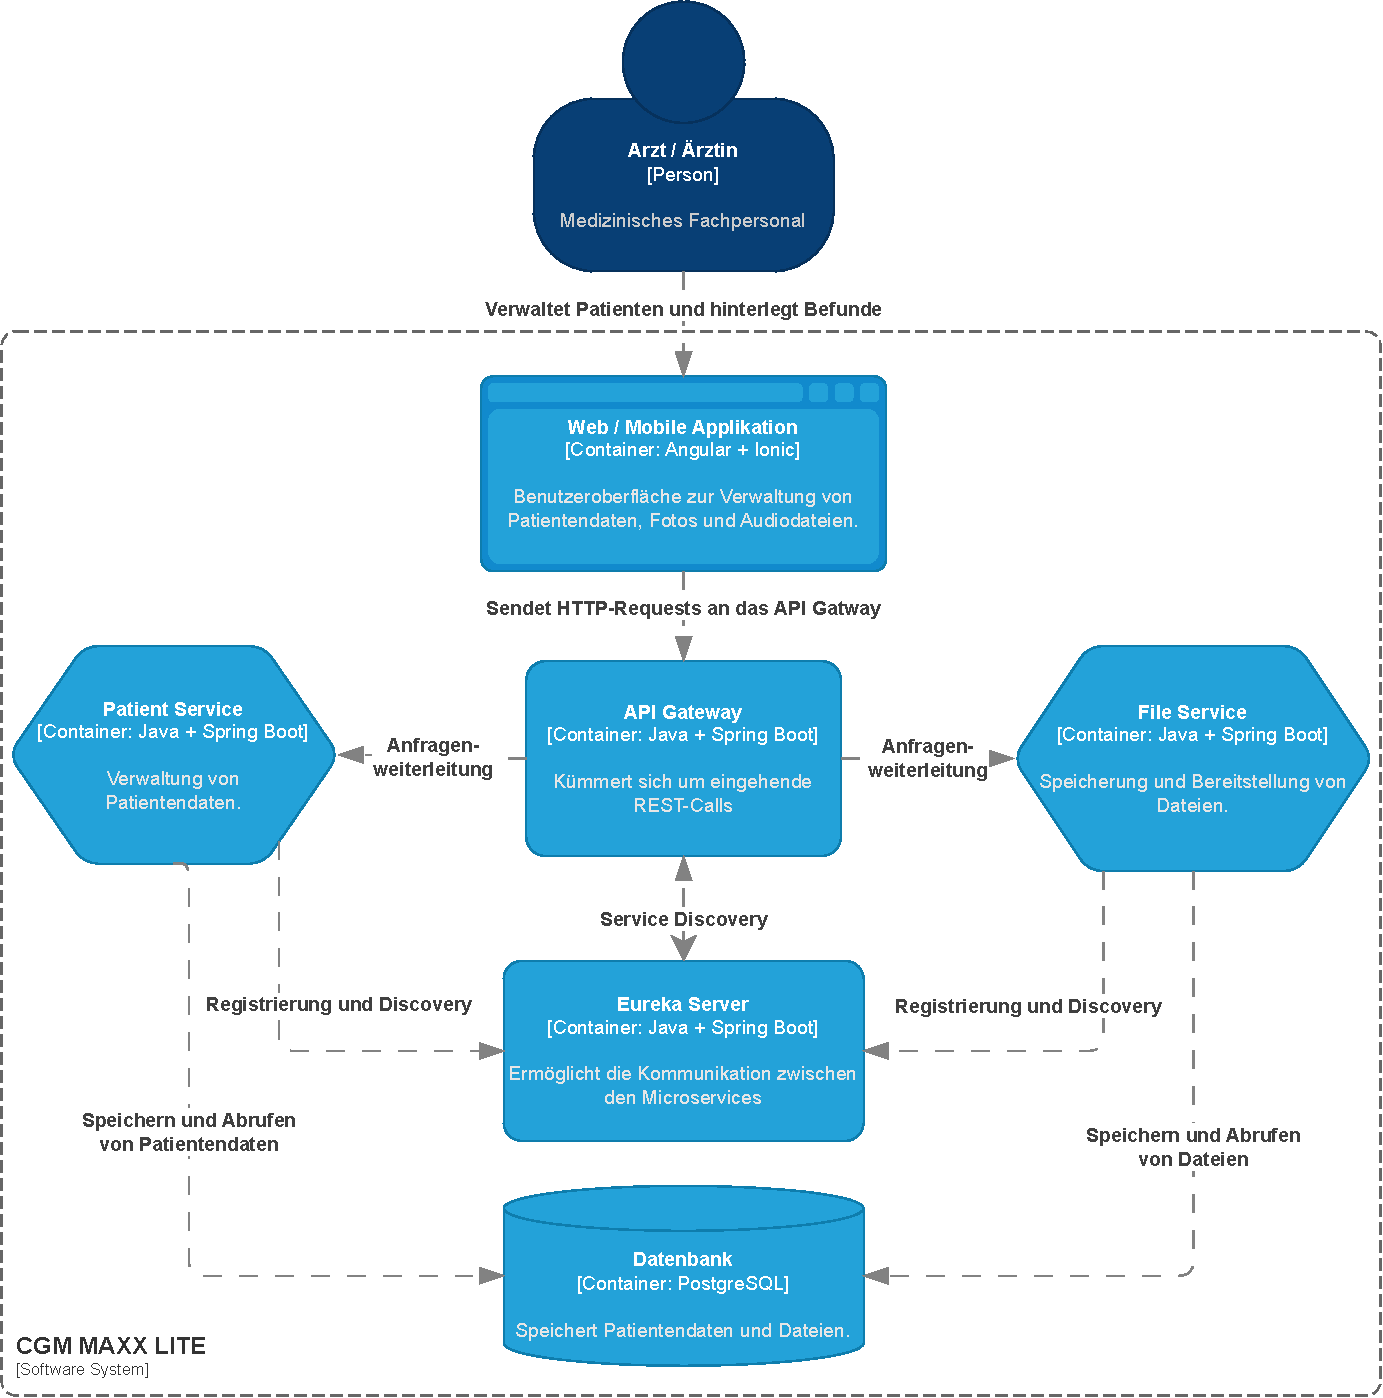
\includegraphics[scale=0.7]{pdf/EA/c4-container-diagram.pdf}
        \caption{Container-Diagramm - CGM MAXX LITE}
        \label{fig:c4-container-diagram}
    \end{figure}

    In Abbildung \ref{fig:c4-container-diagram} wird ein Container-Diagramm dargestellt, das die wichtigsten Bestandteile des Projekts CGM MAXX LITE zeigt. 
    
    Dabei gibt es unterschiedliche Arten von Containern:
    \begin{itemize}
        \item Web-App / Mobile App
        \item API-Gateway
        \item Microservices
        \item Service Discovery Server
        \item Datenbank
    \end{itemize}

    Eine genaue Beschreibung der einzelnen Container ist in Abschnitt \ref{Projektbezug - Architekturstil} zu finden.

    Da es zu umfangreich wäre, für jede Ebene des C4-Modells ein spezifisches Diagramm für CGM MAXX LITE zu erstellen, und es zudem schwierig ist, alle Komponenten auf einer Seite darzustellen, werden die folgenden Ebenen ausschließlich textlich beschrieben.

    Die \textbf{dritte Ebene} ermöglicht einen genaueren Blick auf die \textbf{Elemente innerhalb eines Containers}.
    Mithilfe eines \textbf{Komponentendiagramms} kann dargestellt werden, welche Aufgaben die einzelnen Komponenten erledigen, wie sie miteinander interagieren und welche Technologien oder Implementierungen dabei zum Einsatz kommen.
    \cite{EA:Web27, EA:Web28}

    Ein Beispiel für eine Komponente ist ein REST-Controller in Spring Boot. Bezieht man sich dabei auf das Projekt, so wäre die Java-Klasse \textbf{FileUploadController.java} in \lil{lst:file-upload} eine Komponente.

    Die \textbf{vierte} und letzte \textbf{Ebene} des C4-Modells betrachtet die Implementierung einzelner Komponenten.
    Dazu können \textbf{UML-Klassendiagramme} eingesetzt werden. Auch hierfür gibt es bereits ein Beispiel in Abbildung \ref{fig:class-diagram-file-upload}
    Solche Diagramme müssen oft nicht selbst erstellt werden, da sie mithilfe von IDEs\footnote{Integrierte Entwicklungsumgebung} automatisch erstellt werden können.
    \cite{EA:Web28}

    \clearpage

    \subsubsection{Überleitung}
    
    Bevor mit dem nächsten Thema fortgesetzt wird, hier eine kurze Zusammenfassung der wichtigsten Erkenntnisse:
    
    Es gibt unzählige verschiedene Möglichkeiten, um die Architektur einer Software grafisch darzustellen. 
    Diese Visualisierungen können als Kommunikationsmittel eingesetzt werden und helfen dabei, ein besseres Verständnis für das System zu schaffen, unabhängig davon, ob eine Person technische Fähigkeiten besitzt oder nicht. 
    Basierend auf der Zielgruppe können unterschiedliche Diagramme verwendet werden.    
    Je nach Anwendungszweck eigenen sich bestimmte Diagramme besser als andere.
    

% --- C L O U D - S P E Z I F I S C H E   A R C H I T E K T U R E N T S C H E I D U N G E N ---

\subsection{Cloud-spezifische Architekturentscheidungen}

Da der Entwurf einer Software weit mehr als nur die Modellierung betrifft, gibt es einige weitere Entscheidungen, die getroffen werden müssen.
Wie der Name dieser Arbeit bereits verrät, liegt der Fokus auf cloudbasierten Systemen. Neben Planung und Entwicklung muss die Software auch in der Cloud bereitgestellt werden, um sie für die Nutzer/innen zugänglich zu machen.

Damit Anwendungen sicher, zuverlässig und skalierbar in der Cloud bereitgestellt werden können, gibt es \textbf{Entwurfsmuster}, die eingesetzt werden, um bestimmte Probleme der Cloud zu umgehen. Um Software schneller bereitzustellen, kann die Infrastruktur mithilfe von \textbf{Infrastructure as Code} automatisch erstellt werden. \textbf{DevOps und Automatisierung} spielen ebenfalls eine bedeutende Rolle, um Anwendungen einfach bereitzustellen.
\cite{EA:Web30, EA:Web31}

Im weiteren Verlauf wird näher auf diese Themen eingegangen.


    % --- E N T W U R F S M U S T E R   F Ü R   D I E   C L O U D ---

    \subsubsection{Entwurfsmuster für die Cloud} \label{Entwurfsmuster für die Cloud}

    Wie zuvor erwähnt werden Entwurfsmuster eingesetzt, um \textbf{Software zuverlässig in der Cloud zu betreiben}. 
    Vor allem bei verteilten Systemen, bei denen mehrere Komponenten über das Netzwerk miteinander kommunizieren, kann es zu Schwierigkeiten kommen.
    Beispiele dafür sind unzuverlässige Netzwerke, hohe Latenzen oder begrenzte Bandbreiten.

    \clearpage

    Durch den gezielten Einsatz von Entwurfsmustern werden spezifische Probleme zwar nicht beseitigt, aber die Wahrscheinlichkeit, dass diese eintreten, wird dadurch deutlich verringert. Microsoft stellt eine Sammlung von Entwurfsmustern bereit, die auf unterschiedliche Herausforderungen zugeschnitten sind.
    Im Anschluss wird eine Auswahl von Entwurfsmustern beschrieben, die für das Projekt CGM MAXX LITE relevant sind.
    \cite{EA:Web31}

    Ein Entwurfsmuster, das für CGM MAXX LITE von großer Bedeutung ist, heißt \\ \textbf{Backends for Frontends}. 
    Bei diesem Muster wird \textbf{für jede Benutzeroberfläche ein eigenes Backend} erstellt. 

    \begin{figure}[H]
        \centering
        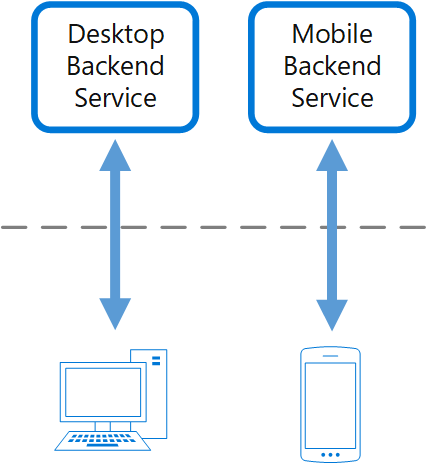
\includegraphics[width=0.45\linewidth]{images/EA/backend-for-frontend.png}
        \caption{Backends for Frontends \\ \cite{EA:Web32}}
        \label{fig:backend-for-frontend}
    \end{figure}

    Wie in Abschnitt \ref{Projektbezug - Anforderungsanalyse} erwähnt, existiert bereits ein Backend für die Desktop-Applikation CGM MAXX. Da diese nicht für den Betrieb auf mobilen Geräten ausgelegt ist, wird im Zuge des Projekts ein Frontend entwickelt, das sich auf mobile Geräte fokussiert. 
    Da die mobile Applikation nur einen Teil der Aufgaben der Desktop-Applikation abdeckt und zusätzlich Funktionen für Kamera und Mikrofon bietet, ist es sinnvoll, ein separates Backend zu entwickeln. So gibt es kein zentrales Backend, das die Anforderungen beider Frontends erfüllen muss, wodurch es zu keinen Konflikten kommen kann. Das bedeutet, dass die Applikationen unabhängig voneinander verändert werden können.
    \cite{EA:Web32}

    \clearpage

    Ein weiteres interessantes Muster ist das \textbf{Compute Resource Consolidation Pattern}.
    Softwaresysteme bestehen oftmals aus mehreren Applikationen, die unabhängig voneinander bereitgestellt werden.
    Dies führt zu einem höheren Bedarf an Computerressourcen, steigenden Bereitstellungskosten und einem größeren Wartungsaufwand. \\

    \begin{figure}[H]
        \centering
        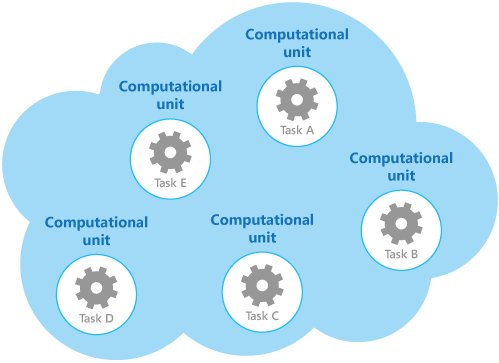
\includegraphics[width=0.55\linewidth]{images/EA/compute-resource-consolidation.png}
        \caption{Vereinfachte Struktur einer cloudbasierten Lösung \\ \cite{EA:Web33}}
        \label{fig:compute-resource-consolidation}
    \end{figure}

    Abbildung \ref{fig:compute-resource-consolidation} zeigt vereinfacht, wie ein verteiltes System in der Cloud aussieht.
    Eine Recheneinheit kann beispielsweise genutzt werden, um ein Microservice zu betreiben.

    In Systemen mit vielen Microservices entstehen jedoch häufig unnötige Kosten, da auf bestimmte Services öfter zugegriffen wird als auf andere. 
    Selbst dann, wenn ein Service gar nicht verwendet wird, entstehen Kosten. Daher ist es wichtig, die Aufteilung der Dienste sorgfältig zu planen, um eine kostengünstige und effiziente Lösung zu schaffen.

    Dieses Muster zielt darauf ab, die \textbf{Auslastung der Recheneinheiten} zu \textbf{erhöhen}, um die \textbf{Kosten für die Ressourcen} zu \textbf{senken}. Erreicht wird dies, indem bestimmte \textbf{Dienste zusammengefasst} und \textbf{auf einer gemeinsamen Recheneinheit betrieben} werden. Außerdem können die Dienste so direkt miteinander kommunizieren, was dazu beiträgt, dass bestimmte Aktionen schneller ausgeführt werden können.

    \textbf{Eingesetzt} wird dieses Muster \textbf{bei Diensten, die die meiste Zeit im Leerlauf verbringen}, um durch das Gruppieren zusammenhängender Einheiten die Kosten zu senken. Weniger geeignet ist für fehlertolerante Vorgänge, da andere Dienste, die auf derselben Recheneinheit betrieben werden, beeinträchtigt werden könnten. \\
    \cite{EA:Web33}

    \clearpage

    Das letzte Entwurfsmuster, das in dieser Arbeit erläutert wird, ist das \textbf{Gateway Routing Pattern}.
    Es kommt zum Einsatz, wenn ein Client innerhalb einer Applikation auf mehrere Dienste zugreift. 
    Dabei fungiert ein \textbf{API-Gateway} als zentraler Kommunikationspunkt, der die \textbf{Anfragen des Clients empfängt} und \textbf{an die entsprechenden Dienste weiterleitet}. Dadurch soll die Komplexität der Kommunikation zwischen dem Client und mehreren Diensten reduziert werden, da der Client nur über einen einzigen Endpunkt mit den Diensten interagiert.
    \cite{EA:Web34}
    
    In Abbildung \ref{fig:gateway-routing} ist das Gateway Routing Pattern dargestellt: 
    
    \begin{figure}[H]
        \centering
        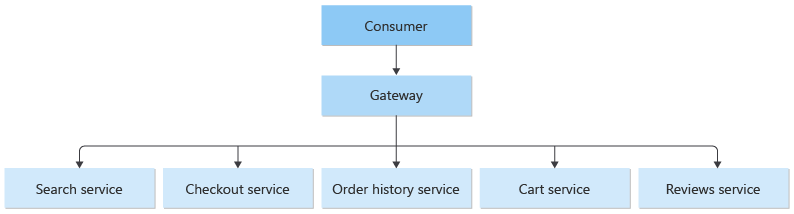
\includegraphics[width=1.05\linewidth]{images/EA/gateway-routing.png}
        \caption{Gatway Routing \\ \cite{EA:Web34}}
        \label{fig:gateway-routing}
    \end{figure}

    Um die Funktionsweise des Musters näher zu verdeutlichen, wird näher auf die Konfiguration des API-Gateways im Projekt CGM MAXX LITE eingegangen. 
    
    In \lil{lst:api-gateway} wird die \textbf{Konfiguration des Gateways} dargestellt:
    \vspace{0.3em}
    \lstinputlisting[
        caption=\texttt{application.yml - API Gateway},
        label=lst:api-gateway,
    ]{sources/EA/application.yml}


    Das API-Gateway lauscht auf den Port 8080 und ermöglicht durch die Definition von Routen den Zugriff auf die dahinterliegenden Microservices. Eine genauere Beschreibung der einzelnen Microservices findet sich in Abschnitt \ref{Projektbezug - Architekturstil}.

     Damit Nutzer/innen diese Services nutzen können, erfolgt der Zugriff über das Frontend. Dabei gibt es eine Konfigurationsdatei mit dem Namen \textbf{environment.ts}, in der spezifische Umgebungsvariablen gesetzt werden können. In \lil{lst:frontend-environment-variables} werden die URLs für den Zugriff auf das Patient Service und File Service festgelegt. Beide greifen dabei auf den Port 8080 zu, also auf das API Gateway, das die Anfragen an die entsprechenden Microservices weiterleitet: \\

    \lstinputlisting[
        caption=\texttt{environment.ts},
        label=lst:frontend-environment-variables,
        firstline=5,
        lastline=10
    ]{sources/EA/environment.ts}


    % --- D E V O P S  ---

    \subsubsection{DevOps und Automatisierung} \label{DevOps}

    Nachdem die Rolle von Entwurfsmustern in der Cloud erklärt wurde, wird im Anschluss der Prozess der Bereitstellung thematisiert.
    
    Der Begriff DevOps ist eine \textbf{Abkürzung für Development Operations}. Es handelt sich dabei um eine Entwicklungsmethodik, die es ermöglicht, die Bereitstellung von Software zu beschleunigen, indem bestimmte \textbf{Arbeitsschritte automatisiert} und die Zusammenarbeit zwischen dem Entwicklungsteam und IT-Operations-Team\footnote{Personen, die für die Bereitstellung von IT-Services verantwortlich sind} gefördert wird.
    \cite{EA:Web35}

    DevOps bietet die Möglichkeit, nicht nur alle paar Monate neue Änderungen zu veröffentlichen, wie es vor einigen Jahren noch der Fall war, sondern sogar mehrmals am Tag neue Releases bereitzustellen. 
    \cite{EA:Web36}
    
    Zusätzlich bietet DevOps weitere Vorteile:
    \begin{itemize}
        \item Bessere Qualität der Software
        \item Effizienteres Arbeiten durch die Zusammenarbeit sonst isolierter Teams
        \item Wettbewerbsvorteil durch die schnelle Bereitstellung neuer Funktionen
    \end{itemize}

    Wie zu Beginn bereits erwähnt, geht es darum, Software schneller ausliefern zu können. Allerdings bezieht sich dies nicht nur auf die Bereitstellung. 
    Damit Software schneller auf den Markt gebracht werden kann, müssen auch die vorhergehenden Phasen berücksichtigt werden.
    Dieser \textbf{iterative und automatisierte Prozess} wird als \textbf{Lebenszyklus} bezeichnet.
    \cite{EA:Web35}

    \begin{figure}[H]
        \centering
        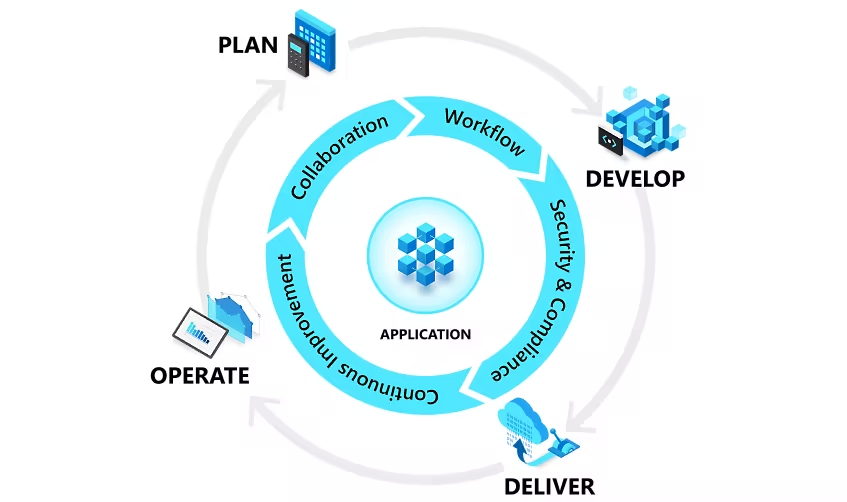
\includegraphics[width=0.9\linewidth]{images/EA/devops-lifecycle.png}
        \caption{DevOps-Lebenszyklus \\ \cite{EA:Web37}}
        \label{fig:devops-lifecycle}
    \end{figure}
      
    In Abbildung \ref{fig:devops-lifecycle} wird dargestellt, wie der DevOps-Lebenszyklus aussieht.
    Der Prozess \textbf{beginnt mit der Planung}. Dabei wird festgelegt, welche Funktionalitäten im nächsten Sprint umgesetzt werden sollen, um Kund/innen einen Mehrwert zu bieten. Hierbei wird auf \textbf{agiles Projektmanagement} gesetzt, um auf das Feedback der Anwender/innen einzugehen und falls gewünscht, entsprechende Änderungen vorzunehmen.
    
    Nachdem die Planung abgeschlossen ist, kann mit der \textbf{Entwicklung} begonnen werden. Neben der Implementierung neuer Funktionalitäten und der Behebung von Bugs wird der geschriebene Code auch getestet (siehe Kapitel \ref{}). Bevor eine neue Version der Software bereitgestellt wird, sollte diese vorher ausgiebig getestet werden. Dazu werden automatische Tests durchlaufen und anschließend kann die Software automatisch ausgeliefert werden. Realisiert wird dies mithilfe von CI/CD\footnote{Continuous Integration and Continuous Delivery}, das im Anschluss kurz beschrieben wird. Eine genauere Beschreibung kann in Kapitel \ref{} gefunden werden.

    \clearpage

    Die nächste Phase befasst sich mit der \textbf{Bereitstellung}. Dabei sollen entsprechende Anwendungen zuverlässig in einer Produktionsumgebung bereitgestellt werden. Dazu gehört auch die Konfiguration und Verwaltung der Infrastruktur, was beispielsweise mit Infrastructure as Code (IaC) erreicht werden kann. Dies wird im Abschnitt \ref{IaC} näher beschrieben.

    Treten in der Produktionsumgebung keine Fehler auf, so kann die Software für die Nutzer/innen zugänglich gemacht werden. Diese Phase bezeichnet man als \textbf{Ausführungsphase}. Die Software wird dabei überwacht und im Falle eines Fehlers wird versucht, diesen zu beheben. 

    Dieser Prozess wiederholt sich und trägt dazu bei, dass das \textbf{DevOps-Team kontinuierlich dazulernt} und somit bessere Ergebnisse liefern kann.
    \cite{EA:Web35, EA:Web37}

    Damit einzelne Phasen automatisiert und optimiert werden können, gibt es verschiedene Möglichkeiten, die eingesetzt werden können.
    Eine davon ist CI/CD. Dabei handelt es sich um eine Kombination aus kontinuierlicher Integration (Continuous Integration) und kontinuierlicher Lieferung (Continuous Delivery). Dadurch wird neuer Code ausgeliefert, ohne diesen manuell bereitstellen zu müssen.

    Die \textbf{kontinuierliche Integration (CI)} sorgt dafür, dass der Code eines bestimmten Branches, in der Regel des main-Branches, bei jedem neuen Commit getestet wird, indem die Anwendung gebaut wird.

    \begin{figure}[H]
        \centering
        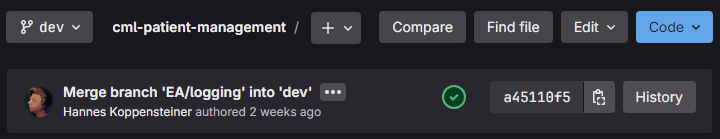
\includegraphics[width=1\linewidth]{images/EA/cml-ci-passed.png}
        \caption{Erfolgreicher Build - CGM MAXX LITE}
        \label{fig:cml-ci-passed}
    \end{figure}

    Abbildung \ref{fig:cml-ci-passed} zeigt einen Ausschnitt aus einem \textbf{GitLab-Repository}, das den erfolgreichen CI-Build eines Projekts dokumentiert.
    Im gezeigten Beispiel handelt es sich um den Microservice zur Verwaltung von Patientendaten. Sobald neue Änderungen am dev-Branch vorgenommen werden, wird versucht, die Anwendung zu bauen. In diesem Fall wurde Logging zur Anwendung hinzugefügt. Der grüne Haken auf der rechten Seite symbolisiert den erfolgreichen Build-Prozess.

    Sobald der CI-Prozess abgeschlossen ist, sorgt die \textbf{kontinuierliche Lieferung (CD)} dafür, dass die Software so vorbereitet wird, dass sie jederzeit bereitgestellt werden kann.
    \cite{EA:Web38}
    

    % --- I N F R A S T R U C T U R E   A S   C O D E ---    

    \subsubsection{Infrastructure as Code (IaC)} \label{IaC}

    Infrastructure as Code (IaC) ist eine \textbf{in DevOps angewandte Methode}, die insbesondere \textbf{in der kontinuierlichen Bereitstellung von Software Anwendung findet}. \\
    Dabei wird Code geschrieben, der es ermöglicht, die Infrastruktur automatisch zu konfigurieren und bereitzustellen, 
    sodass manuelle Eingriffe vermieden werden. \\
    \cite{EA:Web37}

    Diese Methode eignet sich daher besonders gut, um \textbf{komplexe und umfangreiche Umgebungen} bereitzustellen, die häufig aufgesetzt werden müssen. Dazu zählen unter anderem Entwicklungs- und Test-Umgebungen. \\
    \cite{EA:Web30, EA:Web39}
    
    IaC bietet dabei einige Vorteile:
    \begin{itemize}
        \item Umgebungen können einfach dupliziert werden
        \item Weniger Fehler durch automatische Erstellung
        \item Schnelle und zuverlässige Bereitstellung
    \end{itemize}

    Um Infrastruktur mithilfe von Code zu erzeugen, gibt es zwei verschiedene Ansätze:
    \begin{itemize}
        \item \textbf{Deklarativer Ansatz}
        \begin{itemize}[label=$\circ$]
            \item Der gewünschte Endzustand des Systems wird durch die \\ Definition von Ressourcen und deren Einstellungen beschrieben.
        \end{itemize}
        
        \item \textbf{Imperativer Ansatz}
        \begin{itemize}[label=$\circ$]
            \item Der gewünschte Endzustand wird durch die Beschreibung aller \\ notwendigen Schritte zur Konfiguration der Ressourcen erreicht.
        \end{itemize}
    \end{itemize}

    Damit die oben genannten Vorteile realisiert werden können, stehen zahlreiche Tools von verschiedenen Herstellern zur Verfügung. \cite{EA:Web40} \\
    Zu den bekanntesten IaC-Tools gehören: 
    \begin{itemize}
        \item Terraform
        \item AWS CloudFormation
        \item Ansible
    \end{itemize}

    Neben den genannten Tools existieren zahlreiche weitere Werkzeuge, die für die Erstellung und Verwaltung von Infrastruktur genutzt werden können.
     Da sich all diese Tools in bestimmten Punkten unterscheiden, ist es wichtig, ein für den Anwendungsfall passendes Werkzeug auszuwählen.

    Um die Unterschiede der genannten IaC-Tools zu verdeutlichen, werden diese in Tabelle \ref{tab:iac-tools} miteinander verglichen:

    \begin{table}[H]
        \centering
        \begin{tabular}{|l|c|c|c|}
        \hline
        \textbf{Kriterium} & \textbf{Terraform} & \textbf{CloudFormation} & \textbf{Ansible}\\ \hline
        Anbieter & HashiCorp & Amazon Web Services & Red Hat \\ \hline
        Ansatz & Deklarativ & Deklarativ & Deklarativ/imperativ \\ \hline
        Konfigurationssprache & HCL/JSON & YAML/JSON & YAML \\ \hline
        Multi-Provider-Support & Ja & Nein & Ja \\ \hline
        Kosten und Lizenzierung & Kostenlos & AWS-Ressourcen & Kostenlos \\ \hline
        \end{tabular}
        \caption{IaC-Tools}
        \label{tab:iac-tools}
    \end{table}

    Im weiteren Verlauf wird erklärt, wofür die einzelnen Tools verwendet werden, und wie sie sich in ihrer Funktionsweise unterscheiden.
    \cite{EA:Web41, EA:Web42, EA:Web43} \\


    % --- T E R R A F O R M ---
    
    \textbf{Terraform}

    Terraform ist ein von HashiCorp entwickeltes Tool für Infrastructure as Code (IaC), das die Bereitstellung und Verwaltung von Infrastruktur sowohl in Cloud-Umgebungen als auch On-Premise ermöglicht. Geschrieben werden die Konfigurationsdateien in der HashiCorp Configuration Language (HCL) oder in JSON, die beide eine simple und leicht verständliche Struktur aufweisen.
    
    Ein wesentlicher Vorteil von Terraform ist die Unterstützung zahlreicher \\Cloud-Dienstanbieter, darunter AWS, Azure und Google Cloud Platform. \\ \cite{EA:Web44}
    
    \begin{figure}[H]
        \centering
        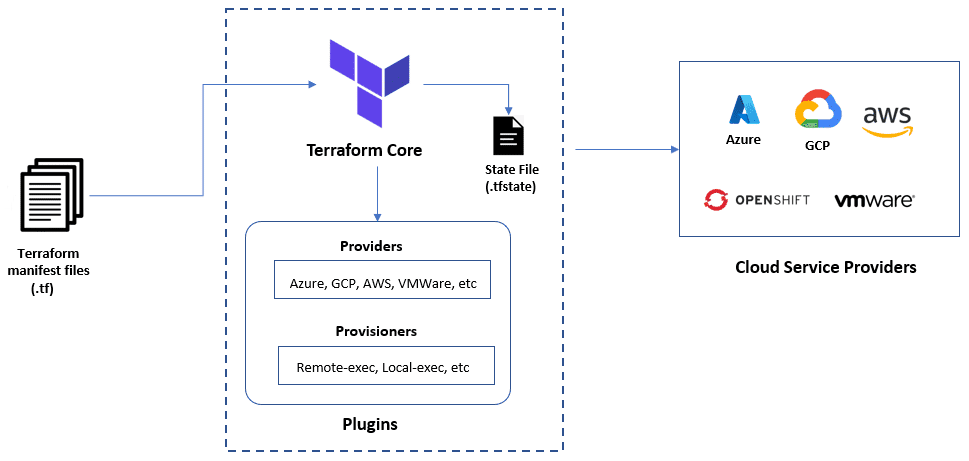
\includegraphics[width=1\linewidth]{images/EA/terraform-architecture.png}
        \caption{Terraform Architektur \\ \cite{EA:Web49}}
        \label{fig:terraform-architecture}
    \end{figure}

    Abbildung \ref{fig:terraform-architecture} veranschaulicht die grundlegende Architektur von Terraform.
    Der Prozess beginnt mit dem Erstellen einer Konfigurationsdatei, in der alle notwendigen Einstellungen vorgenommen werden, um den gewünschten Endzustand des Systems zu erreichen. Anschließend wird mithilfe der \textbf{Terraform CLI\footnote{Command-line Interface}} ein Ausführplan erstellt. Erst wenn dieser bestätigt wird, werden die Änderungen durchgeführt.

    Die Terraform CLI, auch Terraform Core genannt, ist das zentrale Werkzeug für die Verwaltung von Infrastruktur.
    Weiters interagiert sie mit \textbf{Providern}, die die Kommunikation mit unterschiedlichen Diensten ermöglichen. Dabei werden die vorliegenden Konfigurationen in die für den Dienstanbieter vorgesehenen API Calls umgewandelt und passen die Einstellungen entsprechend an. \\
    \cite{EA:Web44, EA:Web49}

    \clearpage

    % --- A W S   C L O U D F O R M A T I O N ---

    \textbf{AWS CloudFormation}

    Wie der Name bereits andeutet, handelt es sich um einen Dienst von Amazon Web Services, der speziell auf die \textbf{Bereitstellung von AWS-Ressourcen} ausgerichtet ist. Der Dienst selbst ist kostenlos. Es entstehen lediglich Kosten für die bereitgestellten Ressourcen, wie beispielsweise EC2-Instanzen.

    In Abbildung \ref{fig:aws-cloudformation} wird der Ablauf der Bereitstellung gezeigt:

    \begin{figure}[H]
        \centering
        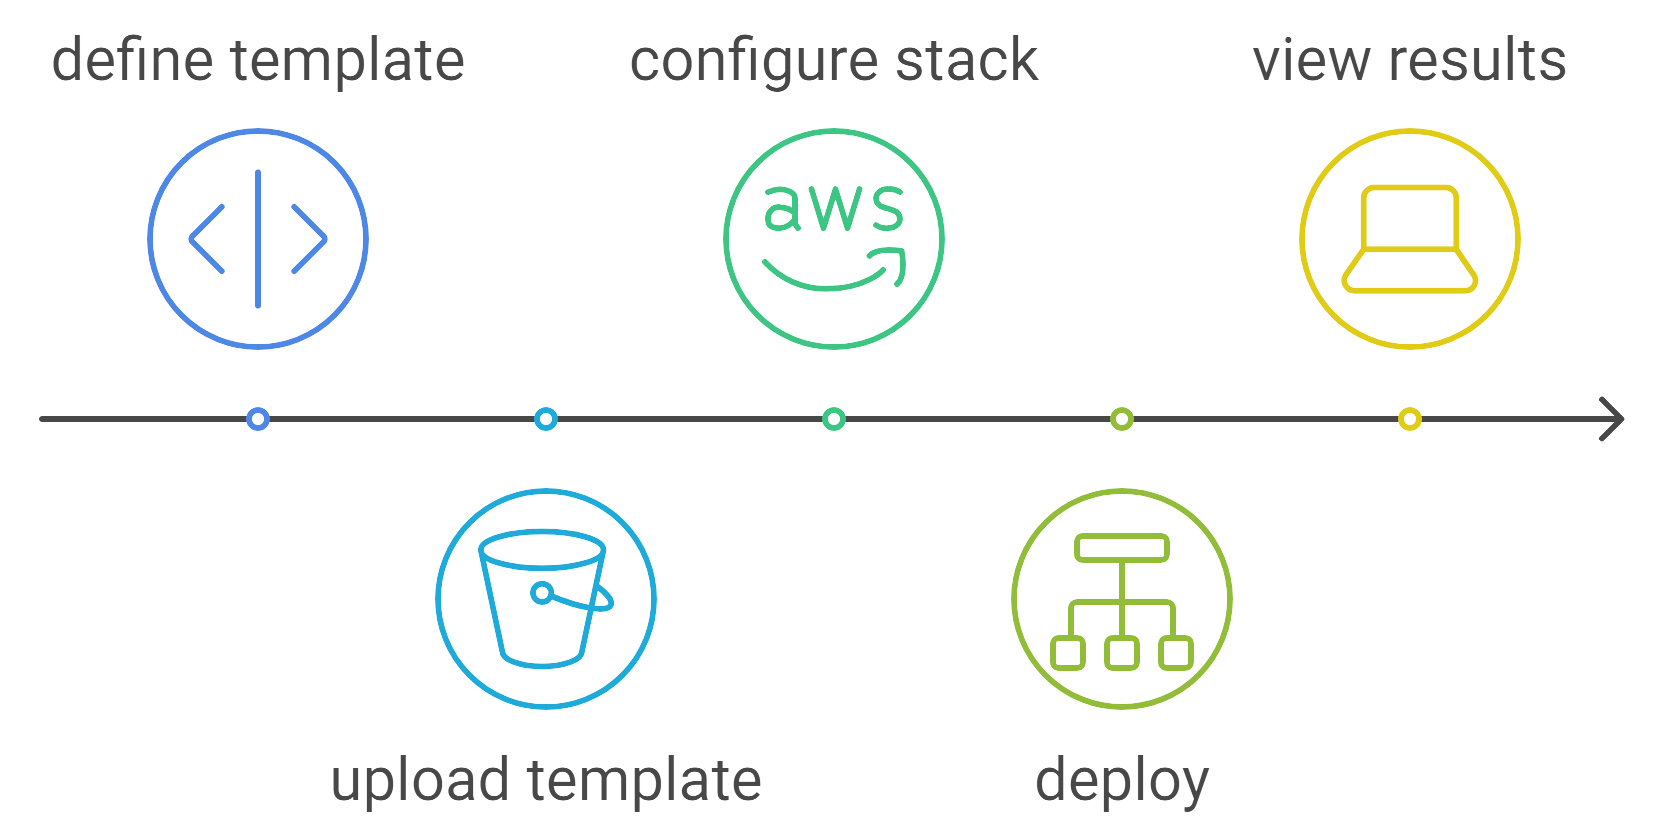
\includegraphics[width=0.7\linewidth]{images/EA/cloudformation-workflow.png}
        \caption{AWS CloudFormation Funktionsweise}
        \label{fig:aws-cloudformation}
    \end{figure}

    Ähnlich wie bei Terraform, muss auch bei CloudFormation eine \textbf{Vorlage} erstellt werden, welche die benötigten Ressourcen beschreibt.
    Bei der Konfigurationssprache kann entweder YAML oder JSON eingesetzt werden. Alle Ressourcen, die in einer Vorlage definiert werden, werden als eine Einheit betrachtet, die auch als \textbf{Stack} bezeichnet wird.

    Um die Änderungen einer Vorlage zu übernehmen, muss ein \textbf{Änderungssatz} erstellt werden. Dabei wird auf den Speicherort der ausgewählten Vorlage verwiesen, die entweder \textbf{lokal oder in einem Amazon S3-Bucket abgespeichert} werden kann. 
    Der Änderungssatz zeigt dabei, welche Änderungen vorgenommen werden und ähnelt somit einem Ausführungsplan in Terraform. 
    \cite{EA:Web50, EA:Web51}
    
    Der Unterschied zwischen diesen beiden Tools besteht darin, dass wenn in CloudFormation ein Fehler beim Änderungsvorgang auftritt, der Stack auf den letzten funktionsfähigen Stand zurückgesetzt wird. In Terraform hingegen werden nur die Ressourcen isoliert, die vom Fehler betroffen sind. Zudem unterstützt Terraform neue AWS-Funktionen oft schneller als CloudFormation selbst. 
    \cite{EA:Web52}

    \clearpage


    % --- R E D   H A T   A N S I B L E ---

    \textbf{Ansible}    

    Ansible ist kein IaC-Tool im eigentlichen Sinne. Es ist vielmehr ein Konfigurationswerkzeug, das sich auf die Automatisierung unterschiedlicher Tasks fokussiert. Dazu zählen unter anderem Systemupdates, die Installation von Software, das Einrichten einer Firewall, und vieles mehr. Um dies zu realisieren, werden sogenannte \textbf{Playbooks} eingesetzt, die in der Datenserialisierungssprache YAML geschrieben werden.

    Während Terraform besser für die Bereitstellung von Infrastruktur geeignet ist, spielt Ansible seine Stärken bei der Konfigurationsverwaltung aus. Beide Werkzeuge haben ihre Vor- und Nachteile. In der Praxis werden Terraform und Ansible häufig kombiniert, 
    um die Stärken beider Tools optimal zu nutzen.
    \cite{EA:Web45, EA:Web48}
    
    \begin{figure}[H]
        \centering
        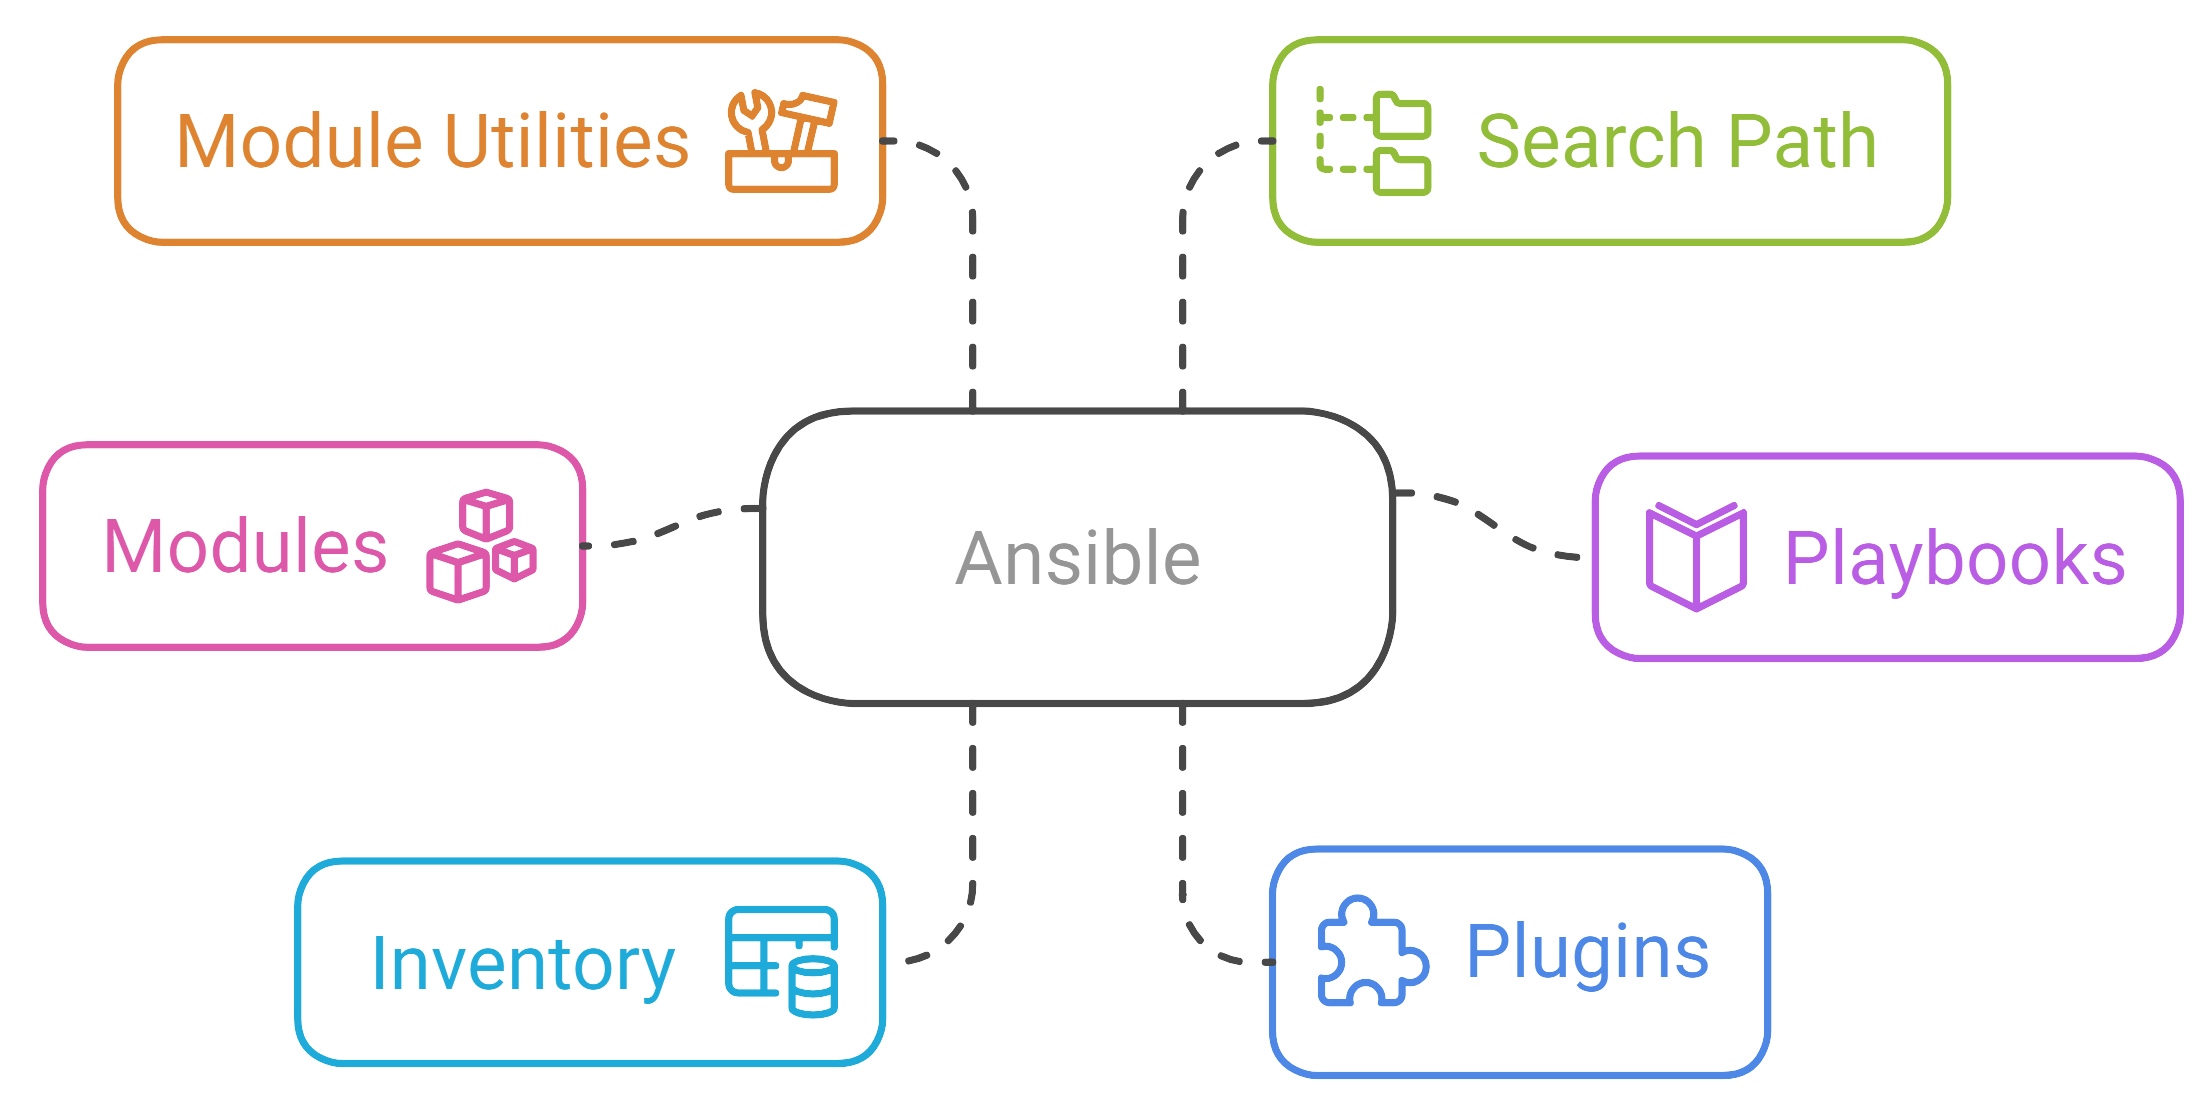
\includegraphics[width=0.7\linewidth]{images/EA/ansible-architecture.png}
        \caption{Ansible Architektur}
        \label{fig:ansible-architecture}
    \end{figure}

    Um die Funktionsweise von Ansible besser zu verstehen, wird die Architektur anhand der Grafik in Abbildung \ref{fig:ansible-architecture} näher erklärt. Diese setzt sich aus folgenden Komponenten zusammen:

    \begin{itemize}
        \item \textbf{Modules}
        \begin{itemize}[label=$\circ$]
            \item Skripte, die auf Managed Nodes\footnote{Geräte, die von Ansible verwaltet werden} kopiert und dort ausgeführt werden
            \item Standardmäßig erfolgt die Ausführung über SSH
            \item Erledigen die in den Playbooks definierten Tasks
        \end{itemize}
        
        \item \textbf{Module Utilities}
        \begin{itemize}[label=$\circ$]
            \item Mehrfach vorkommende identische Codeausschnitte werden gespeichert
            \item Redundanter Code wird vermieden und die Wartung wird erleichtert
        \end{itemize}
        
        \item \textbf{Plugins}
        \begin{itemize}[label=$\circ$]
            \item Ergänzt Ansible um neue Funktionen
            \item Eigene Plugins können mithilfe von Python geschrieben werden
        \end{itemize}
        
        \item \textbf{Playbooks}
        \begin{itemize}[label=$\circ$]
            \item YAML-Dateien für die Konfiguration von Managed Nodes
            \item Einfach zu lesen
        \end{itemize}
        
        \item \textbf{Inventory}
        \begin{itemize}[label=$\circ$]
            \item Liste mit den Managed Nodes, die durch Ansible verwaltet werden
            \item Gruppierung von Hostnamen und IP-Adressen möglich
            
        \end{itemize}
        
        \item \textbf{Search Path}
        \begin{itemize}[label=$\circ$]
            \item Gibt an, wo benötigte Module, Plugins, Playbooks, usw. zu finden sind
        \end{itemize}
        
    \end{itemize}
    \cite{EA:Web46, EA:Web47} \\


    % --- I N F R A S T R U C T U R E   A S   C O D E   -   A B S C H L U S S ---

    Abschließend lässt sich sagen, dass es nicht das eine \glqq{perfekte}\grqq\ Werkzeug gibt. 
    Daher ist es wichtig, den genauen Anwendungsfall zu kennen, um auf dieser Grundlage ein passendes Tool auszuwählen.
    Das Ziel sollte sein, eine einfache und schnelle Lösung zu finden, um Infrastruktur und/oder Software bereitzustellen und so einen Wettbewerbsvorteil zu erzielen.

    Zudem wird der Entwicklungsprozess erleichtert, da durch die einfache Reproduzierbarkeit von Systemen weniger Fehler auftreten.
    Auf diese Weise können sich die Entwickler/innen auf ihre eigentlichen Aufgaben konzentrieren, ohne stundenlang nach der Ursache eines Fehlers suchen zu müssen.

    \clearpage

    \section{Fazit und Ausblick} \label{Fazit und Ausblick}
    % --- A B S C H L U S S ---

Bevor die Erkenntnisse, die im Laufe dieser Arbeit gewonnen wurden, zusammengefasst werden, soll ein letztes Mal darauf hingewiesen werden, dass die behandelten Themen bei Weitem nicht alle Teile der Softwarearchitektur abdecken.
Das Ziel dieser Arbeit ist es, die Bedeutung der Softwarearchitektur hervorzuheben und zu vermitteln, dass sie weit mehr als nur die Implementierung von sauberem Quellcode umfasst.

Softwarearchitektur befasst sich mit dem gesamten Lebenszyklus des Systems, beginnend bei der Planung bis hin zum Betrieb.


    % --- Z U S A M M E N F A S S U N G   D E R   E R G E B N I S S E ---
    
    \subsection{Zusammenfassung der Ergebnisse}
    
    Bei der Softwarearchitektur handelt es sich nicht nur um einen Bauplan, der angibt, wie ein Softwaresystem aufgebaut ist und wie die einzelnen Bestandteile miteinander interagieren. Es ist auch ein wichtiges Instrument für die Kommunikation. Durch verschiedene Formen der Darstellung, die in Abschnitt \ref{Architekturmodellierung} näher beschrieben werden, können Grafiken erzeugt werden, die verwendet werden können, um mit verschiedenen Stakeholdern zu kommunizieren. 

    Um eine Softwarearchitektur zu entwerfen, die den Wünschen der Kund/innen entspricht, spielt die Anforderungsanalyse (siehe \ref{Anforderungsanalyse}) eine entscheidende Rolle. Durch die Definition funktionaler und nicht-funktionaler Anforderungen wird festgelegt, was die Software können soll, um die Nutzer/innen zufriedenzustellen.  

    Die Ergebnisse der Anforderungsanalyse dienen dabei als Entscheidungsgrundlage für den zugrundeliegenden Architekturstil (siehe \ref{Architekturstile}). Je nachdem, was die Anforderungen sind, eignen sich bestimmte Stile besser als andere, wobei auch hier jeder Stil seine Vor- und Nachteile hat.

    Da sich diese Arbeit hauptsächlich auf cloudbasierte Anwendungen fokussiert, kann es von Relevanz sein, grundlegende Entwurfsmuster für die Cloud (siehe Abschnitt \ref{Entwurfsmuster für die Cloud}) zu kennen, um häufig auftretenden Problemen zu entweichen. Zudem gibt es heutzutage bereits einige Möglichkeiten, um die Entwicklung und Bereitstellung von Software zu beschleunigen. Methoden wie DevOps (siehe Abschnitt \ref{DevOps}) werden immer bedeutender und ermöglichen es, Releases schneller und einfacher zu veröffentlichen, was einen Wettbewerbsvorteil schaffen kann.

    \clearpage

    Blickt man nun auf die Ergebnisse des Projekts CGM MAXX LITE, so wurden alle Grundfunktionalitäten erfolgreich umgesetzt und erfüllen die Erwartungen des Auftraggebers. Die Softwarearchitektur ist so konzipiert, dass das System in Zukunft einfach erweitert und angepasst werden kann. 
    Um für hohe Leistung zu sorgen, wurde die Kommunikation zwischen Frontend und Backend so gestaltet, dass nur notwendige Daten übertragen werden.
    Beim gewählten Architekturstil handelt es sich um eine Microservices-Architektur, die gewährleisten soll, dass wenn ein Service ausfällt, übrige Services des Systems weiterhin zur Verfügung stehen. Dadurch ist sichergestellt, dass im Falle eines Fehlers nur bestimmte Teile des Systems vorübergehend nicht erreichbar sind.
    Wie die Architektur aussieht, kann mithilfe des Container-Diagramms in Abbildung \ref{fig:c4-container-diagram} dargestellt werden.
    
    Durch das Hinzufügen einer CI/CD-Pipeline wird nach jeder Änderung am dev-Branch geprüft, ob die Applikation erfolgreich gebaut werden kann und wird anschließend am Portainer bereitgestellt, wodurch das System von überall aus getestet und dem Auftraggeber präsentiert werden kann.
    Zusätzlich wird das Frontend durch ESLint überprüft, was in Abschnitt \ref{} genauer thematisiert wird.

    Da es sich um die Entwicklung einer Arztsoftware handelt, bei der mit sensiblen Daten gearbeitet wird und Zuverlässigkeit, Fehlertoleranz sowie Sicherheit gewährleistet sein müssen, werden neben einfachen Unit-Tests auch End-To-End-Tests geschrieben, die testen, ob die Benutzeroberfläche korrekt funktioniert. Darauf wird in Kapitel \ref{} näher eingegangen.

    Wie die Benutzeroberfläche der mobilen Arztsoftware schlussendlich aussieht, wird in Kapitel \ref{} gezeigt.
    Dabei liegt der Fokus auf einer benutzerfreundlichen Oberfläche, die leicht bedient werden kann, um alltägliche Arbeitsabläufe zu beschleunigen.

    
    % --- Z U K Ü N F T I G E   E N T W I C K L U N G E N ---
    
    \subsection{Zukünftige Entwicklungen}

    Wie bereits zu Beginn der Arbeit erwähnt, ist die Softwarearchitektur dynamisch und entwickelt sich ständig weiter, weshalb es schwierig ist vorherzusagen, wohin sich die Architektur von Software in Zukunft entwickeln wird. Dennoch ist klar, dass Cloud Computing und die zunehmende Verlagerung von Anwendungen in die Cloud eine immer zentralere Rolle spielen werden.

    Trotz all dieser Veränderungen wird sich an einer Sache nichts ändern: Eine gut durchdachte Softwarearchitektur ist maßgeblich für den Erfolg eines Softwaresystems verantwortlich. Deswegen ist es wichtig, sich kontinuierlich mit neuen Technologien und Entwurfsmustern zu beschäftigen, um mit der Konkurrenz mithalten zu können.

\clearpage
%\input{textparts/OB/...}
\clearpage
%\input{textparts/HK/...}
\clearpage
 
%--------------------------------------------------------------------------
% Anhang
%--------------------------------------------------------------------------
   
    \addcontentsline{toc}{chapter}{Anhang}
    \phantomsection
    
	\addcontentsline{toc}{section}{Abbildungsverzeichnis}
	\listoffigures
	\cleardoublepage
	\phantomsection
	
	\addcontentsline{toc}{section}{Tabellenverzeichnis}
	\listoftables
	\cleardoublepage
	\phantomsection

	\addcontentsline{toc}{section}{Verzeichnis der Listings}
	\lstlistoflistings
	\cleardoublepage
	\phantomsection
	
	%\addcontentsline{toc}{section}{Index}
    %\printindex
    %\cleardoublepage
    %\phantomsection
  
	\addcontentsline{toc}{section}{Literaturverzeichnis}
	%\bibliographystyle{alpha} 		 %Standardstyle
	%\bibliographystyle{dinat}		 %Style und Layout nach DIN 1502
	%\bibliography{tiger}					 %Literaturverzeichnis einfügen
	\begin{thebibliography}{999}

    \bibitem[EA:Book01]{EA:Book01}
    Robert C. Martin: \\
        \emph{Clean Architecture: A Craftsman's Guide to Software Structure and Design} \\
        Pearson Education Inc., 2018 \\
        ISBN: 978-0-13-449416-6

    \bibitem[EA:Book02]{EA:Book02}
    Mark Richards \& Neal Ford: \\
        \emph{Handbuch moderner Softwarearchitektur} \\
        O'Reilly, 2021 \\
        ISBN: 978-3-96009-149-3

    \bibitem[EA:Book03]{EA:Book03}
    Len Bass, Paul Clements, Rick Kazman: \\
        \emph{Software Architecture in Practise} \\
        Addison-Wesley Professional, 2003 \\
        ISBN: 978-0321154958

    \bibitem[EA:Web01]{EA:Web01}
    \href{https://leanpub.com/software-architecture-for-developers/read}{https://leanpub.com/software-architecture-for-developers/read} \\
    Definition der Softwarearchitektur \\
    19.10.2024

    \bibitem[EA:Web02]{EA:Web02}
    \href{https://thestory.is/en/process/development-phase/software-architecture/}{https://thestory.is/en/process/development-phase/software-architecture/} \\
    Aufgaben und Ziele der Softwarearchitektur \\
    29.10.2024

    \bibitem[EA:Web03]{EA:Web03}
    \href{https://www.redhat.com/en/blog/what-is-software-architect}{https://www.redhat.com/en/blog/what-is-software-architect} \\
    Aufgaben des Softwarearchitekten \\
    29.10.2024 

    \bibitem[EA:Web04]{EA:Web04}
    \href{https://www.geeksforgeeks.org/functional-vs-non-functional-requirements}{https://www.geeksforgeeks.org/functional-vs-non-functional-requirements} \\
    Funktionale und nicht-funktionale Anforderungen \\
    02.11.2024

    \clearpage

    \bibitem[EA:Web05]{EA:Web05}
    \href{https://www.geeksforgeeks.org/software-engineering-classification-of-software-requirements}{https://www.geeksforgeeks.org/software-engineering-classification-of-software-requirements} \\
    Anforderungsanalyse \\
    02.11.2024

    \bibitem[EA:Web06]{EA:Web06}
    \href{https://en.wikipedia.org/wiki/Agile_software_development}{https://en.wikipedia.org/wiki/Agile-software-development} \\
    Agile Softwareentwicklung \\
    02.11.2024

    \bibitem[EA:Web07]{EA:Web07}
    \href{https://www.studysmarter.de/ausbildung/ausbildung-in-it/fachinformatiker-anwendungsentwicklung/funktionale-anforderungen}{https://www.studysmarter.de/ausbildung/ausbildung-in-it/fachinformatiker-anwendungsentwicklung/funktionale-anforderungen} \\
    Funktionale Anforderungen \\
    02.11.2024 

    \bibitem[EA:Web08]{EA:Web08}
    \href{https://www.ibm.com/docs/en/aix/7.1?topic=implementation-performance-requirements-documentation}{https://www.ibm.com/docs/en/aix/7.1?topic=implementation-performance-requirements-documentation} \\
    Nicht-funktionale Anforderungen - Performance \\
    16.11.2024

    \bibitem[EA:Web09]{EA:Web09}
    \href{https://www.geeksforgeeks.org/recovery-testing-in-software-testing}{https://www.geeksforgeeks.org/recovery-testing-in-software-testing} \\
    Nicht-funktionale Anforderungen - Recovery Testing \\
    16.11.2024

    \bibitem[EA:Web10]{EA:Web10}
    \href{https://www.cgm.com/aut_de/produkte/arztpraxis/cgm-maxx.html}{https://www.cgm.com/aut-de/produkte/arztpraxis/cgm-maxx.html} \\
    CGM MAXX \\
    22.11.2024

    \bibitem[EA:Web11]{EA:Web11}
    \href{https://www.franchiseportal.at/definition/unternehmensvision-a-4974}{https://www.franchiseportal.at/definition/unternehmensvision-a-4974} \\
    Vision \\
    11.12.2024 \\

    \bibitem[EA:Web12]{EA:Web12}
    \href{https://medium.com/@alastairallen/visualising-software-architecture-why-its-important-and-how-i-do-it-5c2f4b65b31a}{https://medium.com/@alastairallen/visualising-software-architecture-why-its-important-and-how-i-do-it-5c2f4b65b31a} \\
    Architekturmodellierung \\
    18.12.2024 \\

    \bibitem[EA:Web13]{EA:Web13}
    \href{https://miro.com/diagramming/what-is-software-architecture-diagramming}{https://miro.com/diagramming/what-is-software-architecture-diagramming} \\
    Softwarearchitektur - Diagramme \\
    18.12.2024 \\

    \clearpage

    \bibitem[EA:Web14]{EA:Web14}
    \href{https://www.sciencedirect.com/topics/computer-science/architecture-model}{https://www.sciencedirect.com/topics/computer-science/architecture-model} \\
    Architekturmodellierung \\
    22.12.2024 \\

    \bibitem[EA:Web15]{EA:Web15}
    \href{https://www.studysmarter.de/studium/informatik-studium/softwareentwicklung/softwarearchitektur}{https://www.studysmarter.de/studium/informatik-studium/softwareentwicklung/softwarearchitektur} \\
    Architekturentwurf \\
    23.12.2024 \\

    \bibitem[EA:Web16]{EA:Web16}
    \href{https://www.redhat.com/en/blog/software-architecture-tips}{https://www.redhat.com/en/blog/software-architecture-tips} \\
    Architekturentwurf \\
    23.12.2024 \\

    \bibitem[EA:Web17]{EA:Web17}
    \href{https://miro.com/blog/uml-diagram}{https://miro.com/blog/uml-diagram} \\
    UML-Diagramme \\
    23.12.2024 \\

    \bibitem[EA:Web18]{EA:Web18}
    \href{https://www.geeksforgeeks.org/unified-modeling-language-uml-introduction}{https://www.geeksforgeeks.org/unified-modeling-language-uml-introduction} \\
    UML-Diagramme \\
    23.12.2024 \\

    \bibitem[EA:Web19]{EA:Web19}
    \href{https://miro.com/de/diagramm/was-ist-ein-uml-diagramm}{https://miro.com/de/diagramm/was-ist-ein-uml-diagramm} \\
    UML-Diagramme \\
    23.12.2024 \\

    \bibitem[EA:Web20]{EA:Web20}
    \href{https://t2informatik.de/en/smartpedia/behavior-diagram}{https://t2informatik.de/en/smartpedia/behavior-diagram} \\
    Verhaltensdiagramme \\
    27.12.2024 \\

    \bibitem[EA:Web21]{EA:Web21}
    \href{https://www.visual-paradigm.com/guide/uml-unified-modeling-language/uml-class-diagram-tutorial}{https://www.visual-paradigm.com/guide/uml-unified-modeling-language/uml-class-diagram-tutorial} \\
    Klassendiagramme \\
    27.12.2024 \\

    \clearpage

    \bibitem[EA:Web22]{EA:Web22}
    \href{https://www.freecodecamp.org/news/a-quick-intro-to-dependency-injection-what-it-is-and-when-to-use-it-7578c84fa88f}{https://www.freecodecamp.org/news/a-quick-intro-to-dependency-injection-what-it-is-and-when-to-use-it-7578c84fa88f} \\
    Dependency Injection \\
    27.12.2024 \\

    \bibitem[EA:Web23]{EA:Web23}
    \href{https://www.visual-paradigm.com/guide/uml-unified-modeling-language/what-is-sequence-diagram}{https://www.visual-paradigm.com/guide/uml-unified-modeling-language/what-is-sequence-diagram} \\
    Sequenzdiagramm \\
    27.12.2024 \\

    \bibitem[EA:Web24]{EA:Web24}
    \href{https://www.lucidchart.com/pages/de/uml-sequenzdiagramme}{https://www.lucidchart.com/pages/de/uml-sequenzdiagramme} \\
    Sequenzdiagramm \\
    27.12.2024 \\

    \bibitem[EA:Web25]{EA:Web25}
    \href{https://www.freecodecamp.org/news/how-to-create-software-architecture-diagrams-using-the-c4-model}{https://www.freecodecamp.org/news/how-to-create-software-architecture-diagrams-using-the-c4-model} \\
    C4-Modell \\
    30.12.2024 \\

    \bibitem[EA:Web26]{EA:Web26}
    \href{https://miro.com/de/diagramm/was-ist-das-c4-model-in-software-architektur}{https://miro.com/de/diagramm/was-ist-das-c4-model-in-software-architektur} \\
    C4-Modell \\
    30.12.2024 \\

    \bibitem[EA:Web27]{EA:Web27}
    \href{https://www.lucidchart.com/blog/c4-model}{https://www.lucidchart.com/blog/c4-model} \\
    C4-Modell \\
    31.12.2024 \\

    \bibitem[EA:Web28]{EA:Web28}
    \href{https://c4model.com/diagrams}{https://c4model.com/diagrams} \\
    C4-Modell - Diagramme \\
    31.12.2024 \\

    \bibitem[EA:Web29]{EA:Web29}
    \href{https://c4model.com/diagrams/component}{https://c4model.com/diagrams/component} \\
    C4-Modell - Komponentendiagramm \\
    01.01.2025 \\

    \clearpage

    \bibitem[EA:Web30]{EA:Web30}
    \href{https://aws.amazon.com/de/what-is/iac}{https://aws.amazon.com/de/what-is/iac} \\
    Infrastructure as Code (IaC) \\
    01.01.2025 \\

    \bibitem[EA:Web31]{EA:Web31}
    \href{https://learn.microsoft.com/en-us/azure/architecture/patterns}{https://learn.microsoft.com/en-us/azure/architecture/patterns} \\
    Entwurfsmuster für die Cloud \\
    01.01.2025 \\

    \bibitem[EA:Web32]{EA:Web32}
    \href{https://learn.microsoft.com/en-us/azure/architecture/patterns/backends-for-frontends}{https://learn.microsoft.com/en-us/azure/architecture/patterns/backends-for-frontends} \\
    Backends for Frontends \\
    01.01.2025 \\

    \bibitem[EA:Web33]{EA:Web33}
    \href{https://learn.microsoft.com/de-de/azure/architecture/patterns/compute-resource-consolidation}{https://learn.microsoft.com/de-de/azure/architecture/patterns/compute-resource-consolidation} \\
    Compute Resource Consolidation \\
    01.01.2025 \\

    \bibitem[EA:Web34]{EA:Web34}
    \href{https://learn.microsoft.com/de-de/azure/architecture/patterns/gateway-routing}{https://learn.microsoft.com/de-de/azure/architecture/patterns/gateway-routing} \\
    Gatway-Routing \\
    02.01.2025 \\

    \bibitem[EA:Web35]{EA:Web35}
    \href{https://www.ibm.com/de-de/topics/devops}{https://www.ibm.com/de-de/topics/devops} \\
    DevOps \\
    02.01.2025 \\

    \bibitem[EA:Web36]{EA:Web36}
    \href{https://www.atlassian.com/de/devops}{https://www.atlassian.com/de/devops} \\
    DevOps \\
    02.01.2025 \\

    \bibitem[EA:Web37]{EA:Web37}
    \href{https://azure.microsoft.com/de-de/resources/cloud-computing-dictionary/what-is-devops}{https://azure.microsoft.com/de-de/resources/cloud-computing-dictionary/what-is-devops} \\
    DevOps \\
    03.01.2025 \\

    \clearpage

    \bibitem[EA:Web38]{EA:Web38}
    \href{https://about.gitlab.com/de-de/topics/ci-cd}{https://about.gitlab.com/de-de/topics/ci-cd} \\
    CI/CD \\
    03.01.2025 \\

    \bibitem[EA:Web39]{EA:Web39}
    \href{https://www.ibm.com/think/topics/infrastructure-as-code}{https://www.ibm.com/think/topics/infrastructure-as-code} \\
    Infrastructure as Code (IaC) \\
    03.01.2025 \\

    \bibitem[EA:Web40]{EA:Web40}
    \href{https://www.redhat.com/en/topics/automation/what-is-infrastructure-as-code-iac}{https://www.redhat.com/en/topics/automation/what-is-infrastructure-as-code-iac} \\
    Infrastructure as Code (IaC) \\
    04.01.2025 \\

    \bibitem[EA:Web41]{EA:Web41}
    \href{https://developer.hashicorp.com/terraform/tutorials/aws-get-started/infrastructure-as-code}{https://developer.hashicorp.com/terraform/tutorials/aws-get-started/infrastructure-as-code} \\
    Terraform \\
    23.01.2025 \\

    \bibitem[EA:Web42]{EA:Web42}
    \href{https://www.redhat.com/en/topics/automation/ansible-vs-terraform}{https://www.redhat.com/en/topics/automation/ansible-vs-terraform} \\
    Ansible \\
    23.01.2025 \\

    \bibitem[EA:Web43]{EA:Web43}
    \href{https://aws.amazon.com/de/cloudformation}{https://aws.amazon.com/de/cloudformation} \\
    AWS CloudFormation \\
    23.01.2025 \\

    \bibitem[EA:Web44]{EA:Web44}
    \href{https://developer.hashicorp.com/terraform/intro}{https://developer.hashicorp.com/terraform/intro} \\
    Terraform \\
    23.01.2025 \\

    \bibitem[EA:Web45]{EA:Web45}
    \href{https://www.geeksforgeeks.org/difference-between-terraform-vs-ansible}{https://www.geeksforgeeks.org/difference-between-terraform-vs-ansible} \\
    Ansible vs Terraform \\
    24.01.2025 \\

    \clearpage

    \bibitem[EA:Web46]{EA:Web46}
    \href{https://docs.ansible.com/ansible/latest/dev_guide/overview_architecture.html}{https://docs.ansible.com/ansible/latest/dev-guide/overview-architecture.html} \\
    Ansible Architektur \\
    24.01.2025 \\

    \bibitem[EA:Web47]{EA:Web47}
     \href{https://docs.ansible.com/ansible/latest/network/getting_started/basic_concepts.html}{https://docs.ansible.com/ansible/latest/network/getting-started/basic-concepts.html} \\
     Ansible Grundbegriffe \\
     24.01.2025 \\

     \bibitem[EA:Web48]{EA:Web48}
     \href{https://spacelift.io/blog/ansible-vs-terraform}{https://spacelift.io/blog/ansible-vs-terraform} \\
     Ansible vs Terraform \\
     24.01.2025 \\

     \bibitem[EA:Web49]{EA:Web49}
     \href{https://spacelift.io/blog/terraform-architecture}{https://spacelift.io/blog/terraform-architecture} \\
     Terraform Architektur \\
     26.01.2025 \\

     \bibitem[EA:Web50]{EA:Web50}
     \href{https://aws.amazon.com/de/cloudformation}{https://aws.amazon.com/de/cloudformation} \\
     AWS CloudFormation \\
     26.01.2025 \\

     \bibitem[EA:Web51]{EA:Web51}
     \href{https://docs.aws.amazon.com/de_de/AWSCloudFormation/latest/UserGuide/cloudformation-overview.html}{https://docs.aws.amazon.com/de-de/AWSCloudFormation/latest/UserGuide/cloudformation-overview.html} \\
     AWS CloudFormation Funktionsweise \\
     26.01.2025 \\

     \bibitem[EA:Web52]{EA:Web52}
     \href{https://www.porscheinformatik.com/en/cloudformation-vs-terraform}{https://www.porscheinformatik.com/en/cloudformation-vs-terraform} \\
     CloudFormation vs Terraform \\
     01.02.2025 \\

     \bibitem[EA:Web53]{EA:Web53}
     \href{https://www.atlassian.com/de/devops/frameworks/public-cloud}{https://www.atlassian.com/de/devops/frameworks/public-cloud} \\
     Public Cloud \\
     02.02.2025 \\

     \bibitem[EA:Web54]{EA:Web54}
     \href{https://www.redhat.com/de/topics/cloud-computing/public-cloud-vs-private-cloud-and-hybrid-cloud}{https://www.redhat.com/de/topics/cloud-computing/public-cloud-vs-private-cloud-and-hybrid-cloud} \\
     Cloud Computing \\
     02.02.2025 \\

     \bibitem[EA:Web55]{EA:Web55}
     \href{https://www.atlassian.com/microservices/cloud-computing}{https://www.atlassian.com/microservices/cloud-computing} \\
     Cloud Computing \\
     03.02.2025 \\

     \bibitem[EA:Web56]{EA:Web56}
     \href{https://www.atlassian.com/de/devops/frameworks/private-cloud}{https://www.atlassian.com/de/devops/frameworks/private-cloud} \\
     Private Cloud \\
     03.02.2025 \\

     \bibitem[EA:Web57]{EA:Web57}
     \href{https://cloud.google.com/learn/what-is-hybrid-cloud}{https://cloud.google.com/learn/what-is-hybrid-cloud} \\
     Hybrid Cloud \\
     03.02.2025 \\

     \bibitem[EA:Web58]{EA:Web58}
     \href{https://www.ibm.com/think/insights/hybrid-cloud-advantages-disadvantages}{https://www.ibm.com/think/insights/hybrid-cloud-advantages-disadvantages} \\
     Hybrid Cloud - Vor- und Nachteile \\
     04.02.2025 \\

     \bibitem[EA:Web59]{EA:Web59}
     \href{https://www.codestone.com/news/the-importance-of-cloud-computing}{https://www.codestone.com/news/the-importance-of-cloud-computing} \\
     Bedeutung der Cloud \\
     04.02.2025 \\

     \bibitem[EA:Web60]{EA:Web60}
     \href{https://www.turing.com/blog/software-architecture-patterns-types}{https://www.turing.com/blog/software-architecture-patterns-types} \\
     Architekturstile \\
     04.02.2025 \\

     \bibitem[EA:Web61]{EA:Web61}
     \href{https://www.redhat.com/en/topics/microservices/what-are-microservices}{https://www.redhat.com/en/topics/microservices/what-are-microservices} \\
     Microservices-Architektur \\
     05.02.2025 \\

     \bibitem[EA:Web62]{EA:Web62}
     \href{https://www.atlassian.com/de/microservices}{https://www.atlassian.com/de/microservices} \\
     Microservices-Architektur \\
     05.02.2025 \\

     \bibitem[EA:Web63]{EA:Web63}
     \href{https://www.sap.com/austria/products/technology-platform/what-is-event-driven-architecture}{https://www.sap.com/austria/products/technology-platform/what-is-event-driven-architecture} \\
     Eventbasierte Architektur \\
     06.02.2025 \\

     \bibitem[EA:Web64]{EA:Web64}
     \href{https://www.geeksforgeeks.org/event-driven-architecture-system-design}{https://www.geeksforgeeks.org/event-driven-architecture-system-design} \\
     Eventbasierte Architektur \\
     06.02.2025 \\

     \bibitem[EA:Web65]{EA:Web65}
     \href{https://www.redhat.com/en/topics/cloud-native-apps/what-is-serverless}{https://www.redhat.com/en/topics/cloud-native-apps/what-is-serverless} \\
     Serverlose Architektur \\
     07.02.2025 \\

     \bibitem[EA:Web66]{EA:Web66}
     \href{https://www.elastic.co/de/what-is/serverless-computing}{https://www.elastic.co/de/what-is/serverless-computing} \\
     Serverlose Architektur \\
     07.02.2025 \\

     \bibitem[EA:Img01]{EA:Img01}
     \href{https://anexia.com/blog/de/public-cloud-erklaerung}{https://anexia.com/blog/de/public-cloud-erklaerung} \\
     Private Cloud vs. Public Cloud \\
     03.02.2025 \\

     \bibitem[EA:Img02]{EA:Img02}
     \href{https://blog.hubspot.com/marketing/event-driven-architecture}{https://blog.hubspot.com/marketing/event-driven-architecture} \\
     Eventbasierte Architektur \\
     06.02.2025 \\
    
\end{thebibliography}
    \cleardoublepage
    \phantomsection

    \addcontentsline{toc}{section}{Kapitelzuordnung}
    \subsection*{Kapitelzuordnung}

    \begin{table}[H]
        \centering
        \begin{tabular}{p{10.5cm}|l}
             \textbf{Kapitel} & \textbf{Autor}\\ \hline
             Softwarearchitektur mit Schwerpunkt auf cloudbasierten Systemen & Emily Atzinger\\
             Gestaltung einer benutzerfreundlichen Weboberfläche (UX, UI, Designmethoden) & Matthias Zimmermann\\
             Entwicklung von erweiterbarer Software in Bezug auf verständlichen Sourcecode (Designpattersn, Orthogonalität, Komponentisierung) & Oskar Brödler\\
             Testverfahren und Qualitätssicherung mit Fokus auf Angular Anwendungen & Hannes Koppensteiner\\
        \end{tabular}
    \end{table}
    \cleardoublepage
    \phantomsection
    
    \addcontentsline{toc}{section}{Arbeitsprotokolle}
    \Large
\textbf{Arbeitsprotokolle\\}

\large
\textbf{Emily Atzinger\\}
\begin{table}[H]
    \centering
    \begin{tabular}{|r|l|r|}
    \hline
    \textbf{KW} & \textbf{Beschreibung} & \textbf{Stunden}\\ \hline
    \multicolumn{3}{|c|}{\textbf{2024}}\\ \hline
    36 & Grundrecherche + Themenaufstellung & 14\\ \hline
    37 & Overleaf Setup & 4\\ \hline
    38 & Literaturrecherche + Inhaltsverzeichnis & 11\\ \hline
    39 & Allgemeines & 6\\ \hline
    40 & Architekturstile & 7.5\\ \hline 
    42 & Einleitung & 3 \\ \hline
    42 & Definition & 10 \\ \hline
    42 & Aufgaben und Ziele & 2 \\ \hline
    44 & Rolle des Softwarearchitekten & 4 \\ \hline
    44 & Herausforderungen und Ziele & 4.5 \\ \hline
    44 & Anforderungsanalyse & 4.5 \\ \hline
    45 & Microservices & 11.5 \\ \hline
    46 & Anforderungsanalyse & 5.5 \\ \hline
    47 & Microservices & 3 \\ \hline
    47 & Anforderungsanalyse & 1.5 \\ \hline
    48 & Herausforderungen \& Probleme & 1.5 \\ \hline
    48 & Architekturstile & 3.5 \\ \hline
    51 & Architekturentwurf & 3 \\ \hline
    52 & Architekturentwurf & 13.5 \\ \hline
    1 & Architekturentwurf & 10 \\ \hline
    \multicolumn{3}{|c|}{\textbf{2025}}\\ \hline
    1 & Architekturentwurf & 17 \\ \hline
    3 & Microservices & 3 \\ \hline
    4 & Architekturentwurf & 12.5 \\ \hline
    5 & Architekturentwurf & 2.5 \\ \hline
    5 & Architekturstile & 1 \\ \hline
    5 & Cloud Computing & 3 \\ \hline
    6 & Cloud Computing & 10 \\ \hline
    6 & Architekturstile & 21.5 \\ \hline
    8 & Feinschliff & 3.5 \\ \hline
    9 & Feinschliff & 6.5 \\ \hline
    11 & Feinschliff & 5 \\ \hline
    \multicolumn{2}{|l|}{\textbf{Gesamtaufwand}} & \textbf{209}\\ \hline \hline  
    \end{tabular}
\end{table}

\clearpage

    \cleardoublepage
    \phantomsection
 
\end{document}